\documentclass[12pt, a4paper, oneside, openright, titlepage]{book}
\usepackage[utf8]{inputenc}
\raggedbottom
\usepackage{import}


%%%%%%%%%%%%%%%%% Book Formatting Comments:

%%%%%%%%%%%%%%%%%%%%%%%%%%%%%%%%%%%%% for Part

%%%%%%%%%%%%%%%%%%%%%% for chapter

%%%%%%%%%%%%%%%%%%%% for section








%%%%%% PACKAGES %%%%%%%
\usepackage{hyperref}
\hypersetup{
    colorlinks,
    citecolor=black,
    filecolor=black,
    linkcolor=black,
    urlcolor=black
}
\usepackage{amsmath} % Math display options
\usepackage{amssymb} % Math symbols
\usepackage{amsfonts} % Math fonts
\usepackage{amsthm}
\usepackage{mathtools} % General math tools
\usepackage{array} % Allows you to write arrays
\usepackage{empheq} % For boxing equations
\usepackage{mathabx}
\usepackage{mathrsfs}
\usepackage{nameref}

\usepackage{soul}
\usepackage[normalem]{ulem}

\usepackage{txfonts}
\usepackage{cancel}
\usepackage[toc, page]{appendix}
\usepackage{titletoc,tocloft}
\setlength{\cftchapindent}{1em}
\setlength{\cftsecindent}{2em}
\setlength{\cftsubsecindent}{3em}
\setlength{\cftsubsubsecindent}{4em}
\usepackage{titlesec}

\titleformat{\section}
  {\normalfont\fontsize{25}{15}\bfseries}{\thesection}{1em}{}
\titleformat{\section}
  {\normalfont\fontsize{20}{15}\bfseries}{\thesubsection}{1em}{}
\setcounter{secnumdepth}{1}  
  
  

\newcommand\numberthis{\refstepcounter{equation}\tag{\theequation}} % For equation labelling
\usepackage[framemethod=tikz]{mdframed}

\usepackage{tikz} % For drawing commutative diagrams
\usetikzlibrary{cd}
\usetikzlibrary{calc}
\tikzset{every picture/.style={line width=0.75pt}} %set default line width to 0.75p

\usepackage{datetime}
\usepackage[margin=1in]{geometry}
\setlength{\parskip}{1em}
\usepackage{graphicx}
\usepackage{float}
\usepackage{fancyhdr}
\setlength{\headheight}{15pt} 
\pagestyle{fancy}
\lhead[\leftmark]{}
\rhead[]{\leftmark}

\usepackage{enumitem}

\usepackage{url}
\allowdisplaybreaks

%%%%%% ENVIRONMENTS %%%
\definecolor{purp}{rgb}{0.29, 0, 0.51}
\definecolor{bloo}{rgb}{0, 0.13, 0.80}



%%\newtheoremstyle{note}% hnamei
%{3pt}% hSpace above
%{3pt}% hSpace belowi
%{}% hBody fonti
%{}% hIndent amounti
%{\itshape}% hTheorem head fonti
%{:}% hPunctuation after theorem headi
%{.5em}% hSpace after theorem headi
%{}% hTheorem head spec (can be left empty, meaning ‘normal’)i


%%%%%%%%%%%%% THEOREM STYLES

\newtheoremstyle{BigTheorem}
{20pt}
{20pt}
{\slshape}
{}
{\Large\color{purp}\bfseries}
{.}
{\newline}
{\thmname{#1}\thmnumber{ #2}\thmnote{ (#3)}}



\newtheoremstyle{TheoremClassic}
{15pt}
{15pt}
{\slshape}
{}
{\bfseries}
{.}
{.5em}
{}

\newtheoremstyle{Definitions}
{15pt}
{15pt}
{\slshape}
{}
{\bfseries}
{.}
{.5em}
{\thmname{#1}\thmnumber{ #2}\thmnote{ (#3)}}


\newtheoremstyle{Remarks}
{10pt}
{10pt}
{\upshape}
{}
{\bfseries}
{.}
{.5em}
{}

\newtheoremstyle{Examples}
{10pt}
{10pt}
{\upshape}
{}
{\bfseries}
{.}
{.5em}
{}


%%%%%%%%%%%%% THEOREM DEFINITIONS

\theoremstyle{BigTheorem}
\newtheorem{namthm}{Theorem}
\newtheorem{conj}[namthm]{Conjecture}

\theoremstyle{TheoremClassic}
\newtheorem{thm}{Theorem}[section]
\newtheorem*{thm*}{Theorem}
\newtheorem{lem}[thm]{Lemma}
\newtheorem{cor}[thm]{Corollary}
\newtheorem{prop}[thm]{Proposition}
\newtheorem{claim}[thm]{Claim}


\theoremstyle{Definitions}
\newtheorem{defn}{Definition}[section]
\newtheorem{axi}[defn]{Axiom}
\newtheorem{cust}[defn]{}
\newtheorem{cons}[defn]{Construction}
\newtheorem{props}[defn]{Properties}
\newtheorem{proc}[defn]{Process}
\newtheorem*{law}{Law}


\theoremstyle{Examples}
\newtheorem{eg}{Example}[section]
\newtheorem{noneg}[eg]{Non-Example}
\newtheorem{xca}[eg]{Exercise}


\theoremstyle{Remarks}
\newtheorem{rmk}{Remark}[section]
\newtheorem{qst}[rmk]{Question}
\newtheorem*{ans}{Answer}
\newtheorem{obs}[rmk]{Observation}
\newtheorem{rec}[rmk]{Recall}
\newtheorem{summ}[rmk]{Summary}
\newtheorem{nota}[rmk]{Notation}
\newtheorem{note}[rmk]{Note}



\renewcommand{\qedsymbol}{$\blacksquare$}


\numberwithin{equation}{section}

\newenvironment{qest}{
    \begin{center}
        \em
    }
    {
    \end{center}
    }

%%%%%% MACROS %%%%%%%%%
%% New Commands
\newcommand{\ip}[1]{\langle#1\rangle} %%% Inner product
\newcommand{\abs}[1]{\lvert#1\rvert} %%% Modulus
\newcommand\diag{\operatorname{diag}} %%% diag matrix
\newcommand\tr{\mbox{tr}\.} %%% trace
\newcommand\C{\mathbb C} %%% Complex numbers
\newcommand\R{\mathbb R} %%% Real numbers
\newcommand\Z{\mathbb Z} %%% Integers
\newcommand\Q{\mathbb Q} %%% Rationals
\newcommand\N{\mathbb N} %%% Naturals
\newcommand\F{\mathbb F} %%% An arbitrary field
\newcommand\ste{\operatorname{St}} %%% Steinberg Representation
\newcommand\GL{\mathbf{GL}} %%% General Linear group
\newcommand\SL{\mathbf{SL}} %%% Special linear group
\newcommand\gl{\mathfrak{gl}} %%% General linear algebra
\newcommand\G{\mathbf{G}} %%% connected reductive group
\newcommand\g{\mathfrak{g}} %%% Lie algebra of G
\newcommand\Hbf{\mathbf{H}} %%% Theta fixed points of G
\newcommand\X{\mathbf{X}} %%% Symmetric space X
\newcommand{\catname}[1]{\normalfont\textbf{#1}}
\newcommand{\Set}{\catname{Set}} %%% Category set
\newcommand{\Grp}{\catname{Grp}} %%% Category group
\newcommand{\Rmod}{\catname{R-Mod}} %%% Category r-modules
\newcommand{\Mon}{\catname{Mon}} %%% Category monoid
\newcommand{\Ring}{\catname{Ring}} %%% Category ring
\newcommand{\Topp}{\catname{Top}} %%% Category Topological spaces
\newcommand{\Vect}{\catname{Vect}_{k}} %%% category vector spaces'
\newcommand\Hom{\mathbf{Hom}} %%% Arrows

\newcommand{\map}[2]{\begin{array}{c} #1 \\ #2 \end{array}}

\newcommand{\Emph}[1]{\textbf{\ul{\emph{#1}}}}

\newcommand{\mapsfrom}{\mathrel{\reflectbox{\ensuremath{\mapsto}}}}


%% Math operators
\DeclareMathOperator{\ran}{Im} %%% image
\DeclareMathOperator{\aut}{Aut} %%% Automorphisms
\DeclareMathOperator{\spn}{span} %%% span
\DeclareMathOperator{\ann}{Ann} %%% annihilator
\DeclareMathOperator{\rank}{rank} %%% Rank
\DeclareMathOperator{\ch}{char} %%% characteristic
\DeclareMathOperator{\ev}{\bf{ev}} %%% evaluation
\DeclareMathOperator{\sgn}{sign} %%% sign
\DeclareMathOperator{\id}{Id} %%% identity
\DeclareMathOperator{\supp}{Supp} %%% support
\DeclareMathOperator{\inn}{Inn} %%% Inner aut
\DeclareMathOperator{\en}{End} %%% Endomorphisms
\DeclareMathOperator{\sym}{Sym} %%% Group of symmetries


%% Diagram Environments
\iffalse
\begin{center}
    \begin{tikzpicture}[baseline= (a).base]
        \node[scale=1] (a) at (0,0){
          \begin{tikzcd}
           
          \end{tikzcd}
        };
    \end{tikzpicture}
\end{center}
\fi




\newdateformat{monthdayyeardate}{%
    \monthname[\THEMONTH]~\THEDAY, \THEYEAR}
%%%%%%%%%%%%%%%%%%%%%%%

%%% Specific Macros %%%


%%%%%% BEGIN %%%%%%%%%%


\begin{document}

%%%%%% TITLE PAGE %%%%%

\begin{titlepage}
    \centering
    \scshape
    \vspace*{\baselineskip}
    \rule{\textwidth}{1.6pt}\vspace*{-\baselineskip}\vspace*{2pt}
    \rule{\textwidth}{0.4pt}
    
    \vspace{0.75\baselineskip}
    
    {\LARGE Physics Lab Techniques}
    
    \vspace{0.75\baselineskip}
    
    \rule{\textwidth}{0.4pt}\vspace*{-\baselineskip}\vspace{3.2pt}
    \rule{\textwidth}{1.6pt}
    
    \vspace{2\baselineskip}
    Phys 497-597 \\
    \vspace*{3\baselineskip}
    \monthdayyeardate\today \\
    \vspace*{5.0\baselineskip}
    
    {\scshape\Large E Thompson, \\ Physics and Math Honors\\}
    
    \vspace{1.0\baselineskip}
    \textit{Solo Pursuit of Learning}
    \vfill
    \enlargethispage{1in}
    \begin{figure}[b!]
    \makebox[\textwidth]{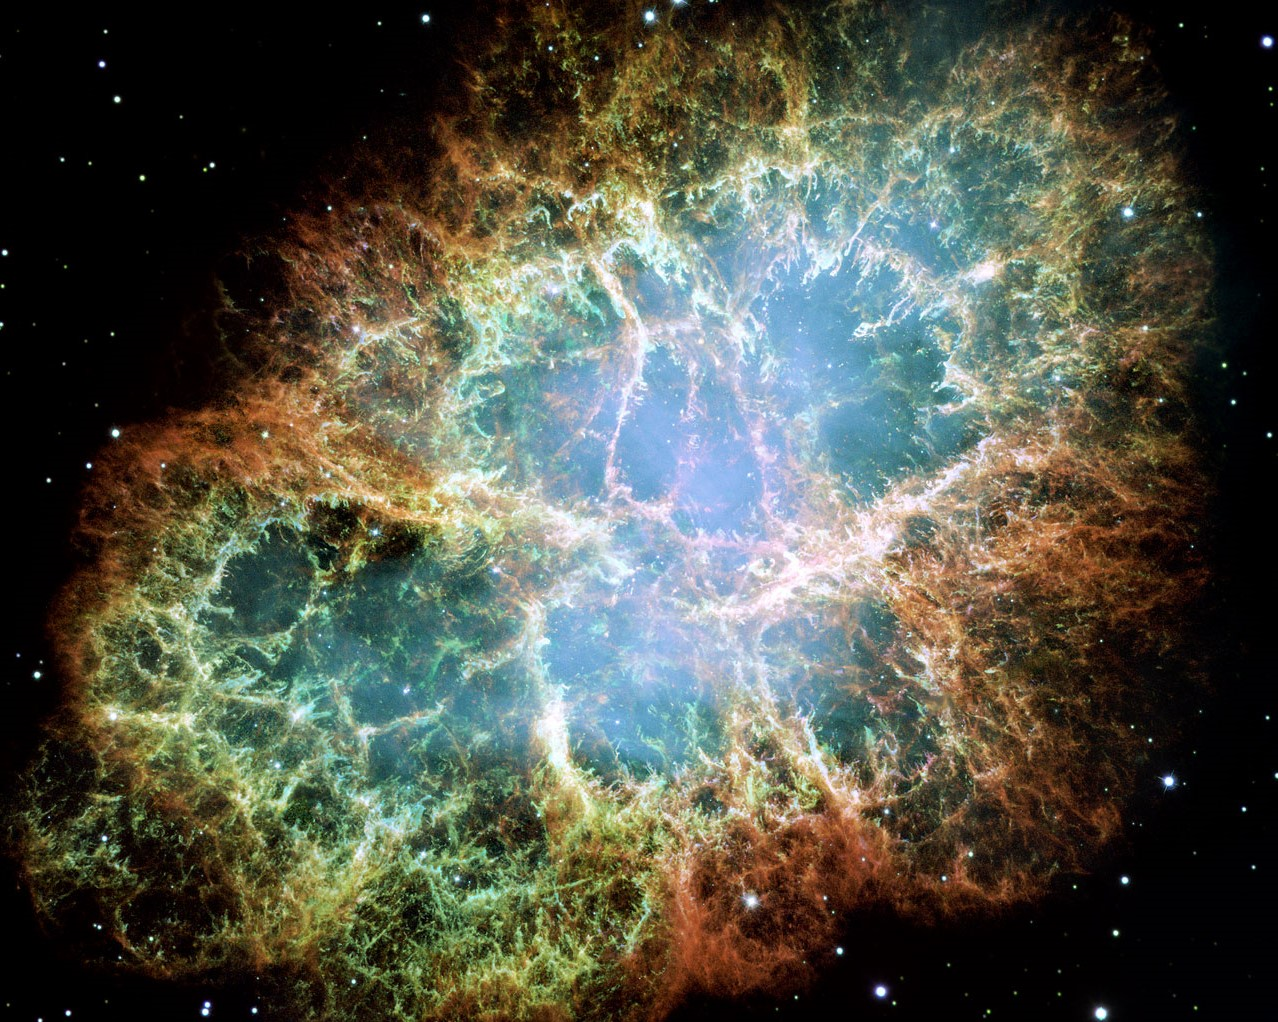
\includegraphics[width=\paperwidth, height =10cm]{../Crab.jpg}}
    \end{figure}
\end{titlepage}

%%%%%%%%%%%%%%%%%%%%%%%
\tableofcontents


%%%%%%%%%%%%%%%%%%%%%%%%%%%%%%%%%%%%% Part 1
\part{Laboratories}

%%%%%%%%%%%%%%%%%%%%%% Chapter 1.1
\chapter{Pendulum}

\section{Background}

A simple pendulum is a mass attached to a string. The time needed for one full oscillation (period, $T$) is related to the length of the pendulum $L$ and acceleration due to gravity $g$. The relationship is given by the following equation: \begin{equation}\label{eq:Pend1}
    T = 2\pi \sqrt{\frac{L}{g}}
\end{equation}
The pendulum can be used to determine the acceleration due to gravity by measuring its length and period of oscillation.

In each part of the experiment you will measure the length of the pendulum and its period (with uncertainties) in order to calculate the acceleration due to gravity and determine its uncertainty. The four values of $g$ you will find will be compared to the expected value within uncertainties. The accuracy of each part of the experiment will be determined.

\section{Experimental Procedure}

\subsection{Preliminary Measurements}

First we determine the human reaction time of the measurers. \begin{itemize}[leftmargin = 50pt]
    \item[Step 1:] Start the stopwatch and attempt to stop it exactly at $t = 5.00\;s$. Record the value of the difference between the reading and $5.00\;s$ mark in Excel. Repeat three times.
    \item[Step 2:] Calculate the average reaction time of your lab section and the standard deviation associated with the distribution. This data will help you to properly determine the uncertainty in the time of the pendulum swing.
\end{itemize}

Next we measure the length of the pendulum. First appropriately define the length of your pendulum (were do you start and stop your measurement).

\subsection{Main Data Collection}

Set up the pendulum as shown in the Figure \ref{fig:Pend1}.

\begin{figure}[H]
    \centering
    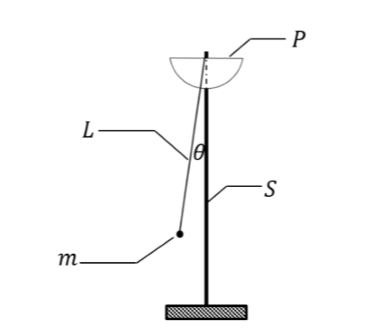
\includegraphics[scale = 0.8]{Images/Pend1.PNG}
    \caption{Experimental Setup.}
    \label{fig:Pend1}
\end{figure}

Next perform singular measurements of oscillations times:


\begin{itemize}[leftmargin = 50pt]
    \item[Step 3:] Select a string of length of approximately $1.0\;m$. Attach the selected mass to the string. Measure the length $L$ of the pendulum and record it in Excel. Estimate an uncertainty in one measurement taking into account everything discussed in preliminary measurements.
    \item[Step 4:] Measure the time $T$ for one oscillation of the pendulum. Make sure to use a small angle (less than 10 degrees) for all oscillations, as we use the small angle approximation. Record that value and determine its uncertainty $u(T)$ in Excel (use the information about the reaction time from the preliminary measurements)
    \item[Step 5:] Using the oscillation time $T$ and the length of the pendulum $L$, rearrange equation \ref{eq:Pend1} to calculate the acceleration due to gravity $g_1$. Use uncertainty propagation to calculate uncertainty $u(g_1)$.
\end{itemize}

Multiple measurements of an oscillation time:


\begin{itemize}[leftmargin = 50pt]
    \item[Step 6:] Repeat the measurement of a single oscillation ten times. Record the values in your Excel. Estimate the uncertainty of each time measurement.
    \item[Step 7:] Determine the average value of the period of the pendulum $\overline{T}$ and its uncertainty.
\end{itemize}

In this part of the lab we are deriving a Type A uncertainty for the period. Does this encapsulate all of your uncertainty about the measurement? 


\begin{itemize}[leftmargin = 50pt]
    \item[Step 8:] Using the Average period of the oscillation $\overline{T}$ and the length of the pendulum $L$ determined in the previous section, calculate the acceleration due to gravity $g_2$ and its uncertainty $u(g_2)$.
\end{itemize}

Singular measurement of time of multiple oscillations:


\begin{itemize}[leftmargin = 50pt]
    \item[Step 9:] Measure the time $t$ of ten oscillations of the pendulum and estimate the uncertainty in your time measurement. Record your results in Excel.
    \item[Step 10:] Using the time $t$ of ten oscillations, calculate the period of one oscillation $T$ with the uncertainty $u(T)$. Use the uncertainty propagation to calculate $u(T)$.
    \item[Step 11:] Using the oscillation time $T$ and the length of the pendulum $L$ from the first section, determine the acceleration due to gravity $g_3$ with uncertainty $u(g_3)$.
\end{itemize}

Measurements of multiple oscillations for various pendulum lengths:


\begin{itemize}[leftmargin = 50pt]
    \item[Step 12:] Discuss the six different values of length you are going to use and why. You can all use the same lengths or different ones. Discuss the advantages of each approach and justify your decision in the report.
    \item[Step 13:] Set up a pendulum of a given length $L$. Record the length and its uncertainty.
    \item[Step 14:] For each length, measure the time of ten full oscillations of the pendulum. Perform this experiment only once for each length. Record the values in Excel. Estimate the uncertainty of each time measurement.
\end{itemize}

When plotting our data we want it linearized in the form $y = mx+b$, so if we want period versus time we can plot $y = T$ and $\sqrt{L} = x$ so that $m = 2\pi/\sqrt{g}$.






%%%%%%%%%%%%%%%%%%%%%% Chapter 1.2
\chapter{Pendulum II}


\section{Background}

In the previous experiment the angular position of the pendulum was modeled using simple harmonic motion and it was assumed to depend on time according to the equation \begin{equation}\label{eq:Pend2}
    \theta(t) = \theta_0\cos(\omega t+\theta_i)
\end{equation}
where $\theta_0$ is the maximum angular displacement of the pendulum from its equilibrium position, $\theta_i$ is the initial displacement angle, and $\omega$ is the angular frequency of the oscillation. Equation \ref{eq:Pend2} is a solution of the ordinary differential equation \begin{equation}\label{eq:Pend3}
    \frac{d^2\theta}{dt^2} = -\frac{mgd}{I}\theta
\end{equation}
where $I$ is the moment of inertia of a pendulum about the pivot point, $m$ is the mass of the pendulum, $g$ is the acceleration due to gravity, and $d$ is the distance between the axis of rotation and the pendulum's center of mass. For the simple pendulum consisting of a string of negligible mass and a small bob of mass $m$ the moment of inertia $I = mL^2$ and $d \approx L$. Equation \ref{eq:Pend3} simplifies to \begin{equation}\label{eq:Pend4}
    \frac{d^2\theta}{dt^2} = -\frac{g}{L}\theta = -\omega^2\theta
\end{equation}
From that we can conclude that the period of the pendulum undergoing simple harmonic motion can be written as: \begin{equation}\label{eq:Pend5}
    T = \frac{2\pi}{\omega} = 2\pi\sqrt{\frac{L}{g}}
\end{equation}
All of these equations are results of the approximation $\sin\theta \approx \theta$, which is valid for $\theta$ measured in radians when $\theta < 10^{\circ} \approx \frac{\pi}{16}$.

This experiment we will consider the measurement of the period of a simple pendulum that is not constrained by the small angle approximation. We will investigate the limitations of the model, the experimental set up, and data collection procedures.


\section{Experimental Procedure}

\subsection{Preliminary Measurements}

\begin{itemize}[leftmargin = 50pt]
    \item[Step 1:] Using your experience from last week, design an experiment that will allow you to test the validity of the small angle approximation, i.e., a set up and data collection procedure that will allow measurement of the period with high precision and accuracy so it would be possible to detect whether Equation \ref{eq:Pend5} holds for larger amplitudes: \begin{enumerate}
            \item Write down a plan for a high-precision measurement of the period of the pendulum at different amplitdues andor for different pendulum sizes.
            \item Provide a clear description on the method that will be used for determining the uncertainty in the measurement.
    \end{enumerate}
    \item[Step 2:] Set up the designed experiment using the equipment provided.
    \item[Step 3:] Test your experimental setup and the method of obtaining the period of the pendulum by performing the experiment for a small angle first.
    \item[Step 4:] Check the quality of your data. Compare the value of the period to the values obtained previously. Redesign the experimental set up if issues arise.
\end{itemize}

\subsection{Main Data Collection}

First we perform a period dependence investigation:


\begin{itemize}[leftmargin = 50pt]
    \item[Step 5:] After committing to the experimental set up, collect data that shows the dependence of the period of the pendulum on the initial amplitude of the oscillation $(T(\theta_i))$. Obtain as large of a range of $\theta_i$ as you can possibly get.
    \item[Step 6:] Using Excel, plot $T(\theta_i)$ using your data and a theoretical plot $T(\theta_i)$ using Equation \ref{eq:Pend5} for your pendulum.
    \item[Step 7:] Discuss similarities and discrepancies between the experimental and theoretical curves.
\end{itemize}

Now look at your initial experiment as a scientist measuring an unfamiliar phenomenon. This will require you to focus on one or more aspects of the deviation from the small angle model. 


\begin{itemize}[leftmargin = 50pt]
    \item[Step 8:] Investigate one of the aspects of the model listed below: \begin{enumerate}
            \item The issue of $\theta_{critical}$: How precisely can you determine where small angle approximations break down? Consider the precision of the measurement, statistical distributions, and any other factors that could affect your measurement.
            \item The issue of $\theta_{max}$: As a physical system, the mass on a string will be affected by factors disregarded in the model. What are the physical limitations of the measurement? What is the maximum range of angles for which $T(\theta_i)$ can be determined?
            \item The issue of theroetical $T$. As Equation \ref{eq:Pend5} is no longer valid for large $\theta_i$, it is unlikely the relationship between $T$ and $L$ will be the same. What would that relationship look like? What other factors would the period of the pendulum depend on?
    \end{enumerate}
    \item[Step 9:] Formulate a hypothesis for any branch. Like all hypotheses, justification and logical processes that lead to the hypothesis should be included.
    \item[Step 10:] Plan your experiment. Clearly indicate all the measurements you will take.
    \item[Step 11:] Set up your experiment and collect data.
\end{itemize}


\section{Data Analysis}


\begin{itemize}[leftmargin = 50pt]
    \item[Step 12:] Plot your data to show the period dependence on the amplitude
    \item[Step 13:] Discuss similarities and discrepancies between the experimental and theoretical curves
    \item[Step 14:] Plot any additional data collected.
    \item[Step 15:] Search for existing theoretical wor kand models deriving an equation for the period of the pendulum without the small angle approximation. Properly reference sources in \Emph{Canadian Journal of Physics} style.
    \item[Step 16:] Compare the theoretiacl results and trends with those shown by your data.
\end{itemize}






%%%%%%%%%%%%%%%%%%%%%% Chapter 1.3
\chapter{AC Measurements and Sources}

\begin{figure}[H]
    \centering
    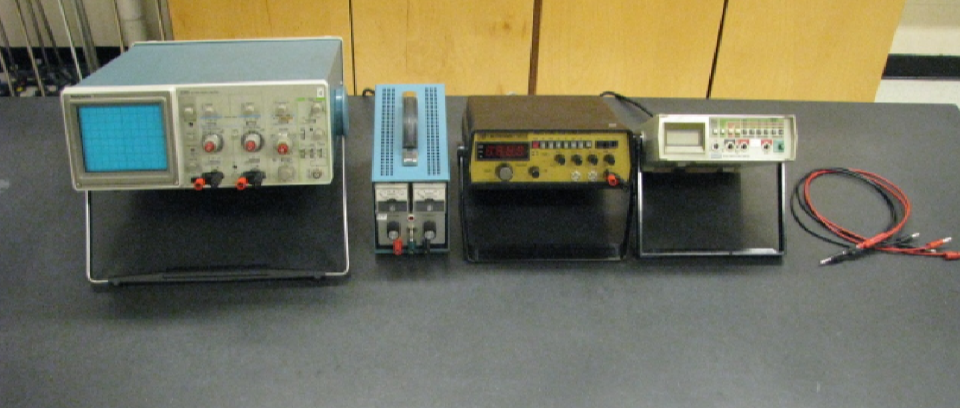
\includegraphics[scale = 0.8]{Images/ACDCSetup.PNG}
    \caption{A photo of the experimental setup.}
    \label{fig:ACDCSetup}
\end{figure}


\section{Background}

Almost all devices operate and communicate using time-varying electrical signals and therefore, the ability to measure the properties of these signals (amplitude, time variation, etcetera) is critical. The DC signals (signals that do not vary in time) are generated with a power supply while AC signals (signals that are time varying) are generated with a function generator in this lab. 

\subsection{DC Voltage Measurements}

A \Emph{multimeter} is a good choice for measuring a steady voltage, such as that across the terminals of a power supply, but an \Emph{oscilloscope} can also be used, provided that great accuracy is not required. It is instructive to measure the terminal voltage of a power supply with both a multimeter and an oscilloscope and combare results as in Figure \ref{fig:ACDC2}.

\begin{figure}[H]
    \centering
    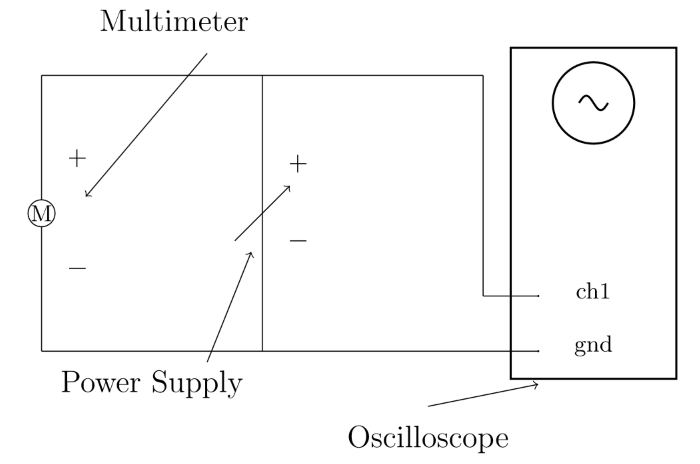
\includegraphics[scale = 0.8]{Images/ACDC1.PNG}
    \caption{Measuring DC power supply with oscilloscope and multimeter.}
    \label{fig:ACDC2}
\end{figure}

Both the reading on the multimeter and the displacement of the trace on the oscilliscope (difference between the position of the trace at \emph{ground} and when the source is connected) represent the voltage provided by the power supply. Note that the oscilloscope trace only moves when the input coupling control is set to DC. In AC coupling mode the DC component of the input signal is blocked and the trace will remain stationary. 

\begin{note}
    The oscilloscope only measures voltage, so when current is being measured it should be removed from the circuit.
\end{note}

\subsection{AC Voltage Measurement}

An oscilloscope is most useful for measuring time varying signals. Replace the power supply in the circuit with a sine function generator as seen in Figure \ref{fig:ACDC3}

\begin{figure}[H]
    \centering
    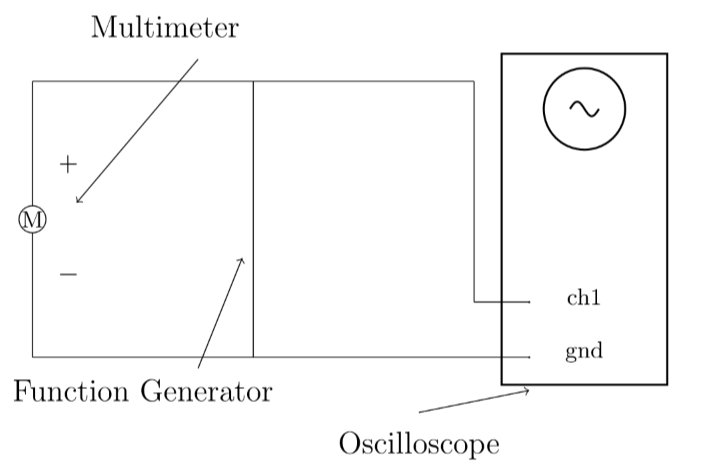
\includegraphics[scale = 0.8]{Images/ACDC2.PNG}
    \caption{Measuring AC power supply with oscilloscope and multimeter.}
    \label{fig:ACDC3}
\end{figure}

The multimeter reading can now be compared to the oscilloscope display. The trace on the display is a sine wave $V(t)$ whose equation is given by \begin{equation}\label{eq:ACDC1}
    V(t) = V_p\sin(\omega t) = V_p\sin(2\pi ft) = V_p\sin\left(\frac{2\pi}{T}t\right)
\end{equation}
where $\omega$ is the angular frequency of the wave in radians/second, $f$ is the frequency of the wave in Hertz, $T$ is the period of the wave in seconds, and $t$ is the time in seconds.

\noindent There are four ways of describing the magnitude of the AC waveform:
\begin{itemize}
    \item[a)] The \Emph{peak value} $V_p$ is the maximum voltage of the waveform. 
    \item[b)] The peak to peak value $V_{p-p}$ is the full voltage difference between maximum and minimum values of the voltage. For the sinusoidal wave given by Equation \ref{eq:ACDC1} this equals $2V_p$
    \item[c)] The average value $V_{av}$ over half a period. This value is found from the equation \begin{equation}\label{eq:ACDC2}
            V_{avg} = \frac{2}{T}\int_0^{T/2}V(t)dt = \frac{2}{T}\int_0^{T/2}V_p\sin(\omega t)dt = \frac{2V_p}{\pi}
    \end{equation}
    \item[d)] The effective or \Emph{root mean square} (RMS) value, $V_{rms}$, is defined as the equivalent DV voltage that will supply the same power, $P$, to a resistance, $R$, as the original waveform over a full period. From the definition of power:\begin{equation}\label{eq:ACDC3}
            P=\frac{1}{T}\int_0^T\frac{V^2(t)}{R}dt = \frac{1}{T}\int_0^T\frac{V_p^2}{R}\sin^2(\omega t)dt = \frac{V_p^2}{2R}
    \end{equation}
        By the above definition, the RMS voltage is that DC voltage which would supply the same power to the resistor. Therefore, \begin{equation}\label{eq:ACDC4}
            P = \frac{V_{rms}^2}{R} = \frac{V_p^2}{2R}
        \end{equation}
        and thus \begin{equation}{eq:ACDC5}
            V_{rms} = \sqrt{RP} = \sqrt{\frac{1}{T}\int_0^TV^2(t)dt} = \sqrt{\frac{1}{T}\int_0^TV_p^2\sin^2(\omega t)dt} = \frac{V_p}{\sqrt{2}}
        \end{equation}
\end{itemize}

\noindent These different \Emph{magnitudes} can be seen in the sine wave shown in Figure \ref{fig:ACDC4}.

\begin{figure}[H]
    \centering
    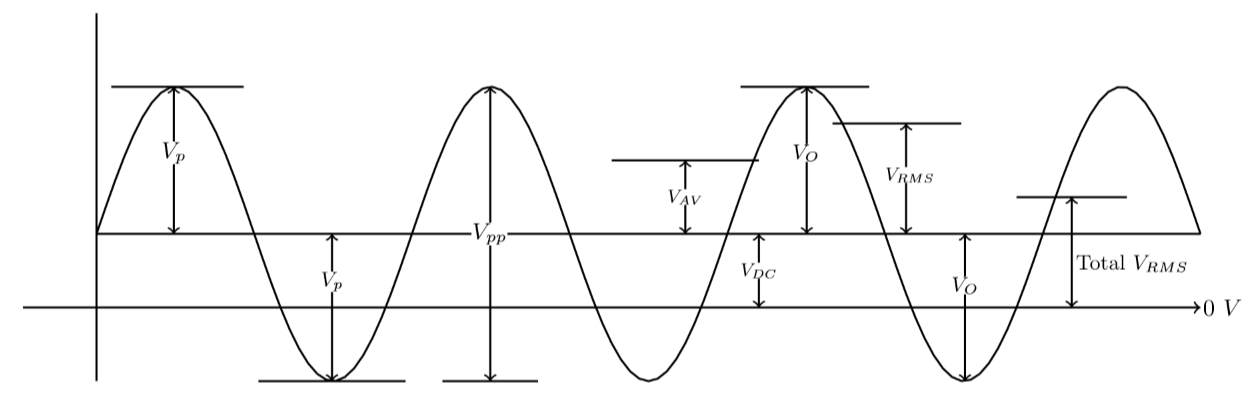
\includegraphics[scale = 0.7]{Images/ACDC3.PNG}
    \caption{The four ways of defining the amplitude of a sine wave.}
    \label{fig:ACDC4}
\end{figure}


\subsection{AC and DC Measurements}

The offset control on the function generator can be used to add a DC component to the output waveform. This can be seen in Figure \ref{fig:ACDC4} where the wave is offset vertically. THe sine wave can be observed to move up and down on the oscilloscope when the offset control is adjusted. As with the power supply, one can see that the trace will only move when the input controls are set to DC coupling. With AC coupling the DC level is removed and only the sine wave appears on the screen. Similarly, when the multimeter is set to read AC volts or amps, only the AC component is measured. When the multimeter function is DC volts or amps, only the DC level is measured.

\noindent The equation of a sinusoidal wave together with a DC level is given by \begin{equation}\label{eq:ACDC6}
    V(t) = V_p\sin(\omega t)+V_{DC}
\end{equation}
Here the frequency is the same as in Equation \ref{eq:ACDC1} but the values of $V(t)$ are different. The sinusoidal wave with extra DC component would supply more power to a resistor compared to the wave with $V_{DC} = 0 \; V$. For the case of a waveform riding on top of a DC level, the RMS amplitude is given by the formula \begin{equation}\label{eq:ACDC7}
    Total\;V_{rms_{DC}} = \sqrt{V_{rms}^2+V_{DC}^2}
\end{equation}
which for the wave described by Equation \ref{eq:ACDC6} reduces to \begin{equation}\label{eq:ACDC8}
    Total\;V_{rms_{DC}} = \sqrt{\frac{V_p^2}{2}+V_{DC}^2}
\end{equation}


\subsection{The Function Generator}

The \Emph{function generator} is an instrument that generates time varying electrical signals. The front panel controls set the shape, size, rate, and other properties of the output waveform. The BK 3011B can generate sine waves, triangle waves, and rectangular waves in a frequency range from $0.2\;Hz$ to $2.0\;MHz$.

\noindent Before connectin the function generator into a circuit, it is essential to make sure that it has been properly configured for the appropriate output signal. Standard practice is to use an oscilloscope to view the output of the function generator directly. Once the waveform is correctly displayed on the screen, the function generator is powered off and connected to the circuit. Do \Emph{not} connect an operating function generator to a circuit as it is being wired together. When the circuit wiring is completed, the function generator is powered up, along with any other power supplies and sources that the circuit needs. The function generator \Emph{cannot} withstand a short circuit across the output terminals. Always check the circuit you are driving with the function generator to make sure that the output is not being shorted out.

\begin{figure}[H]
    \centering
    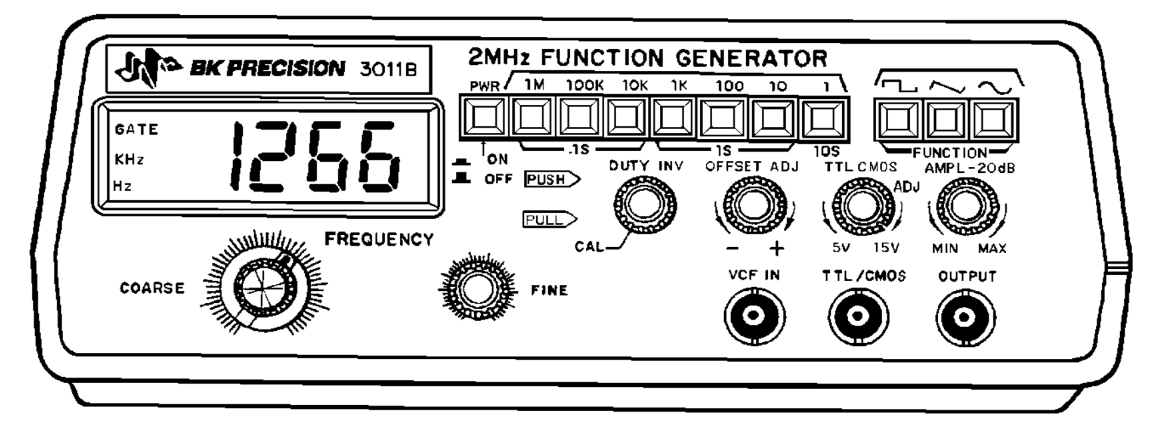
\includegraphics[scale = 0.8]{Images/ACDC5.PNG}
    \caption{BK 3011B function generator control panel.}
    \label{fig:ACDC5}
\end{figure}

Figure \ref{fig:ACDC5} shows the operating controls of the function generator. When setting up this instrument, the first task is to choose the appropriate shape (sine, square, or triangle) using the three \Emph{FUNCTION} buttons. The waveform appears at the connector labeled \Emph{OUTPUT}. The other two output jacks are not commonly used. Secondly, adjust the amplitude of the signal by adjusting the knob labeled \Emph{AMPL} to about one quarter of the way between \Emph{min} and \Emph{max}. The buttons labeled \Emph{DUTY, OFFSET, TTL}, and \Emph{AMPL} must all be pushed in. Pulling them out changes the range or adds other functions. The left knob of these four, \Emph{DUTY}, changes the symmetry of the waveform. Make sure this knob is rotated fully counterclockwise to the \Emph{CAL} position. If it is not in the proper position, some output waveforms will appear distorted.

\noindent Lastly, it remains to set how often the waveform repeats itself. The push buttons labeled $1$, $10$, $100$, $1K$, $10K$, $100K$, and $1M$ set the \Emph{range} of the repetition rate. Inside any given range the repeat rate is set by the \Emph{COARSE} and \Emph{FINE} controls. For sine waves these controls adjust the \Emph{frequency} of the wave. For triangle wave and rectangle waves, the frequency is not an accurate description adn the term \Emph{repetition rate} is used instead.

\subsection{The Oscilloscope}

An \Emph{oscilloscope} is an instrument which usually displays a graph (trace) of the voltage of a signal plotted against time. Time is plotted horizontally, in the $x$-direction and voltage is plotted vertically, in the $y$-direction. The graph changes as the voltage changes, so both the waveform and any changes in the waveform can be monitored. Both the voltage scale and the time scale can be adjusted over several orders of magnitude. Measurements of voltages and times can be made by comparing the trace wit hthe transparent scale mounted in front of the screen on which the trace appears.

\noindent The trace is formed by the motion of a bright spot which appears where a narrow electron beam hits the phosphor on the screen of a cathode ray tube (CRT). The electron beam can be deflected in the $x$ and $y$ directions by the electric field caused by amplified signals applied to deflector plates inside the tube. These amplified signals are generated inside the oscilloscope in response to controls the operator sets as well as the actual waveform to be measured.

\noindent Figure \ref{fig:ACDC6} shows the controls of a typical oscilloscope.

\begin{figure}[H]
    \centering
    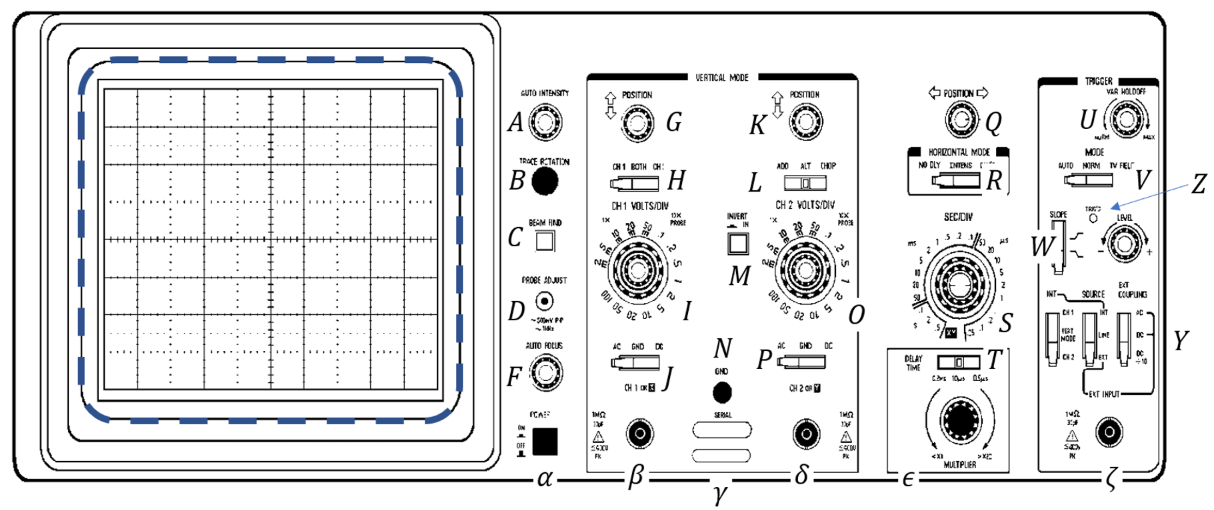
\includegraphics[scale = 0.8]{Images/ACDC6.PNG}
    \caption{Oscilloscope display panel. A - auto intensity, B - trace rotation, C - beam find, D - probe adjustments, F - auto focus, G and K - Position controls for CHANEL 1 and CHANEL 2, respectively, H and L - vertical mode switches (CH1, BOTH, CH2, ADD, ALT, CHOP), I and O - 1X and 10X probes for VOLTS/DIV range for CHANEL 1 and CHANEL 2, respectively, J and P input coupling (AC, GND (Ground), DC), M - invert, N - ground connector, Q - position control for horizontal display, R - horizontal mode switch, S - SEC/DIV switches, T - delay time range selector, U - variable holdoff control, V - more switch (auto, norm, and TV field), W - slope switch, X - level control, Y - external coupling (L), source of trigger signal (M) and internal source trigger source (R), Z - eternal input connector, $\alpha$ - power switch, $\beta$ and $\delta$ - serial and mod slots, $\gamma$ - serial and model number slots, $\epsilon$ - delay time multiplier $\zeta$.}
    \label{fig:ACDC6}
\end{figure}

We now describe the controls seen in Figure \ref{fig:ACDC6}

\begin{enumerate}
    \item Basic display controls: \begin{itemize}
            \item \Emph{Focus:} This controls the size of the spot on the screen, and thus sharpness of the trace which forms the graph. It should be adjusted to give a clear fine image.
            \item \Emph{Intensity:} This controls the brightness of the spot. If the spot is too dim the trace is too faint ot see. A trace which is too bright will eventually leave a permanent mark on the screen, and in any case tends to smear the trace and hide details. It is good practice to use the lowest intensity that will show all necessary detail in the trace without straining the eyes.
    \end{itemize}
    \item Position controls:
        
        These control the horizontal and vertical position of the trace. Usually only small changes are necessary in the horizontal position of the trace. Quite large adjustments may be needed for the vertical position. If no trace is visible on the screen, reduce the vertical gain or ground the signal using input coupling controls. Then make sure that the intensity is not too low, and set the $x$ and $Y$ position controls to the middle of their range. It may be that the time base is not triggering. Some oscilloscopes have a ``beam find" button which can be pushed to locate the trace if it off the screen.
    \item Vertical Gain:

        The vertical scale of the display is set by the vertical gain control (\Emph{SYMBOL}), usually a multi-position rotary switch. The scale is usually given in $V/cm$ or $mV/cm$. A dual trace oscilloscope has two independent sets of controls, one for each channel. If a continuous control is provided, usually a small knob in the center of the rotary switchc, make sure it is turned completely to the \Emph{CAL} position before making any measurements. Record the voltages for each channel independently as they may be set to different scales.

    \item Coupling Controls:

        The input signal can be connected (``coupled") to the amplifier for the vertical channel(s) either directly (DC coupling) or through a capacitor (AC coupling). A third possibility is to ground the input of the amplifier, which provides a quick way of finding the zero signal position of the trace. AC coupling blocks any DC component of the signal. This is useful when a varying signal is superimposed on a steady voltage, and one wants to zoom in to examine the varying part in detail. If the steady part of the signal needs to be examined then DC coupling is required.

    \item Time Base:

        The time base or sweep moves the spot horizontally to the right at a controlled speed, then returns it rapidly to the left of the screen to start again. The sweep or time-base sets the horizontal scale of the display, and is typically controlled by a multi-position rotary switch. The scale is given in $s/cm$, $ms/cm$, $\mu s/cm$, and $ns/cm$. There may be a knob at the center of the rotary switch which gives a continuous change of scale, but which clicks to a preset ``calibrated" setting when turned to the far left or right. This control must be in the ``calibrated position" before making any measurements of time intervals. It is good practice to check the appearance of the signal at a wide range of time-base settings before starting to make measurements. Some features are best seen at slow speeds while others may show up better at high speeds.

    \item Triggering:

        This controls the time at which the sweep starts. For the display to be steady the sweep should start at the same point on a repetitive signal every time the sweep begins. In this way successive traces will be in the same position:
        \begin{itemize}
            \item \Emph{Trigger Source:} The choices are usually INT (an internally generated signal being supplied to the horizontal amplifier), EXT (some external signal source), and LINE (the $60$ Hz line frequency). For most purposes INT is the correct choice. Some signal generators have a SYNC output signal which can be used to trigger the oscilloscope using EXT. The LINE trigger source is used for observing signals that are related to the AC power line. If there is a trigger mode control usually the AUTO setting is the correct one. With dual trace oscilloscopes make sure the trigger source is the appropraite channel. A channel with no signal will give poor triggering.

            \item \Emph{Trigger Level:} This sets the signal voltage value at which the sweep starts. If an AUTO mode is available, try it. If this gives a good trace use that setting. Otherwise, experiment with the LEVEL control. If the LEVEL setting is too low, the sweep will trigger at several different points in the waveform, and the successive traces will not overlap properly, giving an unstable messy display. If the level is too high, the sweep may not trigger at all, and there will be no trace, or only a dot on the left. One often has to experiment quite a lot to get a good stable trace with certain types of signal. Remember to check that the source of the trigger is the same as the signal you are actually looking at and trying to stabilize. Sometimes the trigger level has to be set carefully at one particular position to give a good stable trace, so perserverance is needed.
            \item \Emph{Trigger Slope:} One can choose whether the sweep will start with a positive or negative going part of the signal. Note that a trigger level alone is not enough to uniquely determine a position on a repetitive signal. The slope at the point must be set as well.
        \end{itemize}
\end{enumerate}


\section{Error Analysis}


The accuracy of digital meters is generally better than that of typical analog meters, but there is always some uncertainty in the calibration of any instrument. Good quality multimeters will have a statement about their accuracy on the instrument, typically on the bottom.

\subsection{Oscilloscope}

The voltage scale and time scale of the oscilloscope both have a calibration uncertainty of $3\%$ (for this lab). There is also a reading error of $4\%$ (half of the smallest division on the screen). Combining these two uncertainties in quadrature results in a measurement error for the oscilloscope of $5\%$.

\noindent This error must be applied for both time measurements and voltage measurements. The procedure to be followed to compute the uncertainty in any reading made with the oscilloscope is to add an error of $5\%$ of full scale (not the reading!). This is equivalent to one-half of a major division (or 2.5 times a minor division) for the time scale. Note that this uncertainty is much higher than that of the multimeter and constant for a given scale setting.

\noindent The digital frequency readout on the function generator has an associated uncertainty of $\pm 1$ digit.

\section{Experimental Procedure}


\begin{itemize}[leftmargin = 50pt]
    \item[Step 1:] Set up the circuit shown in Figure \ref{fig:ACDC2}. Make sure the power supply is initially set to zero volts (voltage knob fully counter-clockwise) and the current knob is turned fully clockwise.
    \item[Step 2:] Turn on both the oscilloscope and the multimeter. Set up the multimeter to measure DC voltages. Select ranges on both the scope and the multimeter for a maximum value you can comfortably observe on the screen. Set the scope to DC coupling so that DC levels can be observed.
    \item[Step 3:] For at least four different DC voltage levels, measure the output of the power supply with both the multimeter and the oscilloscope. Record your values in Excel.
    \item[Step 4:] Set up the circuit shown in Figure \ref{fig:ACDC3}. Connect the multimeter as a voltmeter. Select the sine function on the generator and a frequency of about $1.0$ kHz. To obtain a stationary trace on teh scope you will have to adjust both your time base and the frequency. A single period should almost fill the whole screen. Make sure the time base and the vertical gain are both in their calibrated positions.
    \item[Step 5:] Take a photo of the oscilloscope screen and record all relevant measurements.
    \item[Step 6:] For at least four frequencies between $100$ Hz and $1$ MHz, measure the frequency of the function generator with both the oscilloscope and the function generator panel meter. 
    \item[Step 7:] The amplitude of the sinusoidal wave can be measured with both the multimeter and the oscilloscope. Configure the multimeter for measuring AC voltage. The oscilloscope is naturally suited for measuring the peak-to-peak amplitude of a signal. From this the peak, average, and RMS amplitudes can be derived. The point of this step is to deduce which kind of amplitude the multimeter reports. For at least four different amplitudes, measure the amplitude of the sine wave using both the oscilloscope and multimeter. Each of the four sine waves should have a different frequency as well. For best results keep the frequency between $100$ Hz and $20$ kHz.
    \item[Step 8:] For four different amplitudes of a $1.0$ kHz square wave ,measure the peak and RMS voltage of the square wave, using the oscilloscope and multimeter.
\end{itemize}

Note that the DC offset control on the function generator adds a DC level to the output waveform. This suggests that readings can be compared between the multimeter and the oscilloscope for the total RMS voltage of a signal with both DC and AC components.


\begin{itemize}[leftmargin = 50pt]
    \item[Step 9:] For four different amplitudes and DC offsets of $5.0$ kHz sine wave, measure the total RMS voltage using both the multimeter and the oscilloscope. IT will be necessary to make two measurements with each instrument, one for the DC component and one for the AC component.
    \item[Step 10:] Oscilloscopes can respond to much higher frequencies than multimeters can. Measure the voltage of a sinusoidal wave with a multimeter and then increase the frequency until the multimeter has difficulty reporting a voltage.
\end{itemize}




%%%%%%%%%%%%%%%%%%%%%% Chapter 1.4
\chapter{Traveling Waves}

\begin{figure}[H]
    \centering
    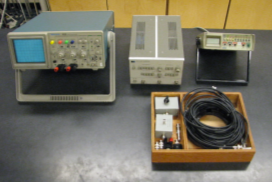
\includegraphics[scale = 1.4]{Images/TW1.PNG}
    \caption{A photograph of the experimental setup.}
    \label{fig:TW1}
\end{figure}

\section{Background}

Imagine a rope fixed to a wall and under tension at the free end. When this free end is flipped upwards once a wave travels down the rope until it reaches the wall. Here, the wave exerts a force on the wall and the wall exerts an equal and opposite force on the rope. The result is a wave opposite to the original wave traveling back on the rope in the reverse direction. The incident wave has been reflected by the wall. As a second example, suppose now that one end of the rope is free to move up and down because it has been connected to a ring that is free to slide on a frictionless rod perpendicular to the rope. Now, when the free end is flipped up once, a wave travels down the rope as before. When this wave reaches the ring the force of the wave raises the ring which then falls back down to generate a wave travelling back down the rope. Unlike the solid wall, this wave is identical to the original wave, instead of opposite.


\noindent These two examples demonstrate that a wave on a rope is reflected by both a \Emph{fixed rope termination} as well as a \Emph{free rope termination}. The fixed and free rope ends are the extreme cases. In an intermediate case, where the rope termination is partly free (or partly fixed), the incident wave will be reflected back with varying intensities and can be opposite or identical, depending on whether the termination is closer to a free end or a fixed end. This logically implies there must be one termination exactly in between which produces no reflection. This \Emph{proper termination} occurs when the rope end has a resistance to the wave that is exactly the same as the resistance of the rope itself. From the point of view of the rope, the wave continues onward without interruption because the wave only sees more identical rope ahead. From the point of view of an external observer, the proper termination has absorbed the wave and produced no reflection. This single value of resistance that absorbs waves instead of reflecting them is called the \Emph{characteristic impedance}, $Z_0$. If the rope were thinner or more compliant the characteristic impedance would change.


\noindent A second wave property of the rope is the velocity at which the wave propagates along the rope. Giving a harder flip will increase the amplitude of the wave but it will not travel down the rope any faster. This \Emph{velocity of propagation}, $V_p$, is dependent on the thickness and compliance of the rope. One can image reversing the rope so the formerly terminated end is now the end to be flipped. The waves will propagate and reflect on the rope the same as before. For the rope then, the characteristic impedance and velocity of propagation are identical for the the forward traveling waves and the reverse traveling reflected waves.

\noindent What happens if the rope is flipped twice so that the reflected wave from the first flip must cross the incoming wave of the second flip? The result is determined by a third property of the rope called the \Emph{principle of superposition}. This principle states that when two waves overlap, the resulting vertical displacement of the rope (the height or amplitude), is the sum of the individual displacements of each wave. The waves themselves do not interfere with each other. After the waves have crossed, each carries on as before without any change in speed or amplitude.

\noindent If the rope were ideal, or \Emph{lossless}, then the traveling waves would never lose any energy. In practice, a wave traveling on a rope loses a constant fraction of its amplitude per meter of travel along the rope. This \Emph{attenuation}, or \Emph{loss factor}, of the rope is a fourth characteristic property of the rope. Due to attenuation, a wave traveling on a very long rope will slowly decay away. In this experiment you will be observing and verifying each of these four properties.

\noindent The waves on a rope are an example of a mechanical traveling wave. Traveling wave phenomena occur in any situation where the travel time of a wave along the medium is significantly larger than the size of the wave. Examples of this are everywhere. Bats use acoustic traveling waves in air to locate their prey and avoid obstacles. Dolphins and submarines do the same with acoustic waves in water. The wake from a boat generates surface traveling waves on top of the water that take some time to reach the shore. Striking a hammer on a steel beam generates traveling waves in a solid medium. A sudden application and removal of heat generates a heat wave that travels by conduction. The sudden diffusion that occurs when one material is added to another is also a traveling wave. Lastly, electrical signals in wires and electromagnetic waves in space furnish many examples of traveling waves.

\noindent The size and speed of a traveling wave system can vary greatly. The yearly thermal cycle on a concrete dam generates waves with widths in the tens of meters. On the other hand, in a high frequency radar set the waves travel millimeters in a few nanoseconds. This experiment will examine electrical pulses in cables several meters long. The waves will travel the length of the cable in several tens of nanoseconds. This system is used for traveling wave experiments because it closely approximates an ideal traveling wave system. Furthermore, it is easy and fast to make direct measurements on the traveling waves and the cables are small and easily handled. This experiment would not be so easy to perform with yearly thermal waves in a concrete dam.

\noindent Let $x$ be the position of the wave and $t$ the time. Then all lossless linear traveling wave systems obey the \Emph{telegrapher's equations} \begin{equation}\label{eq:TW1}
    \frac{\partial v}{\partial x} = -\frac{Z_0}{V_p}\cdot\frac{\partial i}{\partial t}
\end{equation}
and \begin{equation}\label{eq:TW2}
    \frac{\partial i}{\partial x} = -\frac{1}{V_pZ_0}\cdot\frac{\partial v}{\partial t}
\end{equation}

\noindent Since this experiment deals with electrical pulses on a cable, the variable $v$ represents the voltage and the variable $i$ represents the current. For any other traveling wave system they would represent some other relevant physical quantities. The partial derivatives are required because the wave depends on both the position and the time. Hence the voltage, $v$, is really a function $v(x, t)$, and the current, $i$, is really a function $i(x, t)$. The solutions to the telegraphers equations are \begin{equation}\label{eq:TW3}
    v(x,t) = f(x-V_pt) + g(x+V_pt)
\end{equation}
and \begin{equation}\label{eq:TW4}
    i(x,t) = \frac{1}{Z_0}\left[f(x-V_pt) - g(x+V_pt)\right]
\end{equation}
The solution functions $f$ and $g$ are arbitrary. This means it does not matter what shape the traveling wave may have, the general behaviour remains unchanged. Both the $f$ and $g$ functions each satisfy the telegrapher’s equations alone. The reason for this is that $f$ and $g$ are arbitrary, so either $f$ or $g$ could be identically zero. This allows us to examine $f$ and $g$ independently. For $f$, as long as $x$ is increased with velocity, $V_p$, the value of $f(x, t)$ remains unchanged. So $f$ is a wave traveling in the positive $x$ direction. Similarly, $g$ is a wave traveling in the negative $x$ direction. Set $g$ to zero so the forward wave can be examined. Dividing Equation \ref{eq:TW3} by Equation \ref{eq:TW4} gives  \begin{equation}\label{eq:TW5} 
    \frac{v(x,t)}{i(x,t)} = Z_0
\end{equation}
which is a travelling wave version of Ohm's law. For the reverse wave $g$, the result is \begin{equation}\label{eq:TW6}
    \frac{v(x,t)}{i(x,t)} = -Z_0
\end{equation}

\noindent It is now possible to describe reflections quantitatively. Imagine a wave traveling on a cable that is terminated in a load $Z_T$ and has a characteristic impedance $Z_0$. Let $v^+$ be the voltage traveling toward the load and $v^-$ be the voltage reflected from the load. The voltage at the load (terminated end) must be \begin{equation}\label{eq:TW7}
    v_T = v^+ + v^-
\end{equation}
and using Equations \ref{eq:TW5} and \ref{eq:TW6}, the current must be \begin{equation}\label{eq:TW8}
    i_T = i^+ + i^- = \frac{1}{Z_0}(v^+-v^-)
\end{equation}
The voltages and currents at the terminated end are determined by the load $Z_T$, which means \begin{equation}\label{eq:TW9}
    \frac{v_T}{i_T} = Z_T = \frac{v^++v^-}{v^+/Z_0 - v^-/Z_0} = Z_0 \frac{v^+ + v^-}{v^+-v^-}
\end{equation}


\noindent Define the \Emph{reflection coefficient} to be the ratio of the reflected voltage
to the incident voltage \begin{equation}\label{eq:TW10}
    \Gamma_r = \frac{v^-}{v^+}
\end{equation}
Using Equation \ref{eq:TW9} this can be rewritten as \begin{equation}\label{eq:TW11}
    \Gamma_r = \frac{Z_T-Z_0}{Z_T+Z_0}
\end{equation}
Equation \ref{eq:TW11} is our desired result.  It predicts what the reflection voltage should be for any type of termination. If the load resistance is equal to the characteristic impedance the reflection coefficient is zero. When the termination is $Z_T = 0$ (a shorted end), the reflection coefficient is $-1$. When the termination is infinite (an open end), the reflection coefficient is $+1$. This corresponds exactly to what was discussed in the rope example.

\section{Experimental Procedure}

\begin{itemize}[leftmargin = 50pt]
    \item[Step 1:] Connect the output of the pulse generator to the input of the oscilloscope through the feedthrough termination supplied on the oscilloscope. This termination makes the input of the oscilloscope have the same characteristic impedance as the output of the pulse generator so that reflections are eliminated. Set up the pulse generator for maximum amplitude and minimum pulse width. Adjust the pulse period so that the pulses (waves) are spaced 5 microseconds apart. The remaining pushbuttons on the pulse generator must be in the out position, except for \Emph{POS} and \Emph{INT LOAD} which must be pushed in. The pulse generator is now set up to generate waves that are narrow enough and spaced far enough apart that reflections can easily be observed.
    \item[Step 2:] Determine the maximum and minimum values of the pulse. Also, measure the time it takes for the signal to rise from minimum to maximum (the rise time), and from maximum to minimum (the fall time). Measure the width of the pulse at the half height point. Make two sketches or take two snapshots of this wave. One diagram should illustrate a single pulse in detail. The other diagram should illustrate what a train of pulses looks like. Include relevant measurements/annotations on the diagrams.
    \item[Step 3:] Connect the circuit shown in Figure \ref{fig:TW2}. Observe the reflected pulse and determine the time between the initial pulse and the reflected pulse. Also, measure the amplitude of the initial and reflected pulses. From these you will be able to determine the velocity of propagation and the attenuation of the wave medium (the RG58 cable). Draw a diagram. Connect a short circuit termination to the end of the cable. Draw a diagram with relevant measurements for this case. Repeat this step for the RG59 and twinaxial cables.
        \begin{figure}[H]
    \centering
    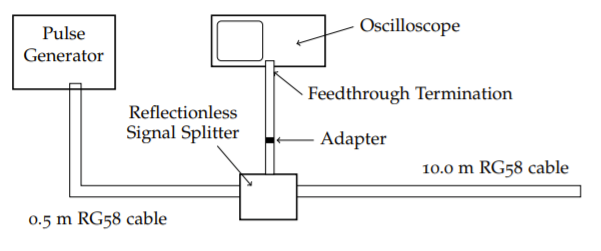
\includegraphics[scale = 0.8]{Images/TW2.PNG}
    \caption{A diagram of the experimental set up.}
    \label{fig:TW2}
\end{figure}
    \item[Step 4:] Remove the short circuit termination and connect the variable resistor termination. Adjust the resistor until there is no reflection. Remove the variable termination from the circuit and use the Fluke meter to measure its resistance. This is the value for the characteristic impedance of RG58 cable. Now vary the resistance over its entire range. At each point measure the resistance of the termination and the corresponding amplitude of the initial and reflected waves. Take enough data so that you will be able to verify or refute Equation \ref{eq:TW11}.
    \item[Step 5:] Remove the variable resistance and leave the cable end open. Increase the pulse width until the outgoing pulse overlaps the reflected pulse. Draw a diagram and take amplitude measurements that will allow you to verify or refute the principle of superposition. Decrease the pulse width back to minimum.
    \item[Step 6:] Connect the $7.0\; m$ RG59 cable to the end of the RG58 cable. Terminate the open end with a short. Sketch what you observe. Describe what each reflected wave represents. Apply the variable resistive termination to the end of the RG59 cable to measure its characteristic impedance. Repeat with the $7.0 \;m$ twinaxial cable.
    \item[Step 7:] Set up the circuit shown in Figure \ref{fig:TW3}. Connect one end of the $10.0 \;m$ RG58 cable to the t-splitter (connected to channel 1) and the other end to channel 2 of the oscilloscope via the feedthrough termination. Set the oscilloscope display to show both channels 1 and 2 and record the voltage differences between the direct output of the pulse generator and the attenuated signal from the cable. Next, measure the time separation between each pulse to determine the phase velocity of the cable. Repeat with the RG59 and twinaxial cables.
        \begin{figure}[H]
    \centering
    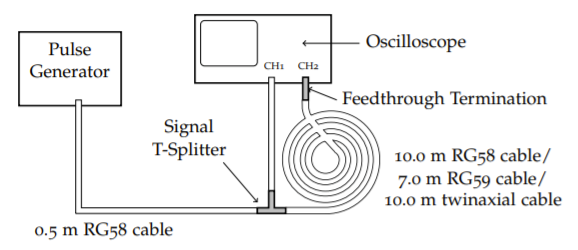
\includegraphics[scale = 0.8]{Images/TW3.PNG}
    \caption{A diagram of the experimental set up for the determination of signal attenuation in RG58, RG59, and twinaxial cables.}
    \label{fig:TW3}
\end{figure}
\end{itemize}

\section{Error Analysis}

The uncertainty in measuring the voltage and the time of the wave is the instrument error of the oscilloscope. Assume that the scale on the oscilloscope screen is a ruler. Then the error is one half of the smallest division. Each division in the horizontal direction will have a size determined by the horizontal oscilloscope setting. Similarly, a vertical division is determined by the vertical oscilloscope setting. Take the length of each cable to be exact. For the multimeter, the error is the instrument error as written on the underside of the meter.



%%%%%%%%%%%%%%%%%%%%%% Chapter 1.5
\chapter{X-Ray Diffraction}

\begin{figure}[H]
    \centering
    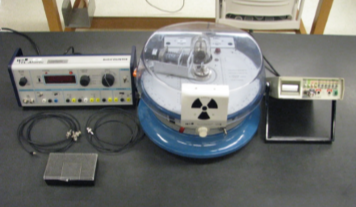
\includegraphics[scale = 1.4]{Images/XR1.PNG}
    \caption{A photograph of the experimental setup.}
    \label{fig:XR1}
\end{figure}

\section{Background}

In the late 19th century physicists and inventors began to work with a new device called a \Emph{cathode ray tube}. A cathode ray tube is a glass bulb with the air removed, a hot metal filament at one side, a metallic plate at the other end, and a high voltage between the plate and the filament. This device simultaneously started the eras of modern quantum physics and modern electronics. Among its many other properties, it was noticed that operating such a cathode ray tube at high voltages had a side effect. The cathode ray tube caused various objects outside of the tube to glow. Although other observers had noticed this effect, it was the german physicist Wilhelm Röntgen (1845-1923) who thought it might be important and undertook a systematic study of the phenomenon.

\noindent Röntgen noticed that the glow persisted even when the cathode ray tube was covered up. He called the unknown emissions originating from the cathode ray tube \Emph{x-rays}. A name which remains to this day, although they are also known as Röntgen rays in his honor. Moreover, placing a hand between the glow and the tube cast an eerie shadow that illuminated the bones inside his hand in a different light than the surrounding tissue. Röntgen found that this shadow could be photographed. Figure \ref{fig:XR2} shows one of Röntgen’s pictures, one of the earliest x-ray photographs ever taken, dating from 1895. 

\begin{figure}[H]
    \centering
    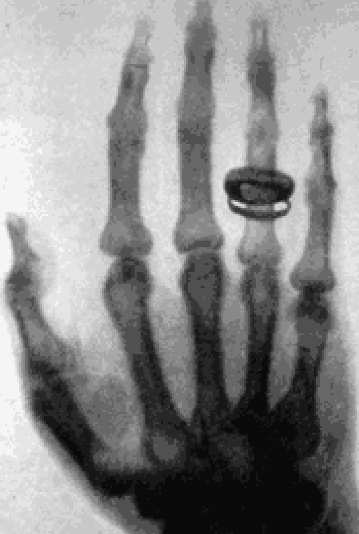
\includegraphics[scale = 0.8]{Images/XR2.PNG}
    \caption{An x-ray image of a hand}
    \label{fig:XR2}
\end{figure}

\noindent He also found that the x-rays originated in the cathode ray tube at the location where the internal cathode rays struck the metallic plate at the end of the tube. He then established that their degree of penetration through an element depended upon its atomic number. Elements of high atomic number were able to block the x-rays better. Knowing this, he was then able to use slits cut in lead to show that x-rays travel in straight lines and that they are unaffected by electric and magnetic fields. This suggested that the x-rays were a form of electromagnetic radiation similar to light. For his work on x-rays, Röntgen was given the 1901 Nobel prize in physics, the first ever awarded.

\noindent If x-rays were similar to light, it seemed reasonable to check whether they exhibit other optical properties of light such as \Emph{diffraction}. Diffraction is a wave property of light that makes the edges cast by shadows indistinct instead of sharp and can be used to separate light of different wavelengths. Subsequent investigators had difficulty observing any diffraction and began to suspect that if x-rays were electromagnetic waves like light, they must be of a greatly different wavelength. The German physicist Max von Laue (1879-1960) realized that the spacing of atoms in crystals might be suitable for observing the diffraction of x-rays. His insight was successful and he and his students were the first people to observe \Emph{x-ray diffraction} through a crystal. For this work von Laue was awarded the 1914 Nobel prize in physics.

\noindent Several more Nobel prizes were earned by physicists studying xrays. The British son and father team of Sir William L. Bragg (1890-1971) and Sir William H. Bragg (1862-1942) extended von Laue’s work. They predicted how x-rays reflect off crystals (a rule now called \Emph{Bragg's law} of x-ray diffraction) and used this to design and construct instruments that can examine x-rays by their wavelength. Such instruments are now called \Emph{Bragg x-ray spectrometers}. For their work the Bragg’s received the 1915 Nobel prize in physics. Further work by the British physicist Charles Barkla (1877-1944) established how x-rays are scattered, polarized, and absorbed. He also discovered that when one of its electrons transitions to higher energy level each element emits its own characteristic wavelengths of x-rays which he named \Emph{K-shell x-rays}. For this work Barkla received the 1917 Nobel prize in physics. More results on x-ray atomic spectra and still greater refinement of x-ray spectrometers earned the Swedish physicist Karl Siegbahn (1886-1978) a Nobel prize in 1924.


\noindent It is now accepted that x-rays are a relatively high energy form of electromagnetic radiation with a much shorter wavelength than light. Ultimately, x-rays became a standard diagnostic tool universally used by astronomers, biologists, chemists, dentists, doctors, engineers, geologists, and physicists. The penetrating nature of x-rays makes it possible to image the interior of living organisms, observe cracks hidden in structures and mechanisms, discern the behaviour of energetic astronomical objects, study the arrangement of atoms in crystals, powders, and alloys, determine the composition of surfaces, and probe the internal energy levels of atomic isotopes.

\noindent A point most of these x-ray applications have in common is that they require an x-ray generator, a source of x-rays. Aside from refinements, the \Emph{x-ray tubes} used in modern x-ray generators (and the x-ray tube used in this experiment) have the same structure as the original xray tubes Röntgen used. Figure \ref{fig:XR3} shows the structure of an x-ray tube. A hot \Emph{cathode} inside an evacuated glass tube emits electrons. These electrons are accelerated to the other end of the tube by a high voltage and strike the metal target, called the \Emph{anode}. This \Emph{electron beam} has enough energy to directly interact with the atoms in the target anode. Most of this energy (about $95\%$) is lost in the target as heat. The remainder of the energy is converted into x-rays. The target is \Emph{bevelled} to give some directionality to the emitted x-rays. Further control of the x-ray beam path is achieved by a lead glass envelope that blocks x-rays in all directions, except for the \Emph{aperture} through which the x-rays are permitted to pass.

\begin{figure}[H]
    \centering
    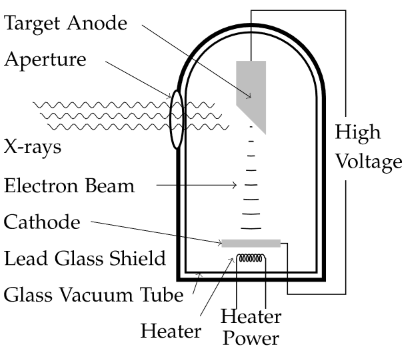
\includegraphics[scale = 0.8]{Images/XR3.PNG}
    \caption{Schematic representation of an x-ray tube.}
    \label{fig:XR3}
\end{figure}

\noindent The x-rays generated by a typical x-ray tube cover a broad range of wavelengths. The proportion of x-rays at any given wavelength is governed by the physical interaction processes between the electrons in the electron beam and the atoms inside the target. A typical spectrum of x-rays emitted by an x-ray tube is shown in Figure \ref{fig:XR4}. It can be seen that the spectrum exhibits two main features. There is a broad curve at all wavelengths to the right of a certain value. Superimposed on this is a set of sharp peaks. It has been found that the shape of the smooth part is determined by the magnitude of the high voltage and the aperture material. The positions and relative sizes of the sharp peaks are determined by the type of atoms the target anode is composed of.

\begin{figure}[H]
    \centering
    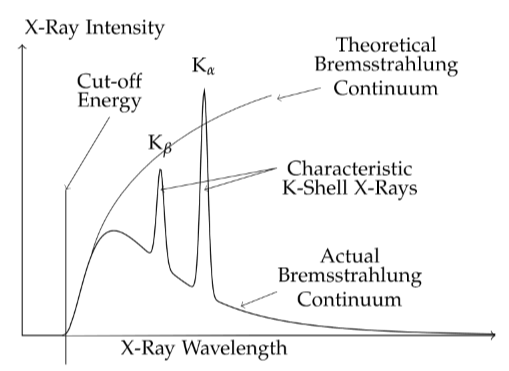
\includegraphics[scale = 0.8]{Images/XR4.PNG}
    \caption{An example of an x-ray spectrum.}
    \label{fig:XR4}
\end{figure}

\noindent The smooth broad curve is known as the \Emph{bremsstrahlung continuum}. This bremsstrahlung radiation, or \Emph{braking radiation}, arises due to the acceleration the electrons undergo when they strike the target anode and interact with the electric fields of the atoms inside. Electromagnetic theory predicts that accelerated charges will radiate electromagnetic waves. The large number of electrons in the electron beam are all accelerating in different ways since they interact with different atoms of the target at a variety of distances. So the radiated electromagnetic energy happens at many wavelengths and this yields the continuum.

\noindent According to the quantum picture, this radiation will be in the form of photons with energy $E = hf$ corresponding to the change in the electron kinetic energy $\Delta K$, so that \begin{equation}\label{eq:XR1}
    E = hf = \Delta K
\end{equation}
where $f$ is the frequency of the photon, and $h = 6.62606876\times 10^{-34}\;Js$ is \Emph{Planck's constant}.

\noindent The most energetic possible photon occurs when the electron loses all of its kinetic energy in a single interaction. For an x-ray tube with accelerating voltage, $V$, the maximum photon energy, $E_{max}$, and corresponding minimum wavelength $\lambda_{min}$ is \begin{equation}\label{eq:XR2}
    E_{max} = hf_{max} = \frac{hc}{\lambda_{min}} = eV
\end{equation}
where $e = 1.60217646\times 10^{-19}\;C$ is the charge of an electron and $c = 299792458\;m/s$ is the speed of light. This highest energy is known as the \Emph{cut-off energy} of the x-ray tube. An x-ray tube cannot generate x-rays with higher energy than the cut-off energy. At the low end of the spectrum, it seems reasonable to expect that low energy x-rays would be produced in much greater quantities than high energy x-rays near the cut-off. Theoretically, this is indeed correct as can be seen by the theoretical curve shown in Figure \ref{fig:XR4}. However, in practice, it turns out that the low energy x-rays are not detected in great numbers. The reason for this is that low energy x-rays are easily absorbed. The lowest energy x-rays do not even make it out of the target material. Still more are blocked by the glass walls of the x-ray tube, the air, and the entrance walls of the x-ray detector. This results in the characteristic shape of the bremsstrahlung spectrum seen in Figure \ref{fig:XR4}, where numbers of x-rays are small at low energies, increase to some maximum, and then decrease back down to zero at the cut-off. 

\noindent The other feature of the x-ray tube spectrum is seen to be the sharp peaks that rise above the bremsstrahlung continuum. These peaks are also due to interactions between the electrons in the electron beam and the atoms in the target. The energy level model of the atom implies that the electrons surrounding the nucleus of an atom have different energy levels called \Emph{shells}. Each electron shell has a designated \Emph{principal quantum number}, $n$. As seen in Figure \ref{fig:XR5}, the innermost shell has quantum number $n=1$ and is commonly called the \Emph{K-shell}. The next shell outward has quantum number $n=2$ and so on. Any transition of an electron from one level to a lower level must be accompanied by the emission of a photon of energy equal to the energy difference between the two levels.

\begin{figure}[H]
    \centering
    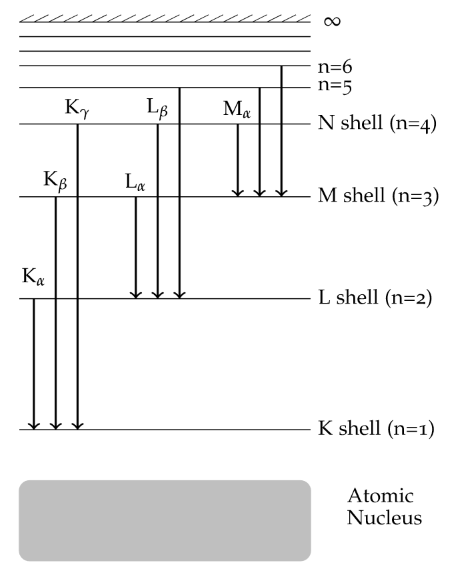
\includegraphics[scale = 0.8]{Images/XR5.PNG}
    \caption{Diagram representing electronic energy levels in an atom.}
    \label{fig:XR5}
\end{figure}

\noindent Electrons in the electron beam of the x-ray tube which are sufficiently energetic can penetrate into the atoms and knock an electron out of an inner shell. In turn, an electron from a higher energy level falls down to fill the hole in the inner shell and thereby releases a photon of the corresponding energy difference. So, for example, when an inner electron from the K-shell is removed from the atom, a common transition is for an electron in the next higher shell ($n = 2$) to move into the inner shell and emit a photon. As seen in Figure \ref{fig:XR5}, this photon is named $K_{\alpha}$. It turns out that for many materials, the $K_{\alpha}$ photon (and many others) happens to have sufficient energy to be an x-ray photon. Each element has a characteristic set of x-ray peaks corresponding to transitions of electrons between inner energy levels. The height of each peak is related to the probability that the particular electron transition corresponding to that energy difference can happen. These \Emph{characteristic x-rays} serve as an identifying marker that can be used to identify the target material and explore its inner atomic energy levels.

\noindent It is therefore of strong interest to find a method to determine the wavelengths of the features seen in the x-ray spectrum because the actual wavelengths could be used to measure the energy levels of electronic orbitals inside the atom. What is needed is a device that can separate x-rays by their wavelength. For visible light, the device commonly used for this purpose is called a \Emph{diffraction grating}. It consists of a large number of equally spaced parallel lines inscribed onto glass. The spacing of the lines is critical to the operation of the grating. For useable results, the separation between the lines should be roughly the same size or smaller than the wavelength of the light to be diffracted. So for visible light with a wavelength around $500 \;nm$, the spacing of the lines needs to be at least 200 lines per millimeter. Unfortunately, it turns out that the wavelength of x-rays is about 1000 times smaller than the wavelength of visible light. It is quite difficult to machine lines fine enough to serve as a diffraction grating for x-rays. However, the spacing between atoms in a regular solid such as a crystal serves very well as a natural diffraction grating for x-rays.


\begin{figure}[H]
\centering
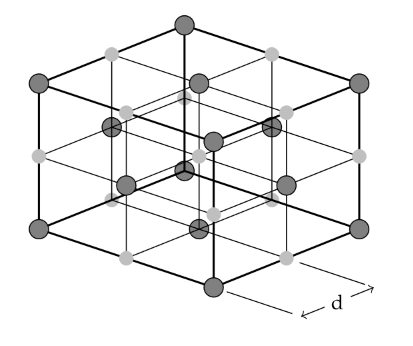
\includegraphics[scale = 0.8]{Images/XR6.PNG}
\caption{Crystalline structure of Lithium Flouride.}
\label{fig:XR6}
\end{figure}


\noindent This natural correspondence between the x-ray wavelength and the spacing of atoms enables crystals to be used as diffraction gratings for x-rays. The study of crystals and x-rays constitutes the scientific field of \Emph{x-ray crystallography}. There is a large abundance of different types of crystals, each with their own structure and properties. This experiment restricts its attention to the simplest type of crystal, an ionic solid with a cubic structure as seen in Figure \ref{fig:XR6}. The most common example of this type of solid is ordinary table salt, NaCl. Unfortunately, salt crystals have a tendency to absorb water and break down. For this reason, the cubic ionic crystal used in this experiment instead is Lithium Fluoride, LiF. As seen in Figure \ref{fig:XR7}, each atom of lithium is surrounded by six fluorine atoms and conversely, each fluorine atom is surrounded by six lithium atoms. All of the atoms are the same distance from each other and this gives rise to the cubic crystal structure

\begin{figure}[H]
    \centering
    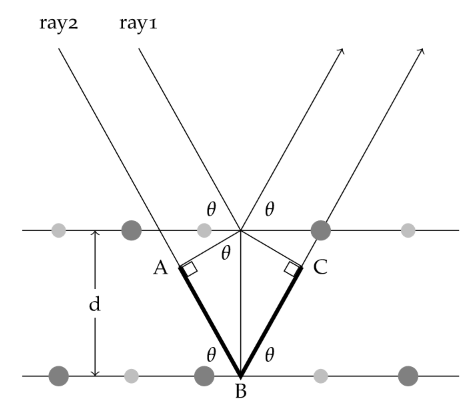
\includegraphics[scale = 0.8]{Images/XR7.PNG}
    \caption{A geometrical perspective on x-ray interaction with a LiF substrate.}
    \label{fig:XR7}
\end{figure}

\noindent It seems reasonable to expect that the spacing between the atoms in the LiF crystal influences how the x-rays diffract through the crystal in the same way that the spacing between ruled lines determines how visible light diffracts through an optical diffraction grating. The cubic structure of LiF makes it possible to calculate the distance between the atoms. Let the \Emph{atomic mass} of lithium be denoted by $A_{Li}$ and the atomic mass of fluorine be denoted by $A_F$. Then the molar mass, $A_{LiF}$, of lithium fluoride is given by\begin{equation}\label{eq:XR3}
    A_{LiF} = A_{Li} + A_F
\end{equation}
The number of molecules in $A_{LiF}$ (one mole) grams of LiF is $N_A$, where $N_A = 6.02214199\times 10^{23}$ is \Emph{Avogadro's number}. If the density of LiF is $\rho$ grams per cubic centimeter, then the volume, $V$, of $N_A$ molecules of $LiF$ must be \begin{equation}\label{eq:XR4}
    V = \frac{A_{LiF}}{\rho}
\end{equation}
cubic centimeters. Since LiF is \Emph{diatomic}, the \Emph{atomic spacing}, $d$, in centimeters between the atoms in LiF is \begin{equation}\label{eq:XR5}
    d = \sqrt[3]{\frac{A_{LiF}}{2N_A\rho}}
\end{equation}

\noindent To calculate how the diffraction of x-rays happens inside an LiF crystal, assume that the LiF has a cubic structure and that the x-rays actually are electromagnetic waves. The separation, $d$, between two neighboring atomic planes is then given by Equation \ref{eq:XR5}. Imagine two x-rays, ray1 and ray2, with wavelength, $\lambda$, reflecting off of two planesof atoms inside the crystal with angle of incidence $\theta$ as seen in Figure \ref{fig:XR7}. For electromagnetic waves, the angle of reflection equals the angle of incidence, so the reflected ray also leaves the crystal at the same angle $\theta$. If ray1 and ray2 are parallel, then the extra distance travelled by ray2 is the length of the two line segments $AB$ and $BC$. For constructive interference to occur, the distance $AB+BC$ must be an integer multiple of the wavelength. So when x-rays reflect off of the surface of a LiF crystal, each wavelength reflects at a particular angle and all the other wavelengths cancel out. The length of $AB$ is $d\cdot \sin(\theta)$, so the condition for constructive interference is \begin{equation}\label{eq:XR6}
    n\lambda = 2d\sin(\theta)\;\;\;\;n=1,2,3,...
\end{equation}
This formula is known as \Emph{Braggs law} and it describes how x-rays diffract when reflected by a cubic crystal. This diffraction interaction is called \Emph{Bragg x-ray diffraction} and it implies that a LiF crystal can be used to measure the wavelength of x-rays simply by tilting it at different angles to the x-ray beam.


\noindent The instrument that measures an x-ray spectrum by taking advantage of Bragg’s law is called a \Emph{Bragg x-ray spectrometer}. The construction of a typical Bragg x-ray spectrometer is shown in Figure \ref{fig:XR8}.

\begin{figure}[H]
    \centering
    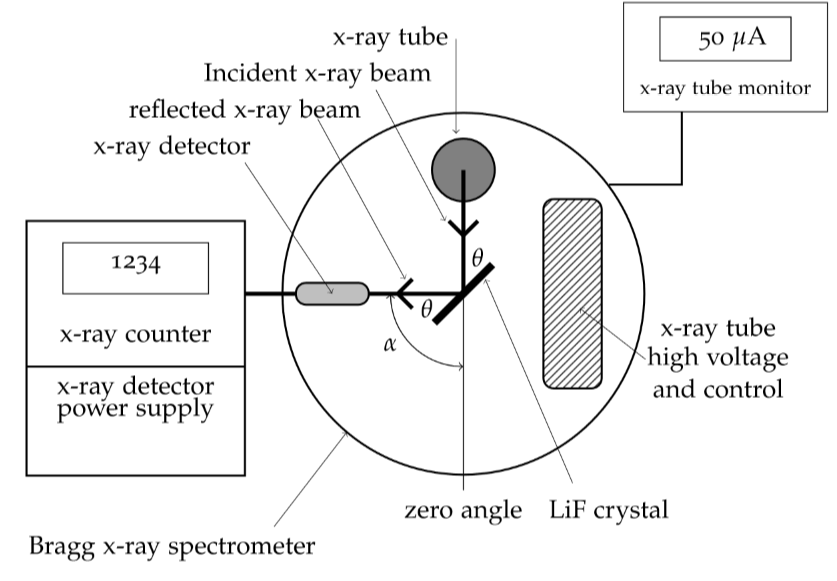
\includegraphics[scale = 0.8]{Images/XR8.PNG}
    \caption{An example of a typical Bragg x-ray spectrometer.}
    \label{fig:XR8}
\end{figure}

\noindent An x-ray tube generates a beam of x-rays. The x-ray tube is operated by an associated high voltage power supply together with control and monitoring electronics. The x-ray beam strikes a mounted crystal at some incident angle $\theta$. Bragg diffraction suggests that the reflected x-rays at the same angle $\theta$ will be at the single x-ray wavelength given by Bragg’s law, Equation \ref{eq:XR6}. The reflected beam is detected by an \Emph{x-ray detector}. An x-ray detector measures the intensity of the reflected beam. Usually this is done by counting the number of arriving x-ray photons. The x-ray detector also requires its own power supply and control system.

\noindent The apparatus is arranged so that the detector can be rotated to any angle $\alpha$. An internal mechanism links the rotation of the detector to the rotation of the crystal. This is done so that for any detector angle, $\alpha$, the crystal is positioned such that the angle of incidence, $\theta$, equals the angle of reflection, $\theta$, as seen in Figure \ref{fig:XR8}. The angle $\alpha$ is always twice the angle $\theta$ so that \begin{equation}\label{eq:XR7}
    \alpha = 2\theta
\end{equation}
In this way the number of x-rays at any wavelength is determined and when the resulting data is plotted, an x-ray spectrum such as the one in Figure \ref{fig:XR4} is obtained. The crystal spacing and Equation \ref{eq:XR6} canthen be used to relate an x-ray wavelength to each angle. Equation \ref{eq:XR6} also suggests that higher order spectral features may be visible when $n = 2, 3, ... $. In general, higher order spectra are less bright (a smaller number of x-ray photons) than the primary ($n = 1$) spectrum because the extra travel distance through the crystal increases the probablity that the x-ray photon will be absorbed inside the crystal. A more detailed view of the Bragg spectrometer actually used in this experiment is shown in Figure \ref{fig:XR9}. The most significant addition to the instrument are \Emph{safety interlocks and shielding}. Due to their penetrating nature, x-rays are considered to be harmful radiation when received in large doses. For this reason, practical x-ray spectrometers are shielded and are equipped with interlocks so that it is impossible to operate the instrument when the shielding is removed. The first layer of shielding is a \Emph{dome shield} completely surrounding the x-ray tube and made of leaded glass. An \Emph{aperture slit} is mounted in this shield so that a narrow beam of x-rays can escape and strike the diffraction crystal mounted at the center of the x-ray spectrometer. The second layer of shielding are the two lead slits (the \Emph{entrance slit} and \Emph{collimating slit}) that block the diffracted xrays from escaping the instrument, except for a narrow beam that is permitted to reach the detector. The angular resolution of the x-ray spectrometer is determined by the width of these two slits and the distance between them. The third layer of shielding is the \Emph{detector tube} and \Emph{detector socket} assembly which absorbs most of the remaining x-rays in the diffracted beam. The fourth layer of shielding is the cover of the instrument. The spectrometer interlocks are designed so that the x-ray tube cannot be energized unless the cover is closed and properly centered. The fifth and final layer of shielding is the \Emph{aluminum and lead backstop} that blocks the remaining portion of the direct non-diffracted portion of the x-ray beam. Under normal operation with these safeguards in place, the x-ray spectrometer used in this experiment has been certified as radiologically safe for educational use.

\begin{figure}[H]
    \centering
    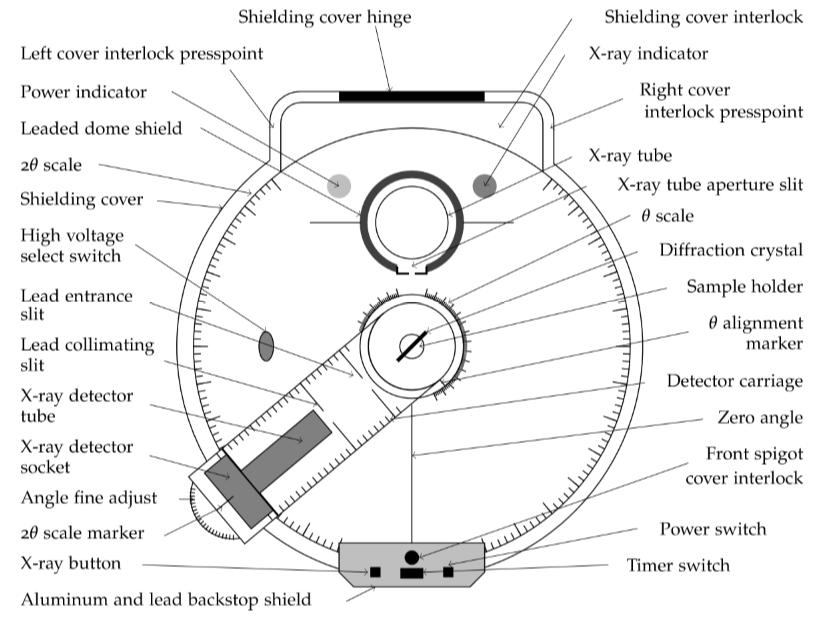
\includegraphics[scale = 0.8]{Images/XR9.PNG}
    \caption{ A detailed view of the Bragg spectrometer used in this experiment.}
    \label{fig:XR9}
\end{figure}

\noindent The x-ray spectrometer shown in Figures \ref{fig:XR8} and \ref{fig:XR9} can be used to experimentally examine both the production of x-rays by the x-ray tube and the diffraction of x-rays by the sample cystal mounted in the instrument. The x-ray tube used in this experiment has a copper target anode. So it is expected that the K-shell peaks visible in the spectrum should originate from copper atoms and have the characteristic energies of copper. The x-ray tube is operated at a voltage of $30 \;kV$ and would be expected to produce a bremsstrahlung spectrum with a cut-off as specified by Equation \ref{eq:XR2} if the theory of braking radiation is correct. The crystal used to diffract the x-rays is lithium fluoride. The density of LiF can be used to deduce the atomic spacing of this crystal assuming a cubic structure. The Bragg spectrometer can then be used to measure the spectrum emitted by the x-ray tube by moving the detector to different angles and recording the x-ray photon count at each angle. Bragg’s law relates the detector angle to the x-ray wavelength assuming the atomic structure of the crystal is understood. Analysis of the x-ray spectrum allows to test Bragg’s law and the theory of x-ray production and measurement. Lastly, bremsstrahlung can be further examined by placing a thin piece of plastic in the x-ray beam. If the reason for the long low energy tail is due to x-ray absorption, then a piece of plastic should attenuate the low energy part of the spectrum to a much greater extent than the high energy portion. This can be checked by comparing x-ray spectra with and without the plastic against each other.


\noindent As is common in spectroscopy, there is a dilemma between accepting the properties of the diffraction grating (in this case a crystal) or accepting the properties of the light source (in this case an x-ray tube). If the grating is trusted, then the grating can be used to measure the spectrum of the incoming x-rays. If the x-ray tube is trusted, then the x-ray beam can be used to examine the atomic structure of the sample being irradiated. In this experiment, neither device is treated as the accepted standard. Instead, the accepted values for the atomic spacing of LiF, the $K_{\alpha}$ and $K_{\beta}$ wavelengths of copper, and the bremsstrahlung cutoff are compared with the measured values to establish the consistency of the x-ray spectrometer system with x-ray theory. In practice independent evidence is gathered to establish the behaviour of x-ray spectrometers. The structure of LiF is independently deduced by the known chemical properties of ionic solids and the fracture properties of LiF crystals. The wavelengths of x-rays are independently verified without crystals by using ruled gratings that are tilted nearly horizontally to effectively decrease the line spacing of the grating to the point where x-ray diffraction can be obtained.

\section{Experimental Procedure}

\begin{itemize}[leftmargin = 50pt]
    \item[Step 1:] The apparatus is connected together as shown in Figure \ref{fig:XR8}. Make sure all instruments are turned off before proceeding. The x-ray spectrometer is a nearly self-contained unit except for the x-ray counter and the tube current monitor. The x-ray detector cable should be connected to the GM tube input connector on the right on the Tel-Atomic Digicounter. The monitor tube current output should be connected to the current jacks on the digital multimeter with the supplied cable. Set the multimeter to a range compatible with a current on the order of $50 \;\mu A$ DC.
    \item[Step 2:] The Tel-Atomic Digicounter powers the x-ray detector tube and accumulates and displays the detected x-ray photon counts. For consistent repeatable operation, that enables comparisons between different instruments, the following settings are recommended. The GM Tube Supply voltage should be $420\; V$. The counting switch should be set to continuous and the function switch turned to radioactivity. Adjust the range switch to $10\;s$. Set the timing switch to stop and the Triggered setting to off. The remaining switches and connections can be neglected.
    \item[Step 3:] The following checks and configurations are recommended for proper operation of the x-ray spectrometer. The names of the various spectrometer parts as used here are shown in Figure \ref{fig:XR9}. First lift the spectrometer cover (shielding cover). This cover has an interlock, so there is a special procedure for opening it. As seen in Figure \ref{fig:XR9}, there are cover interlock presspoints on both sides of the spectrometer at the back. To open the cover, press the right interlock presspoint to shift the entire cover left. The cover can be opened once the cover is shifted fully leftwards. The cover hinge is at the rear, so it is opened by reaching under the backstop shield and raising the opening from the front. Once the cover is lifted, examine the instrument. Do \Emph{NOT} touch the crystal, it is brittle and sensitive to moisture, but check that it is present, centered in the sample holder, and the top of it has a dab of blue paint. The blue paint identifies the crystal as LiF. Make sure the x-ray tube is installed and fully covered by the leadglass dome shield. Inspect the backstop shield to make sure there is a thin plate of lead behind the plate of aluminum on the outside of the cover. Set the high voltage select switch to $30 \;kV$. Check that a $1\;mm$ lead aperture slit is installed at the exit port of the x-ray tube. Note that the carriage holding the detector has numbered slots. A $1 \;mm$ lead collimator should be present in slot 13 of the detector carriage and a $3\;mm$ lead collimator should be installed in slot 18. Lastly, the x-ray detector itself should be installed in slot 26 of the detector carriage.
    \item[Step 4:] Check that the detector carriage moves freely between $20^{\circ}$ and $120^{\circ}$ on the $2\theta$ scale. For proper operation, the detector carriage must always be on the left side of the instrument as seen in Figures \ref{fig:XR8} and \ref{fig:XR9}. The reason for this is that the crystal has a preferred face where it has been carefully cleaved, and this is the side that should be exposed to the x-ray beam. Verify that the mechanism which rotates the crystal is working correctly. To do this, rotate the detector and, if possible, compare the reading on the $2\theta$ scale with the reading on the $\theta$ scale. One should be double the other. The $2\theta$ scale is read by the scale marker just behind and underneath the detector socket. The $\theta$ scale is read by the angle alignment marker line that is visible on the ring surrounding the sample holder. Next, check the zero alignment of the spectrometer. This is done by rotating the detector to $0^{\circ}$ on the $2\theta$ scale. When the zero alignment is correct, the $\theta$ scale should also be registering $0^{\circ}$ at this point. If there is a misalignment, contact the laboratory staff
    \item[Step 5:] At this point the instruments are ready to be turned on and the interlocks on the spectrometer checked. Lower the lid and center it using the left and right interlock presspoints. The cover is correctly centered when the front spigot interlock is centered on the the zero angle line. Check (gently) that the cover cannot be opened when it is centered at this position. Turn on the power to the Digicounter and the multimeter. To power up the spectrometer, rotate the timer switch clockwise to the 50 minute mark and then turn on the power switch. The power indicator should light up and the filament inside the x-ray tube should begin to glow. Then press the x-ray button. If the cover is correctly centered, the x-ray indicator should light up and the spectrometer will begin generating x-rays. If the x-ray indicator does not light, it usually implies that the cover needs a minor position readjustment. Once turned on, check the interlock by pressing the right interlock presspoint and shift the lid left. The x-ray indicator should immediately turn off if the interlocks are operating properly. Re-center the cover and turn the x-rays back on. Report to your laboratory instructor and the laboratory staff if the interlock system is not working correctly.
    \item[Step 6:] Let the x-ray system warmup and stabilize for about fifteen minutes. Monitor the beam current on the multimeter during this time. The accepted range of operation for the x-ray tube is a beam current between $30$ and $70 \;\mu A$.
    \item[Step 7:] The spectrometer is now operational. Obtain an x-ray spectrum. At each degree for $2\theta$ between $20^{\circ}$ and $120^{\circ}$ record the ten second x-ray photon counts. The Digicounter automatically repeats ten second measurements so the reset button on the Digicounter is not required. It is sufficient to make sure that a full ten second measurement is made at each angle before moving the detector onto the next angle. Occasionally check the timer switch, and when it nears zero, again turn the time clockwise back up to 50 minutes. For best results keep the spectrometer running continuously for the entire acquisition of the spectrum. The best practice is to adjust the dial to maximum of 50 minutes every 30 minutes, for ``fool proof" operation.
    \item[Step 8:] Insert a plastic plate in a slot between the two collimators on the detector carriage and obtain a second spectrum in the same manner as the first spectrum.
    \item[Step 9:] Once the second spectrum is completed, turn off the spectrometer and the other instruments.
\end{itemize}


\section{Error Analysis}

It might be expected that an x-ray spectrum obtained with the Bragg spectrometer used in this experiment would have an appearance something like that shown in Figure \ref{fig:XR4}. This suggests that the x-ray spectra obtained in this experiment are actually graphs of x-ray photon counts versus angle, where the $2\theta$ detector angle is the independent variable and, $N$, the number of x-rays, is the dependent variable. As with any graph made from measurements, there will be error bars on each data point reflecting the uncertainty with which it was obtained.

\noindent In this experiment, the uncertainty in the angle is dominated by the width of the x-ray beam passing through the instrument. The width of the x-ray beam is determined by the widths and separations of the lead slits in the apparatus. An estimate of the beamwidth can be found by sighting through all of the slits while moving the detector carriage and observing how much the detector must move to each side before the anode of the x-ray tube is blocked. For the instrument used here, it is found that the beamwidth is $3^{\circ}$ on the $2\theta$ scale. So the error in $2\theta$ is $1.5^{\circ}$ and the error in $\theta$ would be at least half of this. Since there are also alignment errors between rotations of the crystal and rotations of the detector, rounding up the error to the nearest degree seems to be prudent. So a reasonable value to use for $u(\theta)$ would be $1^{\circ}.$

\noindent Additionally, due to the difficulty in observing angles between the physical lower limit of the spectrometer, $2\theta=18^{\circ}$, and the regime of easily measureable angles, $2\theta \geq 20^{\circ}$, uncertainties in these small-angle measurements should be chosen appropriately.


\noindent The detection of x-rays is a statistical process.  Each x-ray photon has a particular probability of being counted by the detector. For this reason, the number of x-rays counts varies, even when the angle remains unchanged. If the x-ray count measurement were repeated a large number of times at each angle, a distribution would be obtained, and the width of the distribution would be a good estimate of the error in the x-ray photon count. However, it is known that for photon counters, the distribution typically is gaussian at large count rates and poissonian at small count rates. In either case, a good estimate of the photon count error, $u(N)$, for both of these statistical distributions is \begin{equation}\label{eq:XR8}
    u(N) = \sqrt{N}
\end{equation}

\noindent Other sources of systematic error are also present. The precision with which the atomic spacing, d, is known affects the precision with which the x-ray wavelengths can be calculated from Bragg’s law. Moreover, the purity, quality, and uniformity of the crystal are large factors in the sharpness of the observed features in the x-ray spectrum. If the spacing of the LiF atoms is not identically cubic due to impurities or imperfections, then the analysis of Bragg x-ray diffraction as presented here does not fully apply. Lastly, the photons counted by the x-ray detector do not all originate from the x-ray tube. Other radioactive sources such as cosmic rays and trace amounts of isotopes in the spectrometer and surroundings contribute as well. These extra sources of photons are called background radiation. For this experiment, errors in the crystal lattice spacing and background radiation can be neglected.


%%%%%%%%%%%%%%%%%%%%%% Chapter 1.6
\chapter{Spectroscopy}


\begin{figure}[H]
    \centering
    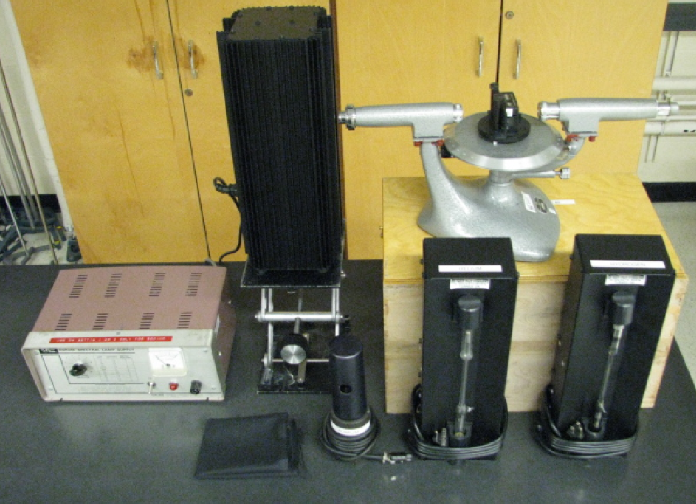
\includegraphics[scale = 0.8]{Images/SPEC1.PNG}
    \caption{Equipment used in the spectroscopy experiment.}
    \label{fig:SPEC1}
\end{figure}


\section{Background}

\subsection{The Spectroscope}

Spectroscopy is the study of the electromagnetic spectrum and the emission and absorption of electromagnetic radiation. The science of spectroscopy is useful in many areas that requires the analysis of light. Astronomers use spectroscopy to determine the composition of stars and galaxies. Much of what is known about the Sun comes from the analysis of its spectrum. One of the first to study the Solar spectrum was Joseph von Fraunhofer. In 1814 he found that the spectrum of the Sun contained fine, dark lines which, are now known to be caused by the absorption of light by gases in the Sun. A pattern of dark lines in a continuous spectrum is called an \Emph{absorption} spectrum. In contrast, discrete coloured lines on a dark background is called an \Emph{emission} spectrum and is caused by the emission of light by excited atoms.

\noindent The spectral lines visible to the human eye vary from violet to red in colour. The most common method of studying spectra is through the use of a \Emph{spectroscope}. This type of instrument enables the user to observe the spectrum of various elements and facilitates the measurement of the wavelengths of each spectral line. Figure \ref{fig:SPEC2} shows a schematic diagram of the Introductory Student Spectroscope used in this experiment. Light passes through the \Emph{slit} and the \Emph{collimator}, a device producing a parallel beam of rays. It is then bent by the \Emph{diffraction grating}. The \Emph{telescope} is connected to a rotatable arm so that it can be moved to allow the diffracted light to pass through it. A vernier on the telescope is then used to measure the angle at which the incident light is diffracted. Then this angle can be used to find the wavelength of the selected emission line. Encircling the base of the grating table is a $360$ degree scale used to make measurements in conjunction with the vernier scale, which is fixed to the telescope arm.

\begin{figure}[H]
    \centering
    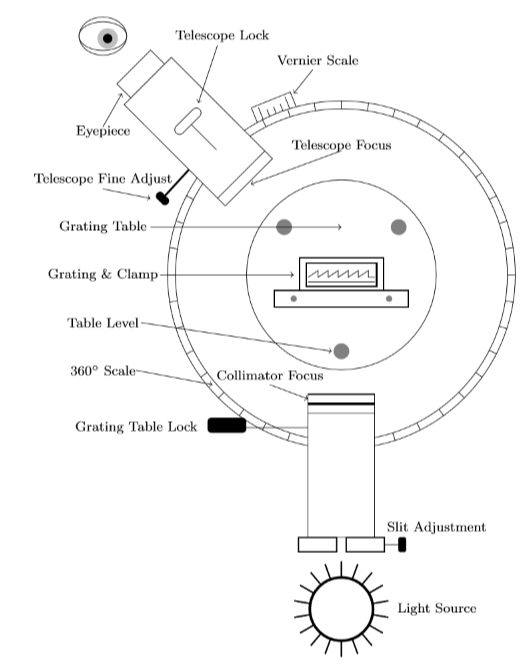
\includegraphics[scale = 0.8]{Images/SPEC2.PNG}
    \caption{A diagram of the spectrometer used in this experiment.}
    \label{fig:SPEC2}
\end{figure}

\noindent Before the spectroscope can be used to measure the angles of spectral lines it must be adjusted to ensure that accurate results are obtained. To begin, the telescope is focused on a distant object, using the \Emph{telescope focus}. The telescope is then lined up with the slit in the end of the collimator, and the \Emph{collimator focus} is adjusted until the slit comes into sharp focus. In this way only approximately parallel rays of light pass through the \Emph{diffraction grating}.

\subsection{Diffraction Gratings}

A diffraction grating can be imagined as a flat surface with thousands of grooves. As seen in Figure \ref{fig:SPEC3}, the diffraction grating used in this experiment has a sawtooth pattern, called a \Emph{blazed grating}, instead of simple grooves.

\begin{figure}[H]
    \centering
    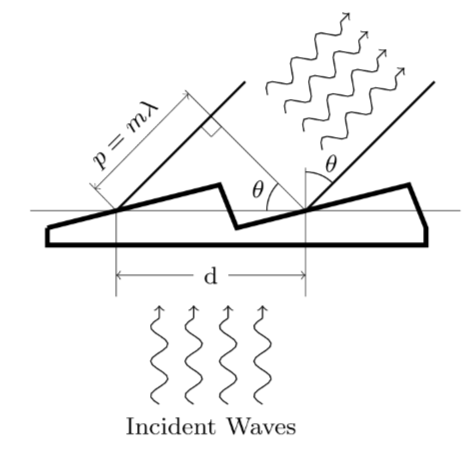
\includegraphics[scale = 0.8]{Images/SPEC3.PNG}
    \caption{Diffraction of incident light by grating.}
    \label{fig:SPEC3}
\end{figure}

When light from an emission spectrum passes through a blazed diffraction grating the light is split into its constituent colours. Atomic spectra are observed as a series of lines because of the constructive interference of the light waves once they have passed through the diffraction grating. Destructive interference produces what is observed between spectral lines. Constructive interference occurs when two or more waves of light, of equal wavelength, are superimposed in phase, resulting in a maxima, or a spectral line. In order for two identical light waves, diffracted by side by side grooves, to be in phase they must travel a distance that differs by one wavelength after they have been diffracted. As seen in Figure \ref{fig:SPEC3}, this implies that the distance, $p$, must be an integer multiple of the wavelength. Therefore, for constructive interference the requirement is that: \begin{equation}\label{eq:SPEC1}
    d\sin\theta = m\lambda, \;\;\;m = 0,\pm 1,\pm 2,...
\end{equation}
where $d$ is the \Emph{line spacing}, that is, the distance from one point on a groove to the same point on the neighboring groove. Note that the number given on the top of the diffraction grating is the \Emph{line density}, not the line spacing. Line density is the inverse of line spacing. The \Emph{angle of deviation}, $\theta$, is the angle between the central maximum and the spectral line. The variable $m$ indicates the \Emph{order} of the spectral lines. First order spectral lines $(m = \pm 1)$ are those found closest to the central maximum. As the telescope arm moves away from the central maximum, a point is reached where the spectral lines begin to repeat. These are known as the second order spectral lines $(m = \pm 2)$. ALthough second order maxima are visible, only first order maxima are used in this experiment. The sign of the order is positive or negative depending whether the spectrum is to the right or left of the central maxima. Equation \ref{eq:SPEC1} can be used to calculate the wavelength of a particular spectral line from the angle of deviation. For example, assuming a line spacing of $1000\;lines/mm$ and a first order angle of deviation of $30^{\circ}$ a wavelength of $500\;nm$ is calculated.

\subsection{Spectral Sources}

The light from the emission spectrum that passes through the diffraction grating is generated by lamps called \Emph{spectral sources}. Three different types of spectral sources are used in this experiment: the Geissler tubes, the low pressure lamps, and the gas discharge tubes. In general, the glass parts of spectral lamps should not be touched. Touch only the metal ends of the tube. After a lamp is turned on move it as little as possible so that its lifetime is not shortened. When finished with a light source allow the lamp to cool for at least five minutes before moving it. Once a tube is removed from the set up, store it away immediately before starting to use a different tube.

\noindent The Giessler tubes (like the Hydrogen one) are constructed by filling a glass tube with a pure sample of the desired gas and then adjusting the pressure of the gas to yield maximum brightness. The glass tube is fitted with two electrodes, one at each end. The completed tube is clamped into a high voltage power supply. The high voltage creates an electric field between the electrodes which causes the valence electrons in the atoms to become excited. When the excited electrons lose energy they give off a mixed light containing all wavelengths that are characteristic of the element contained in the tube. Geissler spectral lamps should be turned off when not being used to lengthen their life. Be careful when handling a high voltage supply, do not touch any exposed metal parts.

\noindent The low pressure tubes contain a source that is solid at room temperature so there is insufficient vapour present for the lamp to be started at any reasonable voltage (less than several thousand volts). It was found that by adding a noble gas mixture to the lamp (usually Argon and Neon, in various proportions), the starting voltage could be lowered to about $600$ Volts. When a cold lamp is turned on a voltage ``kick" is supplied to the discharge tube which generates enough charge carriers that the Argon and Neon become conductive. Once conduction begins, the voltage decreases and the discharges remain confined to the noble gases. As the noble gases discharge, heat is generated which eventually causes the source to vaporize. The vaporized atoms are excited by the electric field present in the lamp. The noble gases are not excited any more because the valence electron of the source is much easier to excite that any of the electrons in the noble gases. When using the low pressure lamp it is important to allow the lamp to warm up for at least ten minutes before making any measurements in order to ensure that the spectrum being measured is actually that of Sodium and not of Neon or Argon. The low pressure lamp should be left until all measurements are completed. Turning the lamp on and off will reduce its lifetime, and it is also time consuming as the lamp must be warmed up each time it is turned on.

\subsection{The Hydrogen Atom}

One of the most commonly studied emission spectra is that of Hydrogen. With the simplest spectrum, Hydrogen is the most basic case of emission and absorption to study. Excited atoms can emit electromagnetic radiation at many wavelengths but for the purposes of this experiment, only the visible region of the electromagnetic spectrum is examined. The visible emission spectrum of Hydrogen is known as the \Emph{Balmer Series}, named after Swiss mathematician who first discovered their pattern.

\noindent Johann Balmer (1825-1898) was a secondary school mathematics teacher. As an adept mathematician, Balmer was able to produce a formula that predicts the wavelength of Hydrogen spectral lines with great accuracy. His empirical \Emph{Balmer formula} takes the form: \begin{equation}\label{eq:SPEC2}
    \frac{1}{\lambda} = R\left[\frac{1}{2^2} - \frac{1}{n^2}\right],\;\;\;n=3,4,5,...
\end{equation}
where $R$ is now called \Emph{Rydberg's constant} and each integer $n$ corresponds to an observed Hydrogen spectrum line. A proper explanation was not available until the Danish physicist, Niels Bohr (1885-1962) provided his theory of the atom which demonstrated that \begin{equation}\label{eq:SPEC3}
    R = \frac{m_ee^4Z^2}{8\varepsilon_0^2h^3c}
\end{equation}
where $Z$ is the atomic number of the atom.

\section{Experimental Procedure}

\begin{itemize}[leftmargin = 50pt]
    \item[Step 1:] Remove the diffraction grating and its holder from the spectroscope. It is extremely important not to touch any of the lenses or the diffraction grating. Do not use fingers or articles of clothing to clean the optical equipment as this will only result in scratching the optics. Hold the diffraction grating by its frame.
    \item[Step 2:] The telescope must be focused for parallel light rays and the crosshairs must be put into focus. First slide the eyepiece on the telescope in or out and bring the crosshairs into shapr focus. Next, focus the telescope on a distant object across the room or out a window. (Remember to rotate the telescope to avoid trying to focus through the collimator)
    \item[Step 3:] Use the Hydrogen lamp as the calibration light source and place it so that the light from it passes through the slit in the collimator. Aim the telescope at the slit and gently move the lamp until the slit is at its brightest. Adjust the collimator focus until the slit is in sharp focus. In this way the spectrum being measured uses only light parallel to the slit. Align the cross-hairs in the eyepiece with the slit. Do not change the focus of the telescope or the collimator, or rotate the eyepiece for the remainder of the experiment, as this affects the apparent position of the centre slit. Do not move the telescope by touching the eyepiece or the chrome part of the telescope, as this could change the focus of the telescope.
    \item[Step 4:] Replace the diffraction grating into its holder. The bolts for the diffraction grating holder should be facing the collimator, and the diffraction grating frame should be placed in the holder so that the diffraction grating is as close to the holder as possible. The idea here is that the diffraction grating needs to pass through the centre of the grating table as seen in Figure \ref{fig:SPEC2}
    \item[Step 5:] Turn the telescope and look at spectral lines that are far away from the center angle (choose second order lines if possible). Using the three grating table leveling screws on the bottom of the grating table, adjust the level of the table until the lines are vertically in the middle of the telescope as shown in Figure \ref{fig:SPEC4}. Move the telescope to the other side of centre and adjust the lines until they are also centered. This adjustment may have to be repeated several times on each side.

\begin{figure}[H]
    \centering
    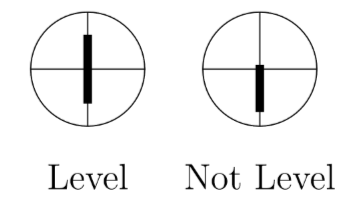
\includegraphics[scale = 0.8]{Images/SPEC4.PNG}
    \caption{Levelling the grating table.}
    \label{fig:SPEC4}
\end{figure}
    \item[Step 6:] Look through the telescope and adjust the width of the slit. Take note of which side of the slit moves. All measurements should be taken from the side of the light line that does not move. By doing this the width of the slit can be changed during the experiment. The slit width adjustment is used to adjust the amount of light that is allowed to pass into the collimator, as different amounts of light are useful in different situations. Some lines are close together and will overlap if the slit is too wide, in which case a narrow slit is required in order to resolve all of the lines that are present. On the other hand some lines are very dim. In such a case a wide slit is better in order for the spectral line to be bright enough that it can be seen.
    \item[Step 7:] Align the diffraction grating so it is perpendicular to the collimator as seen in Figure \ref{fig:SPEC3}. This is done by rotating the grating table. If the diffraction grating is not perpendicular, the angle of deviation of the spectral lines will differ between the two sides of the centre maximum. Choose any line in the spectrum and rotate the grating until the angle of deviation is the same on the left spectrum as the right spectrum. This step may need to be repeated several times.
    \item[Step 8:] Measure the angle of the centre maximum. Align the cross-hairs with the stationary edge of the slit. Use the vernier to measure the angle of the maximum. All angles of diffraction are measured with respect to this centre angle. Each angle of diffraction is subtracted from the centre angle and the absolute value of that angle is the angle of deviation. The angle of deviation is then used to determine wavelengths of spectral lines using Equation \ref{eq:SPEC1}.
    \item[Step 9:] Use the Hydrogen spectral lamp to check the performance of the diffraction grating. Measure the angle of deviation on both sides of the maximum for the four lines calculated according to the Equation \ref{eq:SPEC2}. The measured angles of deviation, along with Equation \ref{eq:SPEC1}, can be used to calibrate the spectroscope. If Equation \ref{eq:SPEC1} holds, a plot of $\lambda$ versus $\sin\theta$ should yield a straight line with slope $d$ and an intercept of zero.
    \item[Step 10:] Using wavelengths calculated using Equation \ref{eq:SPEC2} and measured angles of deviation, make a quick plot of $\lambda$ versus $\sin\theta$ (errors need not be included here). Check that the slope of this line corresponds to approximately $600 \;lines/mm$.
    \item[Step 11:] The spectroscope is now adjusted, checked, and ready for analyzing other spectra. Turn on one of the unknown sources and shine the light through the slit in the collimator. Measure the angles of deviation, on both side of the center maximum, for the visible lines.
    \item[Step 12:] Repeat these measurements for the other two spectral lamps. Remember, that these lamps have to be warmed up before you can start the measurements.
\end{itemize}

\section{Error Analysis}

Usually $u(\theta)$ would be half the smallest division of the vernier on the spectroscope, however there are other factors that add to the error. First, it is hard to take measurements from the same part of the spectral line each time a measurement is made. Second, as the eye moves back and forth across the eyepiece the cross-hairs move, therefore in order to get precise measurements the eye would have to be in exactly the same place for each measurement. Third, some lines are not very intense making them hard to see, and lining the cross-hairs up becoms difficult. Fourth, the cross-hairs have a thickness which introduces an uncertainty in any visual measurement. Fifth, the condition of the grating, i.e., smudges, scratches, etc., can introduce visual abberrations like smearing. Finally, the spectroscope and diffraction grating used cannot distinguish between spectral lines that are too close together. This is a limitation of the diffraction grating construction as well as the magnification of the telescope. For example, the lines of the Sodium doublet differ by about half a nanometer and they are very close to appearing as one line. For these reasons, take the error in measurements of angles for this spectroscope to be $0.2^{\circ}$. For the uncertainty in the line density of $600\;lines/mm$ for the diffraction grating a value of $5\;lines/mm$ has been found to be reasonable to use for the diffraction grating check. For other the line density and error determined by the grating performance check can be used. Note that $u(\theta)$ must be in radians when calculations are being made. All other errors should be propagated using an appropriate method.



%%%%%%%%%%%%%%%%%%%%%% Chapter 1.7
\chapter{Voltage Dividers and Sources}


\begin{figure}[H]
    \centering
    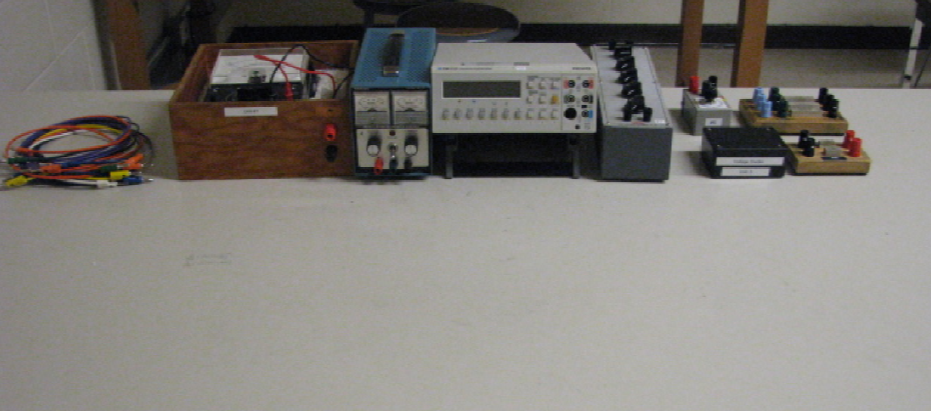
\includegraphics[scale = 0.8]{Images/Divid1.PNG}
    \caption{Equipment used in the DC Circuit Experiment}
    \label{fig:DCSetup}
\end{figure}

\section{Background}

In almost all circuits \Emph{resistors} are among the most common components. Figure \ref{fig:DC2} shows some of the many different kinds of resistors. The different shapes and sizes play a role in their behaviour and application. Resistors are used to control the current and voltage in a circuit.

\begin{figure}[H]
    \centering
    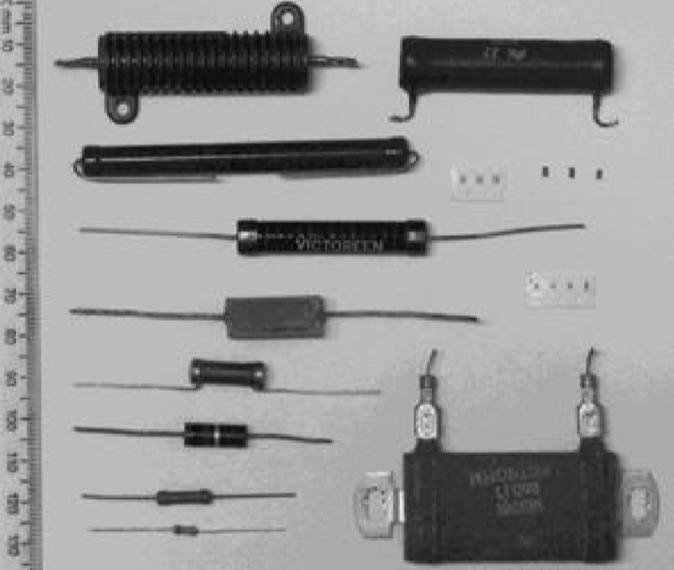
\includegraphics[scale = 0.8]{Images/DC2.PNG}
    \caption{Examples of resistors of different shapes and sizes.}
    \label{fig:DC2}
\end{figure}

Georg Ohm (1789-1854) contributed largely to what is now known about resistors. He speculated how current might work and formulated the law governing resistors that now bears his name. Later, Gustav Kirchhoff (1824-1887) made further contributions to understanding of electric circuits. He extended Ohm's work describing what are now called \Emph{Kirchhoff's Laws}, which explained how current and voltage in electric circuits are related. In 1883 L\'{e}on Th\'{e}venin (1857-1926), a french telegraph engineer, described what he thought to be a new theory of equivalent circuits. He showed that any resistor circuit could be simplified to make analysis easier. Coincidentally, the concept of equivalency in circuits had already been proposed almost 30 years earlier by the physicist Hermann von Helmholtz (1821-1894). Th\'{e}venin was unaware of Helmholtz's work and both theories met with resistance during their time. It was due to Th\'{e}venin's engineering approach, and the growth of electrical engineering in the coming years, that his result is now called Th\'{e}venin's Theorem.

\noindent Many combinations of resistors exist in circuitry, but the \Emph{voltage divider} is one combination that is seen everywhere. The circuit in Figure \ref{fig:DC3} contains a voltage source of some kind, connected in series with two resistors. A voltmeter is in parallel with one of the resistors to measure the voltage across it. Each resistor in the loop drops a portion of the voltage. This resistor combination, which accomplishes the splitting of voltages, is called a voltage divider. It can be used to control the voltages coming out of, or going into, a particular system, or even be used as a tool for analysis of circuits.

\begin{figure}[H]
    \centering
    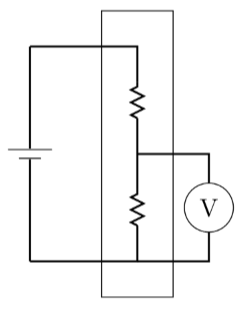
\includegraphics[scale = 0.8]{Images/DC3.PNG}
    \caption{Basic voltage divider with power supply.}
    \label{fig:DC3}
\end{figure}

\noindent In Figure \ref{fig:DC4} the connections of the voltage divider to the voltage course and voltmeter are explicitly shown. The voltage source is supplying a voltage with magnitude $V_{in}$ into the voltage divider, and the voltmeter reads $V_{out}$ across $R_2$. This suggests the voltage divider can be generalized further by extracting it from circuit

\begin{figure}[H]
    \centering
    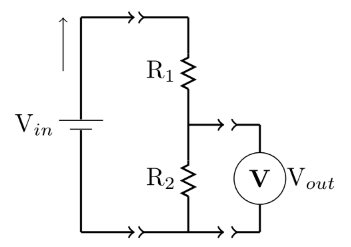
\includegraphics[scale = 0.8]{Images/DC4.PNG}
    \caption{Connections for the voltage divider to voltage source and voltmeter.}
    \label{fig:DC4}
\end{figure}

\noindent Figure \ref{fig:DC5} shows only the voltage divider. The input voltage, $V_{in}$, can be generalized to be any source of voltage such as a battery, power supply or another device. The output voltage, $V_{out}$, is what would be applied to any device or system connected to these terminals.

\begin{figure}[H]
    \centering
    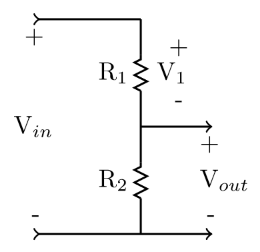
\includegraphics[scale = 0.8]{Images/DC5.PNG}
    \caption{Isolated voltage divider.}
    \label{fig:DC5}
\end{figure}


For the voltage divider in Figure \ref{fig:DC5}, $V_{in}$ is split and $V_{out}$ is some portion of $V_{in}$. This can be shown using Ohm's and Kirchhoff's laws. From Ohm's law, the voltage drop across an ohmic resistor is the product of its resistance and the current through it. So the voltages across $R_1$ and $R_2$ are $V_1$ and $V_{out}$, which are given by \begin{equation}\label{eq:DC1}
    V_1 = IR_1
\end{equation}
and \begin{equation}\label{eq:DC2}
    V_{out} = IR_2
\end{equation}
where $I$ is the current flowing in the loop. From Kirchhoff's Voltage Law, it is expected that the applied voltage equals the voltage drops across the resistors in series, so that \begin{equation}\label{eq:DC3}
    V_{in} = V_1 + V_{out}
\end{equation}

Using Equations \ref{eq:DC1}, \ref{eq:DC2}, and \ref{eq:DC3}, it is seen that \begin{equation}\label{eq:DC4}
    V_{in} = I(R_1+R_2)
\end{equation}
Substituting for the current using Equation \ref{eq:DC2} gives the \Emph{voltage divider formula}: \begin{equation}\label{eq:DC5}
    V_{out} = V_{in}\frac{R_2}{R_1+R_2}
\end{equation}
Equation \ref{eq:DC5} implies that the ration $\frac{V_{out}}{V_{in}}$ is equal to the ratio of $\frac{R_2}{R_1+R_2}$. It also implies that $V_{out}$ cannot be larger than $V_{in}$ since the ratio of one resistor to two resistors can only be equal to or less than one. A special case is when $R_1$ is zero. The ratio becomes equal to one and $V_{out}$ is equal to $V_{in}$,

\begin{figure}[H]
    \centering
    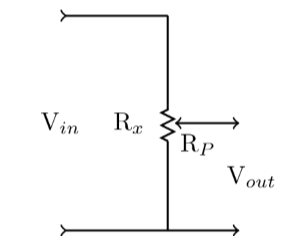
\includegraphics[scale = 0.8]{Images/DC6.PNG}
    \caption{Variable voltage divider.}
    \label{fig:DC6}
\end{figure}

The voltage divider in Figure \ref{fig:DC5} supplies a fixed voltage ratio. It is also possible for voltage dividers to supply a variable ratio. This is done with a device called a \Emph{ptentiometer}. A potentiometer is a variable resistor whose resistance can be changed by turning a dial. Figure \ref{fig:DC6} shows a schematic of a potentiometer used as a variable voltage divider. The resistance of the entire potentiometer is $R_x$ and $R_P$ is the portion of this controlled by the dial. If the dial is adjusted so that $R_P$ is equal to $R_x$, then $V_{out}$ is equal to $V_{in}$. Likewise $V_{out}$ becomes zero if the dial is adjusted so that $R_P$ is zero.

\noindent Suppose two more resistors are added to the potentiometer to get the circuit shown in Figure \ref{fig:DC7}. The derivation for Equation \ref{eq:DC5} involves a loop with two resistors, but in fact can work for any number of resistors. The total series resistance would be on the bottom of the ratio. The output voltage $V_{out}$ could be taken across any or all of the resistors in the circuit and the value of these resistors would go on the top of the ratio. So, the output voltage will be \begin{equation}\label{eq:DC6}
    V_{out} = V_{in}\frac{R_P+R_2}{R_1+R_2+R_x}
\end{equation}


\begin{figure}[H]
    \centering
    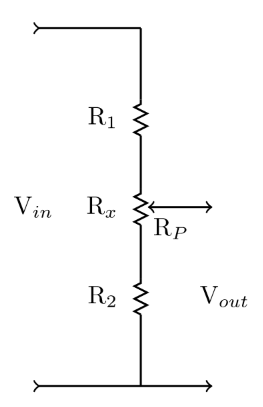
\includegraphics[scale = 0.8]{Images/DC7.PNG}
    \caption{Voltage divider with three resistors}
    \label{fig:DC7}
\end{figure}


This setup preoduces a range of voltages for $V_{out}$, which can be controlled by the dial on the potentiometer. THe output voltage has a minimum greater than zero and a maximum less than $V_{in}$, as determined by $R_1$ and $R_2$. The minimum output voltage, $V_{min}$, occurs when $R_P$ is zero so \begin{equation}\label{eq:DC7}
    V_{min} = V_{in}\frac{R_2}{R_1+R_2+R_x}
\end{equation}
and the maximum output voltage, $V_{max}$, arises when $R_P$ equals $R_x$ which gives \begin{equation}\label{eq:DC8}
    V_{max} = V_{in}\frac{R_x+R_2}{R_1+R_2+R_x}
\end{equation}
Not only do voltage dividers exist explicitly as the circuits shown in Figures \ref{fig:DC3}-\ref{fig:DC7}, they also exist implicitly whenever any two circuits are connected together. There is a division of voltages between the output of any circuit and the input of a secont circuit. For example, imagine that a single resistor is connected to a power supply as shown in Figure \ref{fig:DC8}. Here, the second circuit is composed of a single resistor $R_L$. Typically, $R_L$ is called the \Emph{load}, or in this case the \Emph{load resistor}.

\begin{figure}[H]
    \centering
    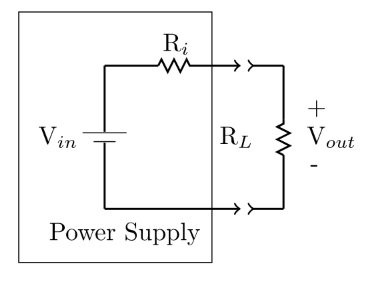
\includegraphics[scale = 0.8]{Images/DC8.PNG}
    \caption{Power supply with internal resistor.}
    \label{fig:DC8}
\end{figure}


Ideally, it would be expected that the entire voltage, $V_{in}$, would be developed across the load resistor. However, what happens in practice is that the voltage across the load, $V_{out}$, is always somewhat smaller than $V_{in}$. Moreover, the smaller the value of $R_L$, the larger the discrepancy between $V_{out}$ and $V_{in}$. This situation can be neatly explained by the addition of an internal resistor, $R_i$. THe voltage is now seen as being split between the load resistor $R_L$, and the internal resistor, $R_i$. The basic voltage divider formula, Equation \ref{eq:DC5}, can be used to find $V_{out}$ as before to get \begin{equation}\label{eq:DC9}
    V_{out} = V_{in}\frac{R_L}{R_L+R_i}
\end{equation}
What is now observable is that the voltage across $R_L$ is less than the voltage being supplied by the power supply. If $R_i$ is much smaller than $R_L$, $V_{out}$ is, to a reasonable approximation, equal to $V_{in}$. At the same time, if the value of $R_i$ is close to $R_L$, then $V_{out}$ will only be a portion of $V_{in}$. If $R_i$ were much larger than $R_L$ this effect would be dramatically increased and almost no voltage would be across $R_L$. For perfect power supplies $R_i$ is zero which means that $V_{out} = V_{in}$ for any load resistor. \begin{equation}\label{eq:DC10}
    \frac{1}{V_{out}} = \frac{R_i}{V_{in}}\frac{1}{R_L} + \frac{1}{V_{in}}
\end{equation}
With Equation \ref{eq:DC10}, $R_i$ can be found by connecting a variable load and measuring $V_{out}$ across different load resistances. It can be seen that plotting $\frac{1}{V_{out}}$ versus $\frac{1}{R_L}$ yields a straight line with slope $\frac{R_i}{V_{in}}$ from which $R_i$ can be found.

\begin{qst}
    What is internal resistance exactly?
\end{qst}

Th\'{e}venin answered this by showing that from the point of view of any resistor in a circuit, the rest of the circuit is equivalent to a voltage source with a series of internal resistances, just as in Figure \ref{fig:DC7}. For example, the left side of Figure \ref{fig:DC9} shows a circuit containing a number of voltage sources and resitors. From the point of view of a single resistor such as $R_5$, the entire remaining part of the original circuit is equivalent to a single voltage source in series with a single resistor, as shown on the right side of Figure \ref{fig:DC9}. This is called the Th\'{e}venin equivalent circuit. The voltage source, $V_{th}$, is called the Th\'{e}venin equivalent voltage and the resistor, $R_{th}$, is called the Th\'{e}venin equivalent resistance. Comparing this with Figure \ref{fig:DC8}, it is seen that the Th\'{e}venin equivalent circuit is a power supply with an internal resistance driving a load consisting of a chosen component, in this case $R_5$.

\begin{figure}[H]
    \centering
    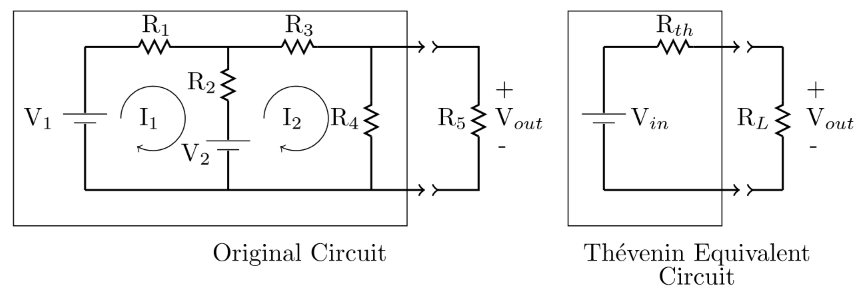
\includegraphics[scale = 0.8]{Images/DC9.PNG}
    \caption{Th\'{e}venin equivalent circuit.}
    \label{fig:DC9}
\end{figure}

There is a standard procedure for calculating $V_{th}$ and $R_{th}$. The Th\'{e}venin equivalent voltage is equal to the voltage that would be found across the terminals without anything attached to it. Here, $R_5$ is the reference component so it is placed with an open circuit. So the volrtage across $R_4$ is the voltage being output by this circuit and is equal to $V_{th}$. In this example the Th\'{e}venin voltage is equal to the product of the current in the second loop, $I_2$,a nd the resistance $R_4$. If the value for all the voltage sources and resistors are known, the current across $R_4$ can be found by solving for the loop currents. This will yield the Th\'{e}venin voltage as being \begin{equation}\label{eq:DC11}
    V_{th} = I_2R_4
\end{equation}
To find $R_{th}$, $R_5$ is again removed and all voltage sources in the circuit are replaced with their internal resistances. In this case the voltage sources are assumed to be the ideal and are replaced with short circuits. The Th\'{e}venin resistance is then the equivalent resistance at the open terminals. For the circuit in Figure \ref{fig:DC9} this is \begin{equation}\label{eq:DC12}
    R_{th} = ((R_1\;\vert\vert\;R_2)+R_3)\;\vert\vert\;R_4
\end{equation}
where $\vert\vert$ indicates the resistors are to be added in parallel.


\noindent Another way to measure $V_{th}$ and $R_{th}$ is by knowing that the Th\'{e}venin equivalent circuit in Figure \ref{fig:DC9} is identical to the circuit depicted in Figure \ref{fig:DC8}. Equation \ref{eq:DC10} can therefore be used to find the Th\'{e}venin voltage and resistance, $V_{th}$ and $R_{th}$, by varying the load resistance, $R_5$. Here, $V_{out}$ is the voltage across $R_5$, and $V_{in}$ and $R_i$ are $V_{th}$ and $V_{th}$ respectively. Again, plotting $\frac{1}{V_{out}}$ versus $\frac{1}{R_5}$ should yield a straight line. This method produces a graph giving $R_{th}$ and $V_{th}$ from the slope and intercept.


\noindent So by attaching a load resistor to a circuit, in the case of Figure \ref{fig:DC9} this was $R_5$, the voltage across the resistor is dependent on the internal resistance as explained by the voltage divider rule. The effect that a load resistor has on circuits is called \Emph{circuit loading}. Imagine the basic voltage divider in Figure \ref{fig:DC5} where a voltmeter is used to measure $V_{out}$. Just like the power supply, voltmeters have some internal resistance. In the analysis of Equation \ref{eq:DC5}, it was assumed that no current goes into the voltmeter, which is only true for an ideal voltmeter. The effect that non-ideal voltmeters have on voltage dividers is shown in Figure \ref{fig:DC10}

\begin{figure}[H]
    \centering
    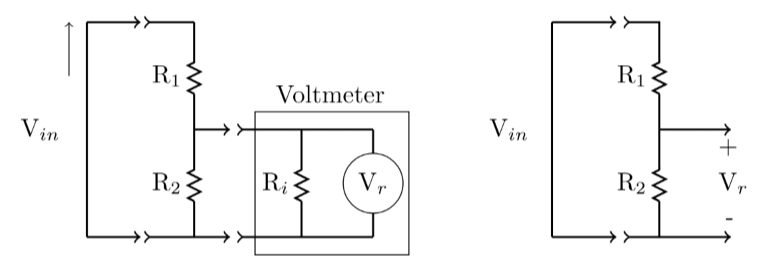
\includegraphics[scale = 0.8]{Images/DC10.PNG}
    \caption{Internal resistance of voltmeter.}
    \label{fig:DC10}
\end{figure}

This schematic is similar to Figure \ref{fig:DC4} with the expection that the voltmeter now has an internal resistance $R_i$. Ideally, the voltage acorss $R_2$ is the ratio fo $R_2$ to the entire resistance $R_1+R_2$. Once a voltmeter is connected, the voltage is split between $R_1$ and the combined resistance of $R_2$ and $R_i$, in parallel. In Figure \ref{fig:DC10}, $V_r$ is the voltage read by the voltmeter and $V_{out}$, although not explicitly shown, is the actual voltage across $R_2$ without the voltmeter attached. This equivalent resistance is given by \begin{equation}\label{eq:DC13}
    R_{eq} = R_2\;\vert\vert\;R_i = \frac{R_2R_i}{R_2+R_i}
\end{equation}
It is seen that if $R_i$ is much larger than $R_2$, then $R_{eq}$ is nearly equal to $R_2$, and Equation \ref{eq:DC5} still holds. This is what would be expected from an ideal voltmeter. If this is not the case then $R_{eq}$ will be smaller than $R_2$. So a larger portion of voltage will develop across $R_1$ than before the voltmeter was connected. The voltage measured by the voltmeter will now be smaller than expected. This effect is called \Emph{meter loading} and is seen when $R_2$ in Equation \ref{eq:DC5} is replaced with $R_{eq}$ to get \begin{equation}\label{eq:DC14}
    V_r = V_{in}\frac{R_{eq}}{R_{eq}+R_1} \neq V_{out}
\end{equation}
Equation \ref{eq:DC14} gives the output voltage, taking the effect of the voltmeter on the circuit into account. It can be used to calculate the internal resistance of the voltmeter. Furthermore, it is possible to rearrange Equation \ref{eq:DC14} to find the voltmeter internal resistance by \begin{equation}\label{eq:DC15}
    R_i = \frac{R_1R_2}{R_2\left(\frac{V_{in}}{V_r}-1\right)-R_1}
\end{equation}
If $R_1,R_2$ and $V_{in}$ are known, and $V_r$ is the reading from the voltmeter.

\noindent Two multimeters are used in this experiment, the Philips digital meter and the Sanwa analog meter. The Philips multimeter is close to ideal in many situations and is used for most of the measurements in this experiment. The Sanwa multimeter, which is farther from ideal, is used to see the effects of meter loading.

\noindent In this experiment the Philips multimeter is used for taking voltage and resistance measurements. All connections are made to the red V jack and the black COM jack. Switching between voltage and resistance readings is done via buttons along the bottom of the multimeter, under the display. The DC voltage function is selected by the V button and the resistance function is chosen with the 2W button. The three top right buttoms on the instrument are ranging controls. The range can be changed to automatic or manual with the AUT/MAN button. In manual mode the UP and DOWN buttons are used to change the range. Auto ranging is recommended unless otherwise specified. When measuring resistance be sure to disconnect any power supplies from the circuit. The internal resistance of the Philips voltmeter is $10$ M$\Omega$.

\noindent The Sanwa multimeter is an analog meter with a fairly low input resistance. This multimeter will be used to witness the effect of meter loading. The internal resistance of the Sanwa multimeter is directly proportional to the voltage range it is reading in and is $20\;k\Omega/V$.


\section{Experimental Procedure}


\begin{itemize}[leftmargin = 50pt]
    \item[Step 1:] Before constructing any circuits measure the resistance of all resistors using the Philips multimeter.
    \item Construct the basic voltage divider depicted in Figure \ref{fig:DC11} with $R_D = 100\;\Omega$ and $R_1 = 20\;\Omega$. Turn on the power supply and connect hte Philips multimeter across $R_1$ and take measurements of $V_{out}$ while changing $V_{in}$ from $1.0\;V$ to $5.0\;V$. 

        \begin{figure}[H]
            \centering
            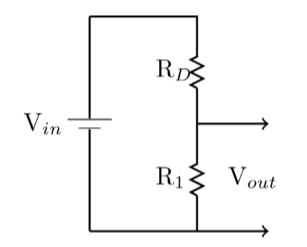
\includegraphics[scale = 0.8]{Images/DC11.PNG}
            \caption{Schematics of the basic voltage divider}
            \label{fig:DC11}
        \end{figure}
    \item[Step 3:] Measure the resitance of the potentiometer $R_x$ using the Ohmmeter across the red and black terminals. Build the circuit in Figure \ref{fig:DC12} with $R_D = 100\;\Omega$ and $R_1 = 20\;\Omega$. Set $V_{in}$ to approximately $1.0\;V$ and measure $V_{in}$ with the Phillips multimeter.
        \begin{figure}[H]
    \centering
    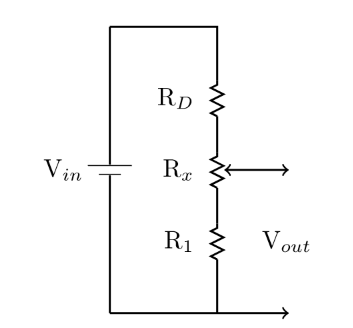
\includegraphics[scale = 0.8]{Images/DC12.PNG}
    \caption{Voltage divider with three resistors}
    \label{fig:DC12}
\end{figure}
    \item[Step 4:] Connect $R_D = 100\;\Omega$ to the positive output terminal of the power supply. This will show the effects of having a power supply with a high output resistance. Connect a resistance decade box in series to serve as a variable load. The setup should resemble Figure \ref{fig:DC8}. Set the power supply to $1.0\;V$. Using the Philips multimeter, take at least 10 measurements of $V_{out}$ while varying the load resistance from $10\;\Omega$ ot $10\;k\Omega$.
    \item[Step 5:] Remove $R_D$ from the circuit. Now $R_i$ is the actual internal resistance of the power supply to be measured. Repeat the measurements from Step 4.
    \item[Step 6:] Choose one of the circuits in Figures \ref{fig:DC13}-\ref{fig:DC14} and build it. Set the power supply between $1.0\;V$ and $5.0\;V$. Measure $V_{th}$ directly with a voltmeter. Replace the power supply with a short and measure $R_{th}$ directly with an ohmmeter. \Emph{Remember to disconnect the power from a circuit before taking measurements of resitance with an ohmmeter}.

        \begin{figure}[H]
    \centering
    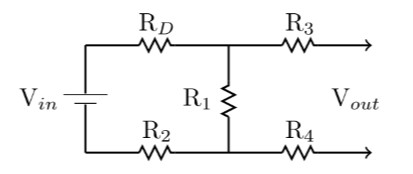
\includegraphics[scale = 0.8]{Images/DC13.PNG}
    \caption{Optional circuit diagram A}
    \label{fig:DC13}
\end{figure}
\begin{figure}[H]
    \centering
    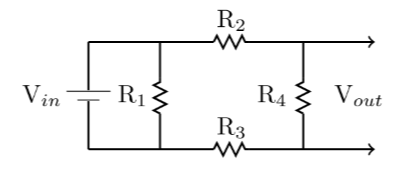
\includegraphics[scale = 0.8]{Images/DC14.PNG}
    \caption{Optional circuit diagram B}
    \label{fig:DC14}
\end{figure}
    \item[Step 7:] Cpmmect a resistance decade box across $V_{out}$ for the circuit chosen. This is the load resistor $R_L$ and creates a voltage divider between $R_{th}$ and $R_l$. Take at least 10 measurements of $V_{out}$ across the load resistor, as the resistance is varied from $10\;\Omega$ to $10\;k\Omega$. Equation \ref{eq:DC10} can then be used to deduce the Th\'{e}venin equivalent voltage and resistance.
    \item[Step 8:] Using resitance measurements only, deduce the contents of the box pictured in Figure \ref{fig:DC15}.

        \begin{figure}[H]
    \centering
    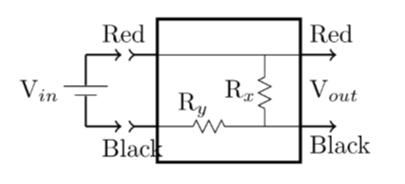
\includegraphics[scale = 0.8]{Images/DC15.PNG}
    \caption{Voltage divider black box}
    \label{fig:DC15}
\end{figure}
    \item Using the same black box as Step 8, connect the positive end of the power supply to the red terminal, and the negative end to the black terminal. Set $V_{in}$ to $3\;V$ and take voltage readings across the red and white terminals. Call this voltage $V_r$. Measure $V_r$ with the Philips multimeter at voltage ranges $3\;V, 30\;V$ and $300\;V$
    \item[Step 10:] Measure $V_r$ with the Sanwa analog meter at voltage ranges $0.5\;V,2.5\;V,10\;V$ and $50\;V$
\end{itemize}



\section{Error Analysis}

The wires used are assumed to be ideal, but they do have a small amount of resistance. For some steps such as finding the internal resistance of the power supply, the resistance in the wires may affect the value obtained. Another source of uncertainty arises from the self heating of the resistors when current passes through them. Also for a 5 digit multimeter like the Philips instrument, external noise can be seen in the variance of the lower digits. In this case, the error can be estimated as half the smallest non-varying digit. The uncertainties for voltage and resistance measurements for the multimeter are given in Tables \ref{tab:DC1} and \ref{tab:DC2}, respectively. The Sanwa multimeter accuracy is given by half the resolution of the scale for that range.

\begin{table}[H]
    \centering
    \caption{The accuracy of the voltage measurements for the Philips multimeter}
    \begin{tabular}{|c|c|c|}
        \hline
        Range & \% of reading & \% of range \\ \hline \hline
        $300\;mV$ & $0.0025$ & $0.0013$ \\ 
        $ 3\;V$ & $0.0020$ & $0.0010$ \\
        $ 30\;V$ & $0.0025$ & $0.0013$ \\
        $300\;V$ & $0.0025$ & $0.0010$ \\ \hline
    \end{tabular}
    \label{tab:DC1}
\end{table}

\begin{table}[H]
    \centering
    \caption{The accuracy of the resistance measurements for the Philips multimeter}
    \begin{tabular}{|c|c|c|}
        \hline
        Range & \% of reading & \% of range \\ \hline \hline
        $3\;k\Omega$ & $0.01$ & $0.0033$ \\ 
        $ 300\;k\Omega$ & $0.01$ & $0.0033$ \\
        $ 3\;M\Omega$ & $0.02$ & $0.0033$ \\ \hline
    \end{tabular}
    \label{tab:DC2}
\end{table}




%%%%%%%%%%%%%%%%%%%%%% Chapter 1.8
\chapter{Fourier Series}

\begin{figure}[H]
    \centering
    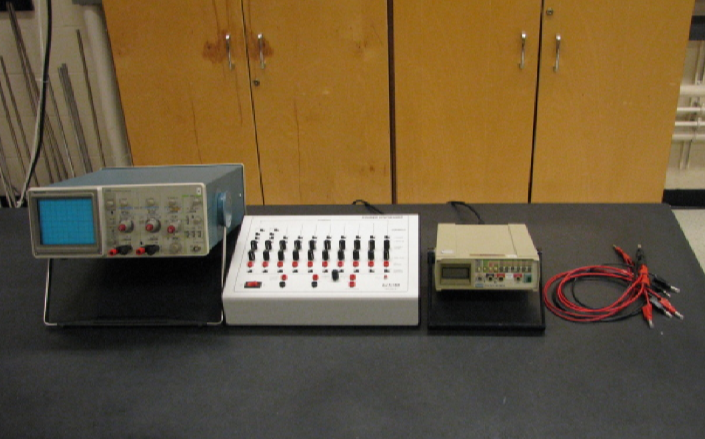
\includegraphics[scale = 0.8]{Images/FS1.PNG}
    \caption{Equipment used for Fourier series experiment}
    \label{fig:FS1}
\end{figure}

\section{Background}

All sounds are pressure waves transmitted through the aair. One method of describing these waves is to make use of a \Emph{Fourier series}. These series are composed of a multitude of sine and cosine functions of differing frequencies and amplitudes. Fourier series are used to deal with problems in such diverse fields as acoustics, geophysics, and astronomy. In 1747 D'Alembert formulated the general equation of a vibrating string. In 1753, Daniel Bernoulli formulated a solution of the vibrating string problem based on a series of sines and cosines. This started a debate whether smooth waves could be added up to produce waves with sharp jumps and corners. At first the smoothness problem seemed minor, but this same series began to appear elsewhere. In 1807, Fourier submitted a papaer that explained how to use this series to solve problems in heat transfer. This paper was critized, beacuse researchers did not accept that smooth waves could sum to jagged waves. Later analysts proved that a series sum of smooth functions could indeed produce a non-smooth result. Today, these series of sines and cosines are used routinely and are named \Emph{Fourier series} in honour of Jean-Baptiste Fourier.

\begin{figure}[H]
    \centering
    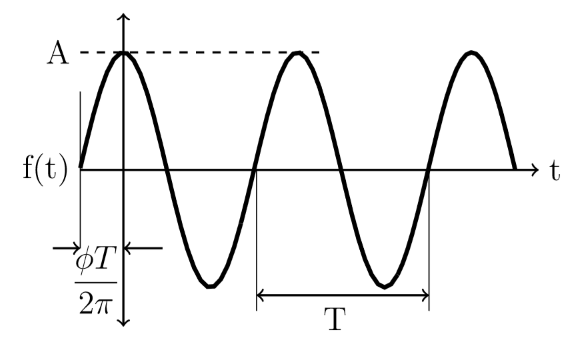
\includegraphics[scale = 0.8]{Images/FS2.PNG}
    \caption{Phase shifting of a sine wave.}
    \label{fig:FS2}
\end{figure}

Fourier series are based on the sine function. Sine is an example of a \Emph{periodic function}. It repeats at a regular interval called a \Emph{period}. As can be seen in Figure \ref{fig:FS2}, the period, $T$, is the length of time for one cycle of the wave. The frequency, $f = 1/T$, is the number of cycles in one second. A sine wave has two other parameters that can be varied. The \Emph{amplitude}, $A$, determines the height of the wave. The \Emph{phase shift}, $\phi$, is the amount the wave is shifted left or right. Sine waves are depicted mathematically by: \begin{equation}\ref{eq:FS1}
    f(t) = A\sin\left(\frac{2\pi}{T}t+\phi\right)
\end{equation}
The quantity $2\pi/T = 2\pi f = \omega$ is called the \Emph{angular frequency}.

\noindent Sine waves are added together to form Fourier series. In this light, the addition properties of two sine waves is a special case of Fourier series. If the frequency and the phase are identical, then the amplitude of the sum is the sum of the amplitudes. The frequency and phase remain unchanged. This means that \begin{equation}\label{eq:FS2}
    A\sin\left(\frac{2\pi}{T}t+\phi\right) + B\sin\left(\frac{2\pi}{T}t+\phi\right) = (A+B)\sin\left(\frac{2\pi}{T}t+\phi\right)
\end{equation}
The addition of sines with the same frequency but different phases introudces new properties. Suppose the two signals are separated by a phase of $\pi/2$. Then \begin{equation}\label{eq:FS3}
    A\sin\left(\frac{2\pi}{T}t\right) + B\sin\left(\frac{2\pi}{T}t+\frac{\pi}{2}\right) = C\sin\left(\frac{2\pi}{T}t+\phi\right)
\end{equation}
where \begin{equation}\label{eq:FS4}
    C = \sqrt{A^2+B^2}
\end{equation}
and \begin{equation}\label{eq:FS5}
    \phi = \tan^{-1}\left(\frac{B}{A}\right)
\end{equation}
The amplitude and phase of the sum are now functions of the amplitude and phase of the addends and are given by Equations \ref{eq:FS4} and \ref{eq:FS5}. However, the frequency remains unchanged and the sum is still a sinuosidal wave.

\noindent When sinusoidal waves of different frequencies are added, the sum is no longer a sine wave. For example, if sines of identical amplitude and unequal but close frequency are added, the result takes the form shown in Figure \ref{fig:FS3}. This is the phenomenon known as \Emph{beats}. A lower frequency envolope is seen to be riding on the outside of a higher frequency signal, known as a \Emph{carrier}, because it ``carries" the lower frequency beat signal along.

\begin{figure}[H]
    \centering
    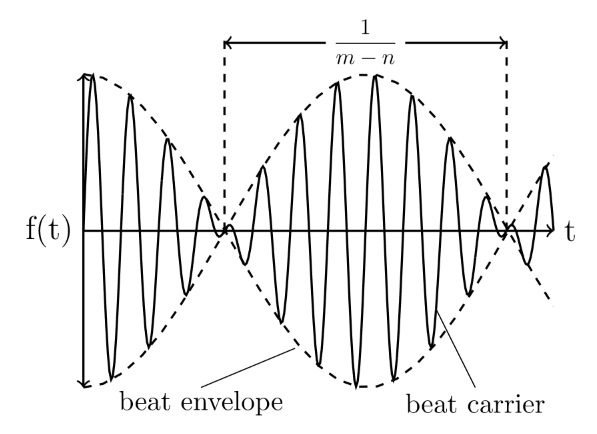
\includegraphics[scale = 0.8]{Images/FS3.PNG}
    \caption{An illustration of beat frequency}
    \label{fig:FS3}
\end{figure}

Mathematically, adding a sine wave of frequency $n$ to a sine wave of frequency $m$ yields the expression: \begin{equation}\label{eq:FS6}
    \sin(nx) + \sin(mx) = 2\sin\left[2\pi\left(\frac{m+n}{2}\right)x\right]\cos\left[2\pi\left(\frac{m-n}{2}\right)x\right]
\end{equation}
If $m$ and $n$ are close together, then Equation \ref{eq:FS6} can be though of as a time varying amplitude applied to a sine wave of frequency $(m+n)/2$. Although this time varying amplitude has frequency $(m-n)/2$, Figure \ref{fig:FS3} shows that the frequency at which the minimum value appears is twice this amount. So the beat envelope is head as the $m-n$.

\noindent The results of Equations \ref{eq:FS2} through \ref{eq:FS6} are found by use of standard trigonometric identities and results in waves that are repetitive in nature. However, the resulting sum of two sine waves need not repeat itself. An interesting fact about the addition of different frequencies, $m$ and $n$, is that the resulting wave is periodic only if there exists two rational numbers $p$ and $q$ such that \begin{equation}\label{eq:FS7}
    pm = qn
\end{equation}
i.e. if the numbers $m$ and $n$ are commensurable. If the frequencies $m$ and $n$ are commensurable, then the frequency of the sum is given by the \Emph{greatest common divisor} of $m$ and $n$.

\noindent A Fourier series generalizes the sum of two sine waves to the sum of an arbitrary number of sine and cosine waves. Each element of the series can havea difference amplitude. However, the frequency of any element must be an integer multiple of one frequency known as the \Emph{fundamental}. The integer multiples of the fundamental are known as \Emph{harmonics}. Suppose the fundamental has a period $T$. Then a Fourier series has the form \begin{equation}\label{eq:FS8}
    f(t) = a_0 + \sum_{n=1}^{\infty}\left(a_n\cos\left(\frac{2\pi n}{T}t\right) + b_n\sin\left(\frac{2\pi n}{T}t\right)\right)
\end{equation}
The constants $a_0,a_1,a_2,...,b_1,b_2,...$ are called \Emph{Fourier coefficients}. The most significant property of Fourier series is that any function, $f(t)$, that repeats with a period $T$ can be represented by such a series (assuming it doesn't have infinite discontinuities). This includes waves with sudden jumps and sharp corners.

\noindent A crucial problem is how to find the Fourier coefficients $a_0, a_n$ and $b_n$ for a given function $f(t)$, $n = 1,2,3,...$. The Fourier coefficients are calculated by the formulae \begin{equation}\label{eq:FS9}
    a_0 = \frac{1}{T}\int_0^Tf(t)dt
\end{equation}
\begin{equation}\label{eq:FS10}
    a_n = \frac{2}{T}\int_0^Tf(t)\cos\left(\frac{2\pi n}{T}r\right)dt 
\end{equation}
and \begin{equation}\label{eq:FS11}
    b_n = \frac{2}{T}\int_0^Tf(t)\sin\left(\frac{2\pi n}{T}r\right)dt 
\end{equation}
It can be seen from Equations \ref{eq:FS9}, \ref{eq:FS10}, and \ref{eq:FS11} that the Fourier coefficients for a function $f(t)$ are found by some form of integration over the period $T$. The reason for this is that certain integrals have the useful property of being zero for all terms of the Fourier series except one. They act as a filter that preserves one term of the Fourier series and eliminates all the others. In particular, we use the orthogonality relation for sine and cosine\begin{equation}\label{eq:FS12}
    \int_0^T\cos\left(\frac{2\pi n}{T}t\right)\sin\left(\frac{2\pi m}{T}t\right)dt = 0 \;\forall m,n \in \N
\end{equation}
\begin{equation}\label{eq:FS13}
    \int_0^T\cos\left(\frac{2\pi n}{T}t\right)\cos\left(\frac{2\pi m}{T}t\right)dt = \frac{L}{2}\delta_{mn}
\end{equation}
and \begin{equation}\label{eq:FS14}
    \int_0^T\sin\left(\frac{2\pi n}{T}t\right)\sin\left(\frac{2\pi m}{T}t\right)dt = \frac{L}{2}\delta_{mn}
\end{equation}


\begin{figure}[H]
    \centering
    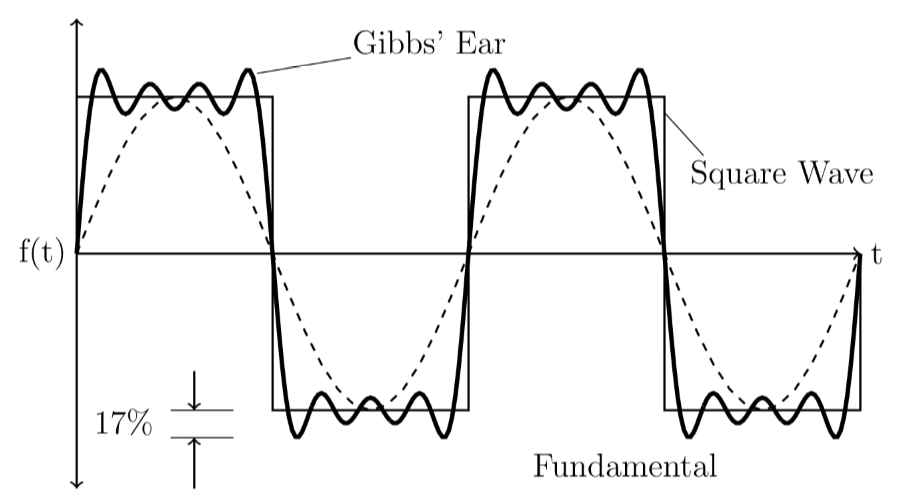
\includegraphics[scale = 0.8]{Images/FS4.PNG}
    \caption{An illustration of Gibbs' phenomenon.}
    \label{fig:FS4}
\end{figure}

\noindent In Figure \ref{fig:FS4} it can be seen that the shape is converging to a square wave. However, there seems to be a greater difficulty for the Fourier series to track at the discontinuity. There is a sudden jump or overshoot just before each rise and fall. This propensity for a Fourier series to overshoot at the edges is called \Emph{Gibbs' phenomenon} or \Emph{Gibbs Ears}. It turns out that this behaviour is a general property of all Fourier series. In fact, as more terms are added the ears get narrower, but their height may not decrease. For the square wave, it can be shown that the height of the ears nevr falls below $17\%$ above the square wave level.

\noindent This experiment examines the wave phenomena described here using an instrument called a \Emph{Fourier Synthesizer}. A Fourier synthesizer is an instrument that creates arbitrarily shaped periodic signals by use of Fourier series. The device generates two sine waves at a fundamental frequency of $440\;Hz$, as well as eight other harmonic sine waves at frequencies $880\;Hz, 1320\;Hz,...$ up to $3960\;Hz$. The phase and amplitude of each of these ten signals can be independently adjusted. Any combination of them can be added together. In this way the synthesizer can generate the first nine terms of any Fourier series.

\noindent The Fourier synthesizer used in this experiment is shown in Figure \ref{fig:FS5}. There are ten columns of controls. One column for each of the two fundamentals and eight harmonics. At the top of each column are the phase controls. Two switches select $90^{\circ}$ and $180^{\circ}$ phase shifts. The third phase control is continuously variable over a $90^{\circ}$ range. Together, these three controls provide a full $360^{\circ}$ phase adjustment range. Below the phase controls is an amplitude control to set the size of the signal. An in/out switch selects whether the column gets added to the output or not. Each column also includes an output point where the signal generated by that column can be measured.

\begin{figure}[H]
    \centering
    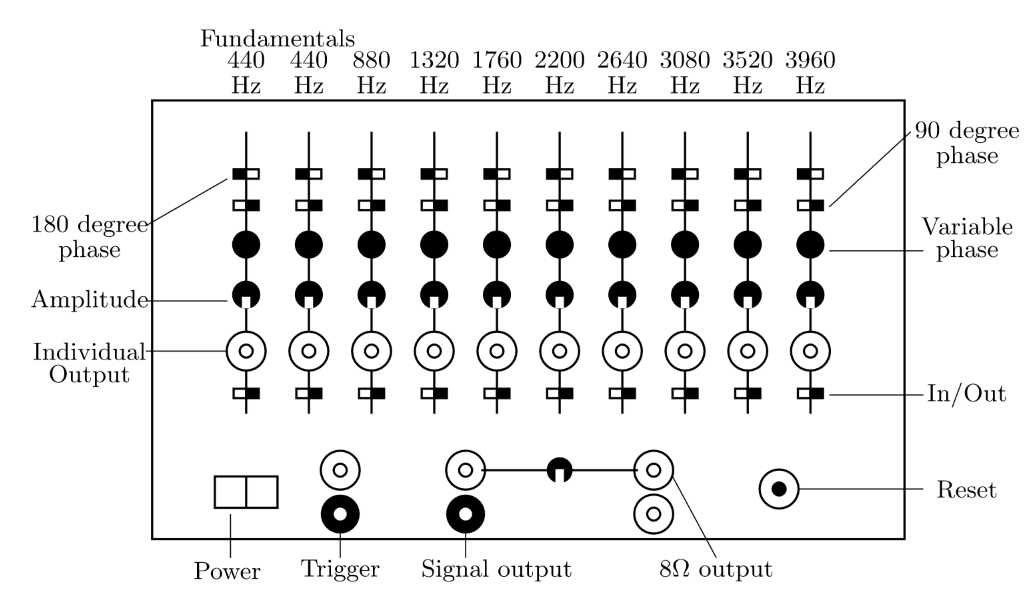
\includegraphics[scale = 0.8]{Images/FS5.PNG}
    \caption{A schematic picture of the Fourier synthesizer.}
    \label{fig:FS5}
\end{figure}

\noindent The third output is called a \Emph{trigger}. This signal is a square wave locked in phase with the fundamental. The edges of this square wave represent a phase angle of $0^{\circ}$. This signal serves as a time marker (metronome) against which phases can be measured. Lastly, the reset button is used to periodically resynchronize all the harmonics back together.

\noindent The synthesizer can be used to experimentally examine the properties of the addition of sine waves. Equation \ref{eq:FS3} can be examined by adding a sine wave to another phase shifted sine wave of the identical frequency. The amplitude and phase of the sum would be expected to vary in the systematic manner suggested by Equations \ref{eq:FS4} and \ref{eq:FS5}. Equation \ref{eq:FS6} and Figure \ref{fig:FS3} can be tested by observing the resulting waveform when sines of identical amplitude but differing frequency are added together. For best results, the chosen frequencies should be realtively close together. This suggests adding together high harmonics such as $5,6,7,8,$ and $9$. The resulting frequencies of the beat envelope and the beat carrier can be measured with an oscilloscope and compared against Equation \ref{eq:FS6}.

\noindent Similarly, Equation \ref{eq:FS7} can be examined by adding together two sinusoidal functions of arbitrary amplitude, phase, and frequency. The sum would be expected to have a frequency given by the greatest common divisor, independent of the amplitude and phase.

\noindent Most importantly, Equations \ref{eq:FS9}, \ref{eq:FS10}, and \ref{eq:FS11} can be used to find Fourier coefficients for various signals. It should be noted that the resulting shape is quite sensitive to the actual amplitude and phase of each harmonic. For best results, the amplitude of each harmonic should be set using the multimeter and the phase should be set using the oscilloscope.

\section{Experimental Procedure}


\begin{itemize}[leftmargin = 50pt]
    \item[Step 1:] Connect the Fourier synthesizer to the oscilloscope. One channel on the oscilloscope is best left connected to the trigger. The second channel on the oscilloscope is used to view the signal output or the individual output of each harmonic, whichever is most useful. The multimeter is connected to the individual output of whichever wave need to be measured at the time. A common ground should be used between all the equipment. For best results, the oscilloscope should be AC coupled.
    \item[Step 2:] To test Equation \ref{eq:FS3}, choose one fundamental to have an amplitude $A$ and the other amplitude $B$. Set the phase of $A$ to $0^{\circ}$ and the phase of $B$ to be $90^{\circ}$. The phase is set using the oscilloscope, by observing the alignment of the sine wave against one edge of the trigger. A phase shift of $90^{\circ}$ is $1/4$ of a period. Since the period is $1/440\;s$, the time shift for $90^{\circ}$ is $1/4\cdot440\;s \approx 570\;\mu s$. Fix the amplitude $A$ to some known value using the multimeter. Then, for at least eight different amplitudes of $B$, measure the amplitude of $C$ and the phase of the sum. Amplitude is best measured with the $AC$ voltmeter, and phase is best measured with the oscilloscope.
    \item[Step 3:] Choose any one of the following tests for the addition of sine waves of different frequency:
        \begin{enumerate}
            \item[(A)] Examine beats as given by Equation \ref{eq:FS6} and Figure \ref{fig:FS3}. Choose any two neighboring higher harmonics and set their amplitudes to be equal and the phases to be $0^{\circ}$. Measure the frequency of the beat envelope and beat carrier. Repeat for at least two other neighboring harmonics.
            \item[(B)] Examine the sum frequency predicted by Equation \ref{eq:FS7}. Choose any two frequencies with arbitrary non zero amplitudes and arbitrary phase. Measure the period of their sum. The sum frequency can be compared to the expected value given by the greatest common divisor of the individual frequencies. Repeat for at least two other combinations.
        \end{enumerate}
    \item[Step 4:] The synthesizer can generate a $9$ term Fourier series for the square wave, as seen in Figure \ref{fig:FS4}. A recipe for synthesizing the square is given in Table \ref{tab:FS1}. To synthesize a particular wave shape, each harmonic 1 through 9 must be set to a particular amplitude and phase. Each amplitude in the table is a percentage relative to a maximum amplitude within the first nine terms. Each phase angle is the number of degrees by which to shift that harmonic. Again, for best results, the AC voltmeter should be used to set the amplitude and the oscilloscope used to set the phase. 
        
        \begin{table}[H]
            \centering 
            \caption{Amplitudes and phase shifts required to synthesize a square wave.}
            \begin{tabular}{|c|c|c|c|c|c|c|c|c|c|}
                \hline
                $n$ & $1$ & $2$ & $3$ & $4$ & $5$ & $6$ & $7$ & $8$ & $9$ \\ \hline
                \% Ampl. & $100$ & $0.0 $& $33.3$ & $0.0$ & $20.0$ & $0.0$ & $14.3$ & $0.0$ & $11.1$ \\ 
                Phase & $90^{\circ}$ & $0^{\circ}$ & $90^{\circ}$ & $0^{\circ}$ & $90^{\circ}$ & $0^{\circ}$ & $90^{\circ}$ & $0^{\circ}$ & $90^{\circ}$ \\ \hline
            \end{tabular}
            \label{tab:FS1}
        \end{table}
    \item[Step 5:] Gibbs ears can be measured once the square wave has been synthesized. As each harmonic above number $1$ is ``switched in" record the height and width of Gibbs' ears. This data can be used to check whether the width steadily decreases, while the height goes no lower than $17\%$.
    \item[Step 6:] Synthesize one of the following waveforms. When synthesizing your signal do not trust the amplitude dials on the synthesizer. Instead set the amplitudes individually by measuring them with a multimeter.
        \begin{table}[H]
            \centering 
            \caption{Amplitudes and phase shifts required to synthesize a ramp.}
            \begin{tabular}{|c|c|c|c|c|c|c|c|c|c|}
                \hline
                $n$ & $1$ & $2$ & $3$ & $4$ & $5$ & $6$ & $7$ & $8$ & $9$ \\ \hline
                \% Ampl. & $100$ & $78.5 $& $11.1$ & $39.3$ & $4.0$ & $26.2$ & $2.0$ & $19.6$ & $1.2$ \\ 
                Phase & $0^{\circ}$ & $270^{\circ}$ & $0^{\circ}$ & $270^{\circ}$ & $0^{\circ}$ & $270^{\circ}$ & $0^{\circ}$ & $270^{\circ}$ & $0^{\circ}$ \\ \hline
            \end{tabular}
            \label{tab:FS2}
        \end{table}

        \begin{table}[H]
            \centering 
            \caption{Amplitudes and phase shifts required to synthesize a triangle.}
            \begin{tabular}{|c|c|c|c|c|c|c|c|c|c|}
                \hline
                $n$ & $1$ & $2$ & $3$ & $4$ & $5$ & $6$ & $7$ & $8$ & $9$ \\ \hline
                \% Ampl. & $100$ & $0.0 $& $11.1$ & $0.0$ & $4.0$ & $0.0$ & $2.0$ & $0.0$ & $1.2$ \\ 
                Phase & $0^{\circ}$ & $0^{\circ}$ & $0^{\circ}$ & $0^{\circ}$ & $0^{\circ}$ & $0^{\circ}$ & $0^{\circ}$ & $0^{\circ}$ & $0^{\circ}$ \\ \hline
            \end{tabular}
            \label{tab:FS3}
        \end{table}

        \begin{table}[H]
            \centering 
            \caption{Amplitudes and phase shifts required to synthesize a sawtooth.}
            \begin{tabular}{|c|c|c|c|c|c|c|c|c|c|}
                \hline
                $n$ & $1$ & $2$ & $3$ & $4$ & $5$ & $6$ & $7$ & $8$ & $9$ \\ \hline
                \% Ampl. & $100$ & $50 $& $33.3$ & $25.0$ & $20.0$ & $16.7$ & $14.3$ & $12.5$ & $11.1$ \\ 
                Phase & $90^{\circ}$ & $90^{\circ}$ & $90^{\circ}$ & $90^{\circ}$ & $90^{\circ}$ & $90^{\circ}$ & $90^{\circ}$ & $90^{\circ}$ & $90^{\circ}$ \\ \hline
            \end{tabular}
            \label{tab:FS4}
        \end{table}
    \item[Step 7:] Synthesize one of the following \Emph{rectified sine waves}.

        \begin{table}[H]
            \centering 
            \caption{Amplitudes and phase shifts required to synthesize a full rectified sine wave.}
            \begin{tabular}{|c|c|c|c|c|c|c|c|c|c|}
                \hline
                $n$ & $1$ & $2$ & $3$ & $4$ & $5$ & $6$ & $7$ & $8$ & $9$ \\ \hline
                \% Ampl. & $0$ & $100 $& $0$ & $20.0$ & $0.0$ & $8.6$ & $0$ & $4.8$ & $0$ \\ 
                Phase & $90^{\circ}$ & $0^{\circ}$ & $90^{\circ}$ & $0^{\circ}$ & $90^{\circ}$ & $0^{\circ}$ & $90^{\circ}$ & $0^{\circ}$ & $90^{\circ}$ \\ \hline
            \end{tabular}
            \label{tab:FS5}
        \end{table}
    \item[Step 8:] Three methods of transmitting binary signals (ones and zeros) are \Emph{frequency shift keying} (FSK), \Emph{amplitude shift keying} (ASK), and \Emph{phase shift keying}, as shown in Figures \ref{fig:FS6}, \ref{fig:FS7}, and \ref{fig:FS8}. If ASK is used, one cycle of a sine wave represents a one and a flat line is a zero. Likewise, FSK represents a one by one cycle of a sine wave and represents a zero by one cycle at a different frequency sine wave. For PSK, a one is designated by one cycle of a zero phase and a zero is one cycle of a $180^{\circ}$ phase shifted sine wave.

        \begin{figure}[H]
    \centering
    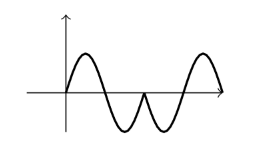
\includegraphics[scale = 0.8]{Images/FS6.PNG}
    \caption{Pulse shift keying}
    \label{fig:FS6}
\end{figure}

\begin{figure}[H]
    \centering
    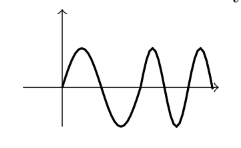
\includegraphics[scale = 0.8]{Images/FS7.PNG}
    \caption{Frequency shift keying}
    \label{fig:FS7}
\end{figure}

\begin{figure}[H]
    \centering
    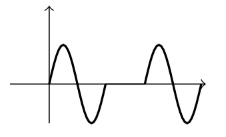
\includegraphics[scale = 0.8]{Images/FS8.PNG}
    \caption{Amplitude shift keying}
    \label{fig:FS8}
\end{figure}

        \begin{table}[H]
            \centering 
            \caption{Amplitudes and phase shifts required for PSK.}
            \begin{tabular}{|c|c|c|c|c|c|c|c|c|c|}
                \hline
                $n$ & $1$ & $2$ & $3$ & $4$ & $5$ & $6$ & $7$ & $8$ & $9$ \\ \hline
                \% Ampl. & $100$ & $0.0 $& $60.0$ & $0.0$ & $14.3$ & $0.0$ & $6.7$ & $0.0$ & $3.9$ \\ 
                Phase & $0^{\circ}$ & $0^{\circ}$ & $180^{\circ}$ & $0^{\circ}$ & $180^{\circ}$ & $0^{\circ}$ & $180^{\circ}$ & $0^{\circ}$ & $180^{\circ}$ \\ \hline
            \end{tabular}
            \label{tab:FS6}
        \end{table}

        \begin{table}[H]
            \centering 
            \caption{Amplitudes and phase shifts required for FSK.}
            \begin{tabular}{|c|c|c|c|c|c|c|c|c|c|}
                \hline
                $n$ & $1$ & $2$ & $3$ & $4$ & $5$ & $6$ & $7$ & $8$ & $9$ \\ \hline
                \% Ampl. & $56.8$ & $100.0 $& $41.6$ & $22.0$ & $8.4$ & $0.0$ & $2.9$ & $2.1$ & $0.0$ \\ 
                Phase & $30^{\circ}$ & $150^{\circ}$ & $90^{\circ}$ & $30^{\circ}$ & $330^{\circ}$ & $0^{\circ}$ & $30^{\circ}$ & $330^{\circ}$ & $0^{\circ}$ \\ \hline
            \end{tabular}
            \label{tab:FS7}
        \end{table}

        \begin{table}[H]
            \centering 
            \caption{Amplitudes and phase shifts required for ASK.}
            \begin{tabular}{|c|c|c|c|c|c|c|c|c|c|}
                \hline
                $n$ & $1$ & $2$ & $3$ & $4$ & $5$ & $6$ & $7$ & $8$ & $9$ \\ \hline
                \% Ampl. & $84.9$ & $100.0 $& $50.9$ & $0.0$ & $12.1$ & $0.0$ & $5.7$ & $0.0$ & $3.3$ \\ 
                Phase & $0^{\circ}$ & $90^{\circ}$ & $180^{\circ}$ & $0^{\circ}$ & $180^{\circ}$ & $0^{\circ}$ & $180^{\circ}$ & $0^{\circ}$ & $180^{\circ}$ \\ \hline
            \end{tabular}
            \label{tab:FS8}
        \end{table}
\end{itemize}

\section{Error Analysis}

Generally, the errors in an experiment arise from \Emph{systematic errors} in the apparatus and \Emph{measurement errors} in the instruments. In this experiment, the measurement erros are determined by the accuracy of the osciloscope and the multimeter. The systematic errors arise from the behaviour and performance of the Fourier synthesizer. The measurement errors of the oscilloscope and multimeter can be readily estimated.

However, there are many possible sources of systematic error lurking inside the synthesizer. The fundamental and harmonic sine waves generated by the synthesizer have some \Emph{distortion}. Also, the summation of all the components is not mathematically perfect. Furthermore, the synchronization of the hermonics to each other and to the fundamental is not exact. The magnitude of these and other internal errors is essentially unknown. 



%%%%%%%%%%%%%%%%%%%%%% Chapter 1.9
\chapter{AC Circuit and RLC Resonance}


\begin{figure}[H]
    \centering
    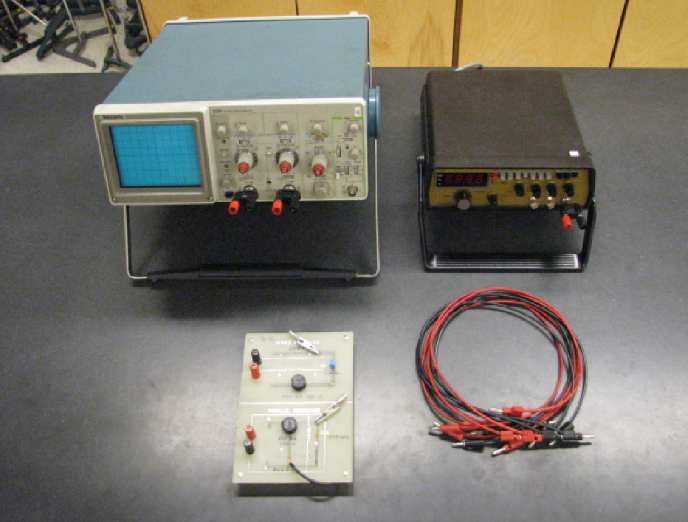
\includegraphics[scale = 0.8]{Images/Res1.PNG}
    \caption{Equipment used to investigate a resonance in RLC circuits.}
    \label{fig:Res1}
\end{figure}


\section{Background}


The current delivered to homes and factories is an oscillating function of time. This is called \Emph{alternating current}, of \Emph{AC}. All the appliances connected to ordinary outlets in homes therefore involve circuits with oscillating currents. Furthermore, electronic devices, such as radio transmitters and receivers, involve a variety of circuits with oscillating currents of high frequency. Many of these circuits have natural frequencies of oscillation. Such circuits exhibit the phenomenon of \Emph{reconance} when the natural frequency matches the frequency of a signal applied to the circuit. For instance, the tuning of a radio relies on an oscillating circuit whose frequency of oscillation is adjusted by means of a variable capacitor so that it matches the frequency of the radio signal.

\noindent A common circuit known as the \Emph{RLC circuit} exhibits the phenomenon of resonance. It is named RLC becuase it includes a resistor, a capacitor, and an inductor. In this laboratory we will only analyse a series RLC circuit.

\subsection{Series RLC Circuits}

The series RLC circuit used in this experiment is shown in Figure \ref{fig:Res2}. The values of resistance, $R_r$, capacitance, $C$, and inductance, $L$, are written on the components themselves. The total resistance of the circuit, $R$, is the sum of the resistance of the resistor, $R_r$, and the inductor (solenoid), $R_L$.

\begin{figure}[H]
    \centering
    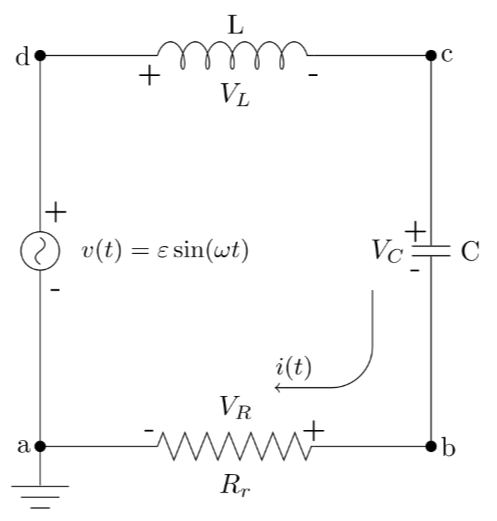
\includegraphics[scale = 0.8]{Images/Res2.PNG}
    \caption{Series RLC circuit.}
    \label{fig:Res2}
\end{figure}

Assume that the internal resistance of the function generator can be ignored and choose the input signal to be $v(t) = \varepsilon\sin(\omega t)$, where $\varepsilon$ is the maximum emf. The emf acts as a driving force that moves the charge in the circuit. An application of \Emph{Kirchhoff's voltage law} gives \begin{equation}\label{eq:Res1}
    \sum V = 0 = V_L + V_C + V_R - \varepsilon\sin(\omega t)
\end{equation}
where \begin{equation}\label{eq:Res2}
    V_C = \frac{1}{C}\int i\cdot dt 
\end{equation}
\begin{equation}\label{eq:Res3}
    V_L = L\frac{di}{dt}
\end{equation}
and \begin{equation}\label{eq:Res4}
    V_R = iR
\end{equation}
are the AC voltages across each component.

\noindent Substituting Equations \ref{eq:Res2}, \ref{eq:Res3}, and \ref{eq:Res4} into Equation \ref{eq:Res1} and rearranging gives the expression \begin{equation}\label{eq:Res5}
    \varepsilon\sin(\omega t) = \frac{1}{C}\int i\cdot dt + L\frac{di}{dt} + iR
\end{equation}
Differentiating both sides with respect to time, $t$, to remove the integral, yields the differential equation \begin{equation}\label{eq:Res6}
    \varepsilon\omega\cos(\omega t) = \frac{i}{C} + L\frac{d^2i}{dt^2} + R\frac{di}{dt}
\end{equation}
The steady state solution of this equation is \begin{equation}\label{eq:Res7}
    i(t) = \frac{\varepsilon}{\sqrt{R^2+\left(\omega L - \frac{1}{\omega C}\right)^2}}\cdot\sin(\omega t - \phi)
\end{equation}
where \begin{equation}\label{eq:Res8}
    \phi = \tan^{-1}\left[\frac{1}{R}\left(\omega L - \frac{1}{\omega C}\right)\right]
\end{equation}
The same equation can be obtained through the analysis of the circuit's complex impedance.

\noindent The \Emph{angular frequency}, $\omega$, is $2\pi f$, where $f$ is the frequency in cycles per second, or Hertz (Hz). Equations \ref{eq:Res7} and \ref{eq:Res8} imply that the current flowing in a series RLC circuit is a sine wave with an amplitude that changes with frequency and a phase difference from the signal generator that also changes with frequency. So the behaviour of the circuit strongly depends on the frequency of the applied voltage.

\noindent For Equation \ref{eq:Res7}, the current, $i(t)$, becomes an extremum when $\omega^2 = 1/LC$. The condition when the amplitude of $i(t)$ is an extremum is known as \Emph{amplitude resonance}. For series RLC circuits, the extremum turns out to be a \Emph{maximum}. Thus, at amplitude resonance the current flowing in the circuit has maximum amplitude. At all other frequencies, the current flowing in the circuit is smaller. This property makes the series RLC circuit useful in filters where a response at one frequency is preferred over all other frequencies. This is what happens in radio receivers when one station is selected. The frequency corresponding to the carrier of that station is chosen to be the amplitude resonant frequency.

\noindent When $\omega^2 = 1/LC$, Equation \ref{eq:Res8} implies that $\phi = 0$. The condition when $\phi = 0$ is called \Emph{phase resonance}. At phase resonance, the signals at points $d$ and $b$ in Figure \ref{fig:Res2} are in phase. So there is no phase difference between the applied voltage and the current through the circuit. In series RLC circuits, amplitude and phase resonance both happen at the \Emph{same frequency}. In other types of circuits this is not necessarily true.

\noindent The oscilloscope screen in Figure \ref{fig:Res3} shows two signals that are not in phase with each other. A phase difference between two waveforms is usually reported as an angle. Since horizontal distances on an oscilloscope are in terms of time, a conversion from time to angle has to be made. This is done by noting that the time for a full cycle is $2\pi$ rad, so the actual phase difference as an angle is found by determining it as a fraction of one cycle, and multiplying by $2\pi$ rad.

\begin{figure}[H]
    \centering
    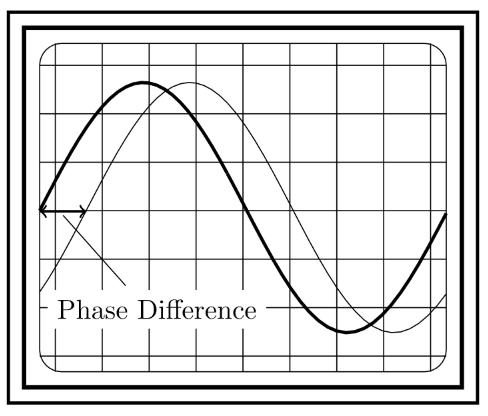
\includegraphics[scale = 0.8]{Images/Res3.PNG}
    \caption{An illustration of phase difference}
    \label{fig:Res3}
\end{figure}

To measure a phase difference between two sine waves necessarily implies that they have the same frequency. The phase difference between two sine waves of various frequencies is not constant. Also, notice that the two sinusoidal waveforms depicted in Figure \ref{fig:Res3} have the same amplitude allowing for accurate measurement of the phase difference. Since in general, it is unlikely that any two signals have the same amplitude, a special control is available on the oscilloscope to shift amplitudes without requiring a change to the input signal. This control is called the \Emph{vertical calibration} adjustment. To make two signals have the same displayed amplitude simply modify the vertical calibration of one channel. After the phase measurement is completed, remember to return the vertical claibration setting back to normal, otherwise further vertical measurements will be incorrect.

\noindent When $i(t)$ becomes an extremum, the input frequency matches the \Emph{natural frequency} of the circuit. This is manifested as a voltage extremum on the oscilloscope screen. Thus, when searching for frequencies at which $i(t)$ becomes an extremum, look for frequencies corresponding to a voltage extremum on the oscilloscope screen. The reason for voltage measurements rather than current measurements is due to the fact that the oscilloscope only displays voltages. Moreover, the signal at point $b$ is the voltage across the resistor, which is directly proportional to the current by Ohm's law.

\section{Experimental Procedure}

\begin{itemize}[leftmargin = 50pt]
    \item[Step 1:] Inspect the function generator and the dual channel oscilloscope. Make sure that the function generator is set to a sine wave output. Also, set the scope to show both channels on the screen simultaneously as this will be needed to verify the phase resonance of the circuits.
    \item[Step 2:] For the \Emph{series RLC circuit}, setup the experiment as in Figure \ref{fig:Res4}. Connect both the function generator and channel 1 of the oscilloscope between $d$ and $a$, the input pins. Thus the trace on channel 1 will represent the input signal from the function generator. Connect channel 2 of the oscilloscope between $b$ and $a$. The channel 2 trace will then be directly proportional to the current going through the circuit.

        \begin{figure}[H]
    \centering
    \includegraphics[scale = 0.8]{Images/Res4.PNG}
    \caption{Series RLC circuit setup.}
    \label{fig:Res4}
\end{figure}
    \item[Step 3:] Find the amplitude/phase resonance by scanning through frequencies near the theoretical value. Stop varying the frequency when the channel 2 trace has its amplitude extremum. Record the experimental resonant frequency from the function generator. Verify that the frequency for the amplitude resonance is the same as the frequency for phase resonance $(\phi = 0)$.
    \item[Step 4:] For the resonant frequency and at least 50 other frequencies, some below and some above the resonant frequency, record the peak-to-peak voltage value from the oscilloscope. Select your frequencies so you can precisely determine the maximum value and be able to observe the out-of-resonance behaviour of the circuit.
\end{itemize}

\section{Error Analysis}

The internal resistance of the function generator is ignored in this experiment. Consider all values written on the circuit boards as exact. The error in an oscilloscope measurement is half the resolution of the measurement scale. Remember to make detailed notes on which voltage scale and time scale the oscilloscope is set on when recording data.

\noindent There are two errors associated with the function generator frequency. A \Emph{drift error} caused by temperature variations inside the function generator and a \Emph{quantization error} which is associated with any digital instrument. The drift error can be estimated by oscerving varitions in the output frequency. While you are making measurements, take not of the maximum and minimum frequency values displayed on the function generator. The difference between them divided by two gives the associated drift error. If the function generator has been on for some time then no drift in frequency values may be observable. In this case, the only error associated with the frequency will be the quantization error.

\noindent The rror resulting from conversion of a frequency to a digital display is called the quantization error. Manufacturers usually give the value of this error as plus or minus one number in the smallest digit of the display. The manual accompanying the B and K Precision Function Generator lists this value as $\pm 1$ count.

\noindent Take the error in frequency to be the sum of the drift and quantization errors. 





%%%%%%%%%%%%%%%%%%%%%% Chapter 1.10
\chapter{AC Circuits and Voltage Dividers}

\section{Resistor-Capacitor Filters}

There are two possible RC configurations, one with the output voltage taken over the resistor, and the other with the output taken across the capacitor. If the output is taken across the capacitor, we obtain a low pass filter, and if the output is taken across the resistor, we obtain a high pass filter.

\begin{defn}
    The frequency at which the magnitude of the ratio of output voltage to input voltage is $10^{-3/20}\approx 0.7079$ is called the \Emph{cutoff frequency}. This is the frequency at which half the input power is transferred to the output and is therefore sometimes called the $-3\;dB$ frequency.
\end{defn}

The cutoff frequency of a filter is considered to be the frequency at which the filter begins to block or attenuate the input signal.

\begin{defn}
    An \Emph{all-pass filter} requires two resistor-capacitor pairs whose products, ($RC$), are equal. This configuration provides a constant ratio of $V_{out}$ to $V_{in}$ at all frequencies by rendering stray capacitance and inductance insignificant.
\end{defn}

\begin{defn}
    The \Emph{gain function} $G(\omega)$ is the transfer function of any circuit. It is the ratio of $V_{out}$ to $V_{in}$ (phase and amplitude count) as a function of frequency.
\end{defn}

\section{Attenuator Probe Adjustments and Compensations}

Since many measurements (high-impedance and high-frequency) require an attenuator probe, you should make sure it is compensated as a routine part of turning on the scope. A square wave intended for probe calibration and compensation is always available on the scope's front panel. Probe compensation is adjustable via a screwdriver slot on the probe body or connector. The display of an undistorted square wave is a quick indication of correct compensation.

If we adjust the probe capacitor $C_p$ to the correct value, a compensating amount of high frequency information will be bypassed around the probe resistor, and a square wave will have both flat tops and bottoms. We see spikes for too much high-frequency response from the probe, and curved edges for too little high frequency response.

\begin{rmk}
    In the context of high-frequency measurements, the total input impedance drops as the frequency increases because stray capacitance is in parallel to the probe. This is unavoidable and makes the $\times 10$ probe even more important in high-frequency environments to minimize loading errors.
\end{rmk}



%%%%%%%%%%%%%%%%%%%%%% Chapter 1.11
\chapter{AC Circuits, Waveforms, and Phase}

\section{Measurement of Sine Wave Amplitudes}

Digital multimeters (DMMs) are more convenient and accurate for measuring DC voltages, currents, and sinusoidal AC voltages and currents than oscilloscopes.

We can specify the amplitude of a sine wave in four ways: using the peak-to-peak value, the peak value, the average value, and the root mean square (RMS) value. The peak value is the value at the top of the waveform, the peak-to-peak is twice the peak, or the difference between the maximum and minimum. The RMS value is found by taking the square root of the average of the squared values of the current. This value of the sine wave current will produce the same heating effect in a resistor as a DC current of the same magnitude, since the power dissipated by a resistor is proportional to the square of the current running through it ($P = I^2R$).

The DMM measures the RMS voltage. The oscilloscope can be best used to measure the peak-to-peak voltage.

\section{RC Circuit Current and Voltage Relationships}

\begin{rmk}
    \Emph{Dual trace observation}: If there are two input signals, one to CH1 and one to CH2, you can only trigger on one signal or the other. To operate the oscilloscope such that you can observe two signals simultaneously you must select the vertical axis mode button [DUAL] and select either ALT or CHOP.
\end{rmk}

\begin{rmk}
    \Emph{Measuring phase difference}: Phase difference can be measured by the distance of separation between the signals when crossing the zero line. This time, divided by the time duration of one full cycle, defines the fraction of a cycle of phase difference. We know $1$ cycle $= 2\pi$, so the fraction must be multiplied by the appropriate factor to be expressed in radians.
\end{rmk}


%%%%%%%%%%%%%%%%%%%%%% Chapter 1.12
\chapter{Inductor-Resistor-Capacitor Filters}

\section{Quality Factor}

The quality factor of an oscillator, $Q$, is a dimensionless parameter describing how slowly oscillations decay. More specifically, it roughly measures the number of oscillations (i.e. up to a constant) before the energy of the oscillator at a given time would decrease by a factor of $e$ in the absence of a driving mechanism. 

In the parallel resonant circuit, the $Q$ value is directly proportional to the resistance. With a relatively large resistance, the circuit will be \Emph{underdamped}. This is chracterized by exponentially decaying sinusoidal electrical oscillations in response to an impulse. \Emph{Critical damping} occurs with a slightly smaller resistance and is the point at which the circuit no longer oscillates, but returns in the minimum possible time to zero output after the impulse. \Emph{Overdamping} occurs with a small resistance, and is evidenced by capacitor charge returning more slowly than the case of critical damping.

When a parallel LRC circuit is used as a filter, the $Q$ factor determines the bandwidth of the filter's response in frequency space. With a $Q$ of $2$ or $3$, the response begins to be noticeably peaked. When $Q$ is larger than $10$, the filter's amplitude response is peaked by more than an order of magnitude at resonance. All measurements are traditionally normalized to the peak amplitude and to the frequency at which that peak occurs.

\subsection{Important formulas}

The impedance of an LRC circuit, with the components connected in parallel is \begin{equation*}
    \frac{1}{Z_{LRC}} = \frac{1}{R}  + \frac{1}{j\omega L} + j\omega C
\end{equation*}
and resonance frequency, $f_0$, is given by \begin{equation*}
    f_0 = \frac{1}{2\pi \sqrt{LC}}
\end{equation*}
the quality factor is \begin{equation*}
    Q = \frac{f_0}{Bandwidth} = RC\omega_0
\end{equation*}
and the bandwidth is \begin{equation*}
    Bandwidth = f_{high3dB} - f_{low3dB} = \frac{1}{2\pi RC}
\end{equation*}



%%%%%%%%%%%%%%%%%%%%%% Chapter 1.13
\chapter{Transformer Voltage Gain, Ground Isolation}

%%%%%%%%%%%%%%%%%%%%%% Chapter 1.14
\chapter{Intro to Operational Amplifiers}

%%%%%%%%%%%%%%%%%%%%%% Chapter 1.15
\chapter{Inductor-Resistor-Capacitor Filters}


%%%%%%%%%%%%%%%%%%%%%% Chapter 1.16
\chapter{Bandwidth and Stability}

\section{Lecture Notes}

Note that an ideal op-amp is a perfect linear differential operator. Additionally recall that $V_{out} = A(V_+-V_-)$ at all frequencies. But if the open loop gain $A$ is infinite always, as $\omega\rightarrow \infty$ we have $\frac{dV_{out}}{dt}\rightarrow \infty$. If there is any capacitance $q = CV$, $I\rightarrow \infty$ which is unphysical!

For any real op=amp we have $A = A(\omega)$ with $\lim\limits_{\omega\rightarrow \infty}A(\omega) = 0$. We take a low pass filter on the gain: the open loop gain $A(\omega)$ is deliberately shaped as $1/$ in the intended operating range.

In a log-log scale we have the following plot:

\begin{figure}[H]
    \centering
    \begin{tikzpicture}[x=0.75pt,y=0.75pt,yscale=-1,xscale=1]
%uncomment if require: \path (0,300); %set diagram left start at 0, and has height of 300

%Shape: Axis 2D [id:dp5423974030492535] 
\draw  (50,218.65) -- (298.67,218.65)(74.87,73) -- (74.87,234.83) (291.67,213.65) -- (298.67,218.65) -- (291.67,223.65) (69.87,80) -- (74.87,73) -- (79.87,80)  ;
%Curve Lines [id:da03190911322917622] 
\draw    (75.67,90.83) .. controls (183.67,91.83) and (169.67,97.83) .. (240.67,210.83) ;
%Straight Lines [id:da8786320512830679] 
\draw  [dash pattern={on 4.5pt off 4.5pt}]  (74.67,182.83) -- (280.67,183.83) ;
%Straight Lines [id:da9841736453899332] 
\draw  [dash pattern={on 4.5pt off 4.5pt}]  (224.67,70.83) -- (224.67,218.83) ;

% Text Node
\draw (305,211.4) node [anchor=north west][inner sep=0.75pt]    {$f$};
% Text Node
\draw (33,142.4) node [anchor=north west][inner sep=0.75pt]    {$A( \omega )$};
% Text Node
\draw (45,77.4) node [anchor=north west][inner sep=0.75pt]    {$A_{0}$};
% Text Node
\draw (207,232.4) node [anchor=north west][inner sep=0.75pt]    {$GBWP$};
% Text Node
\draw (60,173.4) node [anchor=north west][inner sep=0.75pt]    {$1$};


\end{tikzpicture}
    \caption{Open loop gain as a function of $f$ in a log-log  scale}
    \label{fig:GBWP}
\end{figure}

The slope of the linear portion on this figure is $1/f$. The \Emph{Gain Bandwidth Product} (GBWP) is the frequency at which the gain $A(\omega)$ is equal to 1. We hope to express these ideas using some well known equations.

We consider the following op amp:

Recall $V_{out} = A(V_+ - V_-)$. We define $\beta = \frac{1}{Gain} = \frac{R_1}{R_1+R_f}$. Then $V_{out} = A(V_{in}-\beta V_{out}) = AV_{in} - A\beta V_{out})$, so $V_{out}(1+A\beta) = AV_{in}$. so our closed loop gain is \begin{equation*}
    \frac{V_{out}}{V_{in}} = \frac{A}{1+A\beta}
\end{equation*}



\begin{note}
    Not all op amps preserve the phase at the output. We need the negative feedback to be going back to the inverting input, or otherwise the devices will begin to oscillate.
\end{note}


\subsection{Frequency Rolloff}

The \Emph{frequency roll off} is generally $-20\;dB/$decade. In other words, the gain is down by a factor of $10$ for every $10\times$ increase in frequency. \begin{equation*}
    -20\;dB = 20\log\left(\frac{V_{out}}{V_{in}}\right) \implies \frac{V_{out}}{V_{in}} = \frac{1}{10}
\end{equation*}
Equivalently this is $-6\;dB/$octave, where an octave is a halving/doubling in frequency, so $\frac{V_{out}}{V_{in}} = 10^{-3/10}$.




%%%%%%%%%%%%%%%%%%%%%% Chapter 1.17
\chapter{Basic OpAmp Difference Amplifier}

\section{Lecture Notes: Common Mode Refection}

We consider a \Emph{difference amplifier}.

\begin{figure}[H]
    \centering
    \begin{tikzpicture}[x=0.75pt,y=0.75pt,yscale=-1,xscale=1]
%uncomment if require: \path (0,300); %set diagram left start at 0, and has height of 300

%Shape: Triangle [id:dp9349243300744214] 
\draw   (266.56,135) -- (204.56,181.67) -- (204.56,88.33) -- cycle ;
%Straight Lines [id:da9016223177337594] 
\draw    (204.78,115.22) -- (161.39,115.17) ;
%Straight Lines [id:da19593682684243774] 
\draw    (179.56,226) -- (179.53,235.33) ;
%Straight Lines [id:da06399294948266676] 
\draw    (166.78,235.33) -- (192.28,235.33) ;
%Straight Lines [id:da8704020961222847] 
\draw    (172.45,240.33) -- (187,240.33) ;
%Straight Lines [id:da3636303635539251] 
\draw    (175.67,245.33) -- (183.67,245.33) ;
%Shape: Resistor [id:dp5587621278879087] 
\draw   (182.78,56.56) -- (194.36,56.56) -- (196.93,44.22) -- (202.08,68.89) -- (207.22,44.22) -- (212.37,68.89) -- (217.52,44.22) -- (222.66,68.89) -- (227.81,44.22) -- (232.96,68.89) -- (235.53,56.56) -- (247.11,56.56) ;
%Shape: Resistor [id:dp15339117302166838] 
\draw   (97.06,115.17) -- (108.64,115.17) -- (111.21,102.83) -- (116.36,127.5) -- (121.5,102.83) -- (126.65,127.5) -- (131.8,102.83) -- (136.94,127.5) -- (142.09,102.83) -- (147.24,127.5) -- (149.81,115.17) -- (161.39,115.17) ;
%Straight Lines [id:da06424554821135597] 
\draw    (182.78,56.56) -- (183.08,115.19) ;
%Straight Lines [id:da2914585460309578] 
\draw    (247.11,56.56) -- (304.78,56.56) ;
%Straight Lines [id:da3363888323999258] 
\draw    (330.44,133.62) -- (266.13,134.72) ;
%Shape: Circle [id:dp9521602314204742] 
\draw   (344.88,133.38) .. controls (344.95,137.37) and (341.77,140.66) .. (337.78,140.72) .. controls (333.79,140.79) and (330.51,137.61) .. (330.44,133.62) .. controls (330.37,129.63) and (333.55,126.35) .. (337.54,126.28) .. controls (341.53,126.21) and (344.82,129.39) .. (344.88,133.38) -- cycle ;
%Straight Lines [id:da12185081603205372] 
\draw    (304.78,56.56) -- (305.44,133.89) ;
%Shape: Circle [id:dp9989873427873128] 
\draw   (82.61,115.17) .. controls (82.61,111.18) and (85.84,107.94) .. (89.83,107.94) .. controls (93.82,107.94) and (97.06,111.18) .. (97.06,115.17) .. controls (97.06,119.16) and (93.82,122.39) .. (89.83,122.39) .. controls (85.84,122.39) and (82.61,119.16) .. (82.61,115.17) -- cycle ;
%Straight Lines [id:da51088313252288] 
\draw    (204.28,161.72) -- (160.89,161.67) ;
%Shape: Resistor [id:dp982608519362788] 
\draw   (96.56,161.67) -- (108.14,161.67) -- (110.71,149.33) -- (115.86,174) -- (121,149.33) -- (126.15,174) -- (131.3,149.33) -- (136.44,174) -- (141.59,149.33) -- (146.74,174) -- (149.31,161.67) -- (160.89,161.67) ;
%Shape: Circle [id:dp2678251554408111] 
\draw   (82.11,161.67) .. controls (82.11,157.68) and (85.34,154.44) .. (89.33,154.44) .. controls (93.32,154.44) and (96.56,157.68) .. (96.56,161.67) .. controls (96.56,165.66) and (93.32,168.89) .. (89.33,168.89) .. controls (85.34,168.89) and (82.11,165.66) .. (82.11,161.67) -- cycle ;
%Shape: Resistor [id:dp570733345623794] 
\draw   (179.72,162) -- (179.72,173.58) -- (192.06,176.15) -- (167.39,181.3) -- (192.06,186.45) -- (167.39,191.59) -- (192.06,196.74) -- (167.39,201.89) -- (192.06,207.03) -- (167.39,212.18) -- (179.72,214.75) -- (179.72,226.33) ;

% Text Node
\draw (206.89,151.4) node [anchor=north west][inner sep=0.75pt]    {$+$};
% Text Node
\draw (207.56,105.73) node [anchor=north west][inner sep=0.75pt]    {$-$};
% Text Node
\draw (57,152.4) node [anchor=north west][inner sep=0.75pt]    {$V_{2}$};
% Text Node
\draw (58,105.4) node [anchor=north west][inner sep=0.75pt]    {$V_{1}$};
% Text Node
\draw (347.33,124.18) node [anchor=north west][inner sep=0.75pt]    {$V_{out}$};
% Text Node
\draw (194.06,189.85) node [anchor=north west][inner sep=0.75pt]    {$R_{f}$};
% Text Node
\draw (117.86,177.4) node [anchor=north west][inner sep=0.75pt]    {$R_{in}$};
% Text Node
\draw (113.86,84.07) node [anchor=north west][inner sep=0.75pt]    {$R_{in}$};
% Text Node
\draw (200.72,23.18) node [anchor=north west][inner sep=0.75pt]    {$R_{f}$};


\end{tikzpicture}
    \caption{Difference Amplifier}
    \label{fig:DiffAmp}
\end{figure}

We have the expression \begin{equation*}
    V_{out} = \frac{R_f}{R_{in}}\left(V_2-V_1\right)
\end{equation*}
Note for this to work we need to assume that our $R_{in}$'s and $R_f$'s are identical. Here the output is proportional to the difference in the two signal.

Now, the \Emph{Common Mode Rejection Ratio} (CMRR). In general we have $\frac{\text{Gain diff amp}}{\text{Gain common mode}} \sim 500$ to $50000$. The gain of the diff amplifier is $\frac{V_{out}}{V_2-V_1}$, while the common mode gain is $\frac{V'_{out}}{V_{in}}$ where here $V_2 = V_1 = V_{in}$. Both inputs have the same signal.


%%%%%%%%%%%%%%%%%%%%%% Chapter 1.18
\chapter{Operational Amplifier Comparator}


%%%%%%%%%%%%%%%%%%%%%% Chapter 1.19
\chapter{Active Filters and Anti-Aliasing Filters}

\section{Lecture Notes: Sampling, Aliasing, and Analog Filters}

\begin{qst}
    How can we accurately generate a set of discrete samples?
\end{qst}
Recall the Nyquist theorem: to generate an unambiguous representation of a waveform at $\frac{1}{2}$ the sampling frequency we must limit the maximum frequency in the signal to NO GREATER than $\frac{1}{2}$ the sampling frequency. 

We must avoid aliasing - where we have one frequency masquerading as another! 

\subsection{Filters}

\begin{qst}
    How can we keep our maximum frequency within a safe frequency range?
\end{qst}

When building a circuit we want about about a quarter of the Nyquist frequency gap between our frequencies after filtering and the Nyquist frequency. This is to ensure no frequencies appear above the Nyquist, $f_N$. A simple filter with a $\frac{1}{f}$ rolloff is not sufficient. We must construct a circuit of cascading filters to give a stronger rolloff.





%%%%%%%%%%%%%%%%%%%%%% Chapter 1.20 
\chapter{Swept Frequency Waveform Generator, DFT}


Many laboratory function generators have the capability of changing frequency according to a voltage input. Most include an internal ramp generator to be used to smoothly tune the function generator across a known range of frequencies. THis allows the automation of some otherwise tedious measurements. 

Used alone, the swept frequency generator can simplify/automate the task of plotting the frequency response of filters. The oscilloscope can then be used to present an $X-Y$ plot of a simple $RC$ or $LRC$ filter's frequency response.

The Fourier Spectrum Scanner is an addition to the frequency generator. For the Fourier Spectrum Scanner, a multiplier is used in the ``time domain" to produce sums and differences in the ``frequency domain." If we follow the multiplier with a low-pass filter, we are able to plot only the difference frequency. This can produce an $X-Y$ plot of the frequency components of complex time domain waveforms. By allowing the swept frequency function generator to automate the plotting of difference frequencies, we produce a Discrete Fourier Transform of the input waveform. The only requirement is that the input waveform be ``stationary" during the duration of the scan.

\section{Spectrum Analyzer}

A signal multiplier will multiply the two input signals together. The result of the multiplication will be a superposition of signals that will have a frequency that is either the sum or the difference of the two input signals. For example, if the signal $f = \cos(\omega_1t)$ is multiplied by the signal $g = \cos(\omega_2t)$, the result will be \begin{equation*}
    f*g = \cos(\omega_1t)*\cos(\omega_2t) = \frac{1}{2}\left[\cos((\omega_1-\omega_2)t)+\cos((\omega_1+\omega_2)t)\right]
\end{equation*}
The low-pass filter is designed to reject the signal with a summed frequency and to pass the signal with a difference frequency. Only the component of the signal with a difference frequency will be considered from here on. In this case $f*g\approx \frac{1}{2}\cos((\omega_1-\omega_2)t)$. As the frequency of the difference signal becomes small enough it starts to get passed by the low-pass filter. The gain response of the low-pass filter has a signal mound at $\Delta\omega = 0$, and goes to zero on either side. The maximum gain occurs at $\omega_1 = \omega_2$. The voltage out of the low-pass filter is a wave with a magnitude envolope that goes to zero away from $\Delta\omega = 0$. The frequency of the output signal decreases as the frequency of the difference signal approaches the frequency of the fixed signal.

Now consider the analysis of a square wave input signal. A square wave can be expressed as the sum of the odd harmonics of a sine wave \begin{equation*}
    f_{square} \approx \frac{4}{\pi}\left[\sin(\omega_0t) + \frac{1}{3}\sin(3\omega_0t) + \frac{1}{5}\sin(5\omega_0t)\right]
\end{equation*}
There will be a response across the low-pass filter for this signal every time the frequency of the swept signal gets close to the frequency of one of the harmonics.





%%%%%%%%%%%%%%%%%%%%%% Chapter 1.21
\chapter{Lock-In Detector}

\begin{defn}[Noise]
    All disturbing elements over which the experimentalist has no control are noise. These elements include the fundamental thermal fluctuations of all matter not at absolute zero, statistical fluctuation due to the quantized nature of light and EM radiation, electrical currents, building vibrations, variations in room temperature, and stray electrical signals. These can be decreased to an arbitrarily small value but in practice are difficult to remove entirely from the picture.
\end{defn}

\begin{defn}
    The \Emph{signal-to-noise ratio} (S/N) in a system is determined by the signal and noise sources and by the bandwidths employed by each of the components of the system. The lock-in technique can improve the S/N in a system by 40 dB or more.
\end{defn}

Lock-in detectors are used in cases where noise inhibits acceptable recovery of a signal. The primary role of the lock-in detector is the recovery of weak signals in the presence of noise. Essentially, it is a narrow band pass detector. The lock-in property of the lock-in detector functions as follows. The single frequency AC reference signal is used to modulate the source of the signal. This assures that the signal is related in frequency and phase to a reference voltage. Noise will be random with respect to the signal. The reference therefore maintains the centre of the phase-sensitive detector band-pass response at the signal frequency. Typical applications of the lock-in detector include measurements of weak light signals, measurements of conductance and capacitance in MOS structure, and nuclear magnetic resonance signal recovery. Lock-in detectors are commercially available. 


%%%%%%%%%%%%%%%%%%%%%%%%%%%%%%%%%%%%% Part 2
\part{Circuit Theory}

%%%%%%%%%%%%%%%%%%%%%% Chapter 2.1
\chapter{Introductory Examples}


\section{Direct Current and Circuit Laws}

Current is the flow of chare. We will look at it as conventional current (positive flow). Voltage and current are constant for \Emph{direct current} (DC). Two various types of two-terminal circuits elements may be classified according to their terminal voltage-current $v(i)$ relationships: \begin{itemize}
    \item $v(i) = $ constant
    \item $v = v(t), i = i(t)$ - ideal voltage source (independent voltage source)
\end{itemize}

\begin{defn}
    The waveform $v(t)$ represents the voltage produced by the source. ``Ideal source" means the voltage is maintained regardless of the drawn current.
\end{defn}

\begin{defn}
    An \Emph{ideal battery} has its voltage drop between the terminals being $V_0$.
\end{defn}

\begin{figure}[H]
    \centering
    \includegraphics[scale = 0.6]{Images/TH1.PNG}
\end{figure}

\begin{defn}[Ohm's Law]
    \Emph{Ohm's Law} states that for a resistor connected between terminals $A$ and $B$, the voltage drop from $A$ to $B$ is equal to the resistance multiplied by the current flowing from $A$ to $B$ through the resistor. \begin{equation*}
        I = \frac{V}{R}\implies V = IR
    \end{equation*}
    and \begin{equation*}
        v(t) = Ri(t)\implies i(t) = \frac{1}{R}v(t)
    \end{equation*}
    for \Emph{ohmic materials} (such as wires)
\end{defn}

\subsection{Resistance}

Resistance depends on the geometry and the material of the conductor. For a specific temperature, $R \propto \frac{L}{A}$, specifically \begin{equation*}
    R = \rho\frac{L}{A}
\end{equation*}
where $\rho$ is the \Emph{resistivity} ($\Omega m$).

\begin{table}[H]
    \centering
    \caption{Material Resistivity}
    \begin{tabular}{|cc|}
        \hline 
        Material & Resistivity $\Omega m$ \\ \hline
        Silver & $1.59\times 10^{-8}$ \\ \hline
        Copper & $ 1.68\times 10^{-8}$ \\ \hline 
        Aluminum & $2.65\times 10^{-8}$ \\ \hline
        Tungsten & $5.6\times 10^{-8}$ \\ \hline
        Graphite & $(3$-$60)\times 10^{-5}$ \\\hline
        Silicon & $0.1-60$ \\ \hline
        Hard Rubber & $(1$-$100)\times 10^{13}$ \\ \hline
    \end{tabular}
\end{table}

\begin{defn}
    The power absorbed by a resistor can be calculated according to \begin{equation*}
        P(t) = v(t)i(t) = i^2(t)R = \frac{v^2(t)}{R}
    \end{equation*}
\end{defn}
For DC current this reduces to $P = IV = I^2R = \frac{V^2}{R}$.

\subsection{Circuit Laws}

\begin{thm}[Kirchhoff's Current Law]
    The algebraic sum of all the currents entering and leaving a node is equal to zero. \begin{equation*}
        \sum_{i=1}^nI_i = 0
    \end{equation*}
    \begin{figure}[H]
        \centering
        \includegraphics[scale = 0.8]{Images/TH2.PNG}
    \end{figure}
    This is really \Emph{conservation of charge}.
\end{thm}

\begin{thm}[Kirchhoff's Voltage Law]
    The algebraic sum of all the voltage drops around any closed path is zero at every distance and time: \begin{equation*}
        \sum_{i=1}^nV_i = 0
    \end{equation*}
    This is a form of \Emph{energy conservation}.
\end{thm}

For a circuit and any pair of nodes $j$ and $k$, the voltage drop $v_{jk}$ from node $j$ to node $k$ is $$v_{jk} = v_j - v_k$$


\begin{thm}[Resistors in Series]
    If we have a line of $n$ resistors in series (i.e. the same current passes through all of them), then the equivalent resistance of the collection is their sum: $$R_{eq}^{series} = \sum_{i=1}^nR_i$$
    \begin{figure}[H]
        \centering
        \includegraphics[scale = 0.8]{Images/TH3.PNG}
    \end{figure}
\end{thm}

Now, consider a circuit that has $n$ resistors in series connected to a battery, $V_{in}$, with current $I$. Then the equivalent resistance across the series of resistors is $R_{eq} = V_{in}/I$, so the voltage drop across any individual resistor $V_i$ is $$V_i = R_iI = R_i \frac{V_{in}}{\sum_{j=1}^nR_j}$$

\begin{defn}
    $n$ resistors are said to be in parallel if the same voltage drop happens across them:
    \begin{figure}[H]
        \centering
        \includegraphics[scale = 0.8]{Images/TH4.PNG}
    \end{figure}
    In this case different currents go through each resistor, say current $I_i$ goes through resistor $R_i$, and we have $$I_T = \frac{V_{in}}{R_{eq}} = \sum_{i=1}^nI_i = \sum_{i=1}^n\frac{\Delta V_i}{R_i}$$ where by Kirchhoff's voltage law $V = \Delta V_i$ for each $I$, so $$\frac{1}{R_{eq}} = \sum_{i=1}^n\frac{1}{R_i}$$
\end{defn}

\subsection{Voltmeters and Ammeters}

\begin{defn}
    A voltmeter measures voltage (potential difference) between two points along the circuit. We connect them in \Emph{parallel} to the device. To connect them we create a node, which means some current will always go through the resistor. The goal is to send as little current as possible through the voltmeter, therefore voltmeters have \Emph{very high internal resistances}.
\end{defn}

\begin{defn}
    Ammeters measure current through the circuit. We connect them in \Emph{series} with other elements. In order not to affect the circuit, we want them to have the smallest internal resistance possible.
\end{defn}

\subsection{Th\'{e}venin Theorems}

\begin{thm}
    Given an arbitrary two-terminal linear network $N$ consisting of resistances and independent sources, then, for almost all such $N$, there exists an equivalent two-terminal network consisting of a resistance $R_{th}$ in series with an independent voltage source $V_{oc}(t)$.
\end{thm}

The voltage $V_{oc}(t)$ (open-circuit voltage) is what appears across the two terminals of $N$ when no other network is attached. Resistance $R_{th}$ (Th\'{e}venin Equivalent Resistance) is the equivalent resistance of $N$ when all independent sources are deactivated.

The procedure for calculations is as follows:

\begin{enumerate}
    \item Remove the load resistor $R_L$ or component concerned. (Create an opening between two terminals)
    \item Remove the active sources: Remove voltage sources by shortening them, and remove current sources by opening them
    \item Find $R_{th}$ using rules for regular equivalent resistances.
    \item Find $V_{oc}$ by the usual circuit analysis methods.
    \item Find the current flowing through the load resistor $R_L$.
\end{enumerate}


\section{RLC Circuits}

\subsection{Phasors}

First recall we can consider an oscillation $s(t) = A\cos(\omega t+\phi_0)$ as the real part of a complex function $$\tilde{s}(t) = Ae^{i(\omega t+\phi_0)}$$ Similarly, $y(t) = A\sin(\omega t+\phi_0)$ can be seen as the imaginary part of the same function. $\tilde{s}(t)$ is our \Emph{phasor}. Note that waves add as phasors, which add vectorally (superposition principle). In general, any oscillation can be broken into a sum of simple harmonic oscillations (i.e. Fourier series). 


\subsection{Capacitors}

Now, the capacitor usually consists of a pair of parallel plates (possibly with a dielectric between them) storing opposite charges on either side, and hence containing a potential difference between the plates.

\begin{defn}
    \Emph{Capacitance} is the ratio of the magnitude of the charge on one of the plates of the capacitor to the absolute value of the potential difference between them is defined as \begin{equation*}
        C = \frac{q}{|\Delta V|},\;\;1\;F = \frac{1\;C}{1\;V}
    \end{equation*}
\end{defn}
For a parallel-plate capacitor of area $A$ and plate separation $d$ we can compute the capacitance by applying Gauss's Law $\oint\vec{E}\cdot d\vec{A} = \frac{q_{in}}{\varepsilon_0}$, by $$\oint\vec{E}\cdot d\vec{A} = EA = \frac{q}{\varepsilon_0} = \frac{\sigma A}{\varepsilon_0}$$ so $E = \frac{\sigma}{\varepsilon_0}$, so $\Delta V = Ed = \frac{\sigma d}{\varepsilon_0} = \frac{qd}{A\varepsilon_0}$, and $C = \frac{A\varepsilon_0}{d}$.

In order to determine the electric potential energy stored in a capacitor, we look at energy required to transfer charge from one conductor to another. Consider moving an infinitesimal amount of charge $dq'$, so the potential difference is essentially constant during the transfer of one increment $dU^E = -dW = Vdq' = \frac{q'}{C}dq'$, so $U^E = \frac{1}{2}\frac{q^2}{C} = \frac{1}{2}C\Delta V^2 = \frac{1}{2}q\Delta V$.

\subsection{Inductor}

A consequence of Faraday's Law, $\oint \vec{E}\cdot d\vec{l} = -\frac{d\Phi_B}{dt}$, where $\Phi_B$ is the magnetic flux, is that when a current through a conducting loop changes it induces an emf (potential difference, $\varepsilon_{ind}$) in the loop itself. \Emph{Inductance} $L$ of the loop (or solenoid) is defined as a proportionality constant between the emf andthe rate of change of current: $$\varepsilon = -L\frac{dI}{dt},\;\;\;1\;H = \frac{1\;Vs}{1\;A}$$
A device that has an appreciable inductance is called an \Emph{inductor}. It describes the change of magnetic flux associated with a change of current in a particular loop/solenoid.

Work must be done on an inductor to establish the current through it because the change in current causes an induced emf that opposes this change. Consider $dW$, work done \emph{on} the inductor when an amount of charge $dq$ is being moved through it, so $dW = -\varepsilon dq$, $\frac{dW}{dt} = -\varepsilon I = LI\frac{dI}{dt}$, and so $W = \int dW = \frac{1}{2}LI^2$ and $U^B = \frac{1}{2}LI^2$.

\subsection{AC Current}

For a conductor, at any instance $C = \frac{q}{v_c(t)}$ so $q = Cv_c(t) = CV_c\sin(\omega t)$. Current is $$i(t) = CV_c\omega \cos(\omega t) = CV_c\omega\sin\left(\omega t + \frac{\phi}{2}\right) = I_c\sin\left(\omega t+\frac{\phi}{2}\right)$$ As $I_C = CV_C\omega$, $V_C = \frac{I_C}{C\omega}$, so $Z_C = \frac{1}{\omega C}$.

First, $v_L(t) = L\frac{di}{dt} = V_L\sin(\omega t)$, so $$i(t) = -\frac{V_L}{\omega L}\cos(\omega t) = \frac{V_L}{\omega L}\sin\left(\omega t -\frac{\pi}{2}\right)$$ Then $$I_L = \frac{V_L}{\omega L}\implies Z_L = \omega L$$

\subsection{Series RLC Circuit}

First, for a circuit consisting of an inductor, resistor, capacitor, and an AC voltage source, we have the relation $\varepsilon = v_R(t) + v_L(t) + v_C(t)$. Current is the same for all three elements, so $$V_0\sin(\omega t) = \frac{1}{C}\int idt + L\frac{di}{dt}+iR$$ and differentiating $$V_0\omega \cos(\omega t) = \frac{i}{C} + L\frac{d^2i}{dt^2} + R\frac{di}{dt}$$ The solution to these DEs is $$i(t) = \frac{V_0\sin(\omega t-\phi)}{\sqrt{R^2 + \left(\omega L - \frac{1}{\omega C}\right)^2}}$$ where $$\phi = \tan^{-1}\left[\frac{\omega L - \frac{1}{\omega C}}{R}\right]$$




%%%%%%%%%%%%%%%%%%%%%% Chapter 2.2
\chapter{AC Sources, Waveforms}

Recall that ``AC" stands for \Emph{alternating current} - current whose value oscillates sinusoidally about a mean value of zero through time. Recall also from Fourier transform theory that any well-behaved signal of any shape can be synthesized as a linear combination of pure AC signals of appropriately chosen frequencies, amplitudes, and phases.

First, in a circuit diagram we notate an AC voltage source by:

\begin{figure}[H]
    \centering
    \includegraphics[scale = 0.8]{Images/ACSymbol.PNG}
    \caption{Circuit symbol for an ideal AC voltage source. $\pm$ signs show the polarity of the output voltage at $t = 0$.}
    \label{fig:ACSymb}
\end{figure}

The defining property of an ideal AC voltage source is that it produces a sinusoidally varying voltage signal of constant amplitude and frequency across its terminals, no matter what device is connected across them $$v_s(t) = v_+ - v_- = \varepsilon_0\cos(\omega t)$$
where $\varepsilon_0$ and $\omega$ are positive real constants. $\varepsilon_0$ is the constant \Emph{voltage amplitude} of the source, measured in volts $(V)$ SI units. $\omega$ is the \Emph{angular frequency} of the source, measured in radians per second. The waveform executes one complete cycle in a time interval equal to the period $T$: $$T = \frac{1}{f} = \frac{2\pi }{\omega}$$ This is illustrated in the Figure:

\begin{figure}[H]
    \centering
    \includegraphics[scale = 0.8]{Images/ACVoltageSource.PNG}
    \caption{Output voltage signal of the ideal AC voltage source of Figure \ref{fig:ACSymb}.}
    \label{fig:ACSource}
\end{figure}

Often we will ground the lower terminal of an ideal voltage source, so that all potentials in the circuit are measured relative to that ground. 

\begin{defn}
    The \Emph{root-mean-square voltage}, or $V_{rms}$, of an AC voltage source is the square root of the time-averaged square of the voltage signal. For the AC voltage source this is just $$V_{rms} = \frac{1}{\sqrt{2}}\varepsilon_0$$
\end{defn}

Sometimes the amplitude will be given in terms of the rms voltage. A third way of specifying the voltage amplitude is the \Emph{peak-to-peak voltage swing}, or maximum voltage minus minimum voltage for one cycle of the voltage waveform. For an AC waveform this is simply twice the amplitude.

\section{Loaded Ideal AC Voltage Generator}

Consider the AC circuit in which an ideal AC voltage source of the type described previously is connected across a circuit element, referred to as the \Emph{load}. The load is a ``black box" with two terminals. If the load contains only some combination of inductance, resistance, and capacitance, then it is said to be a \Emph{passive linear load}.

\begin{prop}
    When considering an AC circuit with a passive linear load as the only component, the laws of physics dictate that the current $i(t)$ in the circuit must be a constant-amplitude sinusoidal function of time with the same angular frequency as the ideal voltage source: $$i(t) = I_0\cos(\omega t+\phi)$$
    $I_0$ is the \Emph{current amplitude}, measured in amperes $(A)$, and $\phi$ is the \Emph{phase angle}.
\end{prop}

When the load is \Emph{pure resistance} $R$, the law of the resistor dictates that $v_s = iR$ (Ohm's Law). Thus, in the resistive case, $\phi = 0$, the current has amplitude $I_0 = \frac{\varepsilon_0}{R}$, and the current is exactly in phase with the source voltage $v_s(t)$. THe presence of capacitors and/or inductors is what gives us a phase shift.

\section{Three Fundamental Circuits}

An important problem in AC circuit theory is finding the current in the circuit when the load network is specified. We shall first investigate the simple case where the load consists of a single fundamental circuit element: a resistor, a capacitor, or an inductor. In the case of a resistor, we have the following law:

\begin{thm}[Law of the Resistor]
    The voltage across a resistor is given by $$v_R(t) = i(t)R$$ Putting $v_R = v_s(T) = \varepsilon_0\cos(\omega t)$, we obtain $$i(t) = \frac{\varepsilon_0}{R}\cos(\omega t)$$ Thus, we have current amplitude $I_0 = \frac{\varepsilon_0}{R}$ and current phase $\phi = 0$.
\end{thm}

For a capacitor we have the following law:

\begin{thm}[Law of the Capacitor]
    The voltage across a capacitor with capacitance $C$ and storing charge $q(t)$ is $$v_C(t) = \frac{q(t)}{C}$$ or $$i(t) = \frac{dq}{dt} = C\frac{dv_C}{dt}$$ With $v_C = v_s(t) = \varepsilon_0\cos(\omega t)$, $i(t)$ is $$i(t) = -\omega C\varepsilon_0\sin(\omega t) = \omega C\varepsilon_0\cos(\omega t+\pi/2)$$ The current amplitude is $I_0 = \omega C\varepsilon_0$, and the current phase is $\phi = \pi/2$.
\end{thm}

Finally, the law for inductors is as follows:

\begin{thm}[Law of the Inductor]
    The voltage across an inductor with inductance $L$ is given by $$v_L(t) = L\frac{di(t)}{dt}$$ or $$i(t) = \frac{1}{L}\int_0^tv_L(t')dt'$$ Putting $v_L = v_s(t) = \varepsilon_0\cos(\omega t)$ and solving for $i(t)$ gives $$i(t) = \frac{\varepsilon_0}{\omega L}\sin(\omega t) = \frac{\varepsilon_0}{\omega L}\cos(\omega t - \pi/2)$$ The current amplitude is $I_0 = \frac{\varepsilon_0}{\omega L}$ and the current phase is $\phi = -\pi/2$.
\end{thm}

We can summarise these results as follows: \begin{itemize}
    \item When an AC voltage signal of amplitude $V_0$ and angular frequency $\omega$ appears across any linear circuit element, the current in the element is guaranteed to be an AC current signal of the same angular frequency $\omega$ as the voltage signal.
    \item When the device is a \Emph{resistor} of resistance $R$, the current is exactly in phase with the voltage across the resistor $(\phi = 0)$, and the current amplitude is given by $I_0 = V_0/R$.
    \item When the device is a \Emph{capacitor} of capacitance $C$, the current is $\pi/2$ radians ahead of the voltage across the capacitor $(\phi = \pi/2)$; the current amplitude is frequency dependent and given by $I_0 = \omega CV_0$
    \item When the device is an \Emph{inductor} of capacitance $C$, the current is $\pi/2$ radians behind the voltage across the inductor $(\phi = -\pi/2)$; the current amplitude is frequency dependent and given by $I_0 = V_0/(\omega L)$
\end{itemize}

Note that in the case of a conductor, \Emph{the source voltage directly determines the charge on the upper plate of the capacitor}, not the current, as was the case with the resistive load. The current is then the resulting time derivative of the capacitor charge $q$. Indeed, the current is the scaled derivative of the source voltage. 


%%%%%%%%%%%%%%%%%%%%%% Chapter 2.3
\chapter{Phasor Analysis}

A \Emph{phasor} is simply a complex number, a constant independent of time, that contains information on both the amplitude and phase of the AC signal. 

\section{Phasors and Complex Sinusoids}

Recall that we can use Euler's relation to express a complex exponential as $$e^{j\theta} = \cos\theta + j\sin\theta$$ where $j = \sqrt{-1}$, and that the modulus of $e^{j\theta}$ is $1$. If we set $j\theta = j\omega t$ we will have made what is called a time-dependent \Emph{complex sinusoid of unit amplitude}, $e^{j\omega t}$.

Recall that for a single loop circuit, one with a linear load, we have the current $$i(t) = I_0\cos(\omega t+\phi)$$ 

\begin{defn}
    We define the time-independent \Emph{complex amplitude} or \Emph{phasor} associated with $i(t)$ as $$\hat{I} = I_0e^{j\phi}$$
    Combining the phasor $\hat{I}$ with the complex sinusoid $e^{j\omega t}$ we can express the current as $$i(t) = \text{Re}\left(\hat{I}e^{j\omega t}\right) = I_0\cos(\omega t+\phi)$$
\end{defn}

Using our phasor $\hat{I}$, we can recover the amplitude and phase of the physical current as follows: $$I_0 = |\hat{I}| = \sqrt{(\text{Re}\hat{I})^2+(\text{Im}\hat{I})^2};\;\;\;\phi = \tan^{-1}\left[\frac{\text{Im}\hat{I}}{\text{Re}\hat{I}}\right]$$

\section{Kirchhoff's Rules}

\begin{thm}[Kirchhoff's Point Rule]
    For any junction in a circuit with $n$ currents going into it, $i_1(t),...,i_n(t)$, where $i_j(t) < 0$ if it is conventional current going out of the junction, and $i_j(t) > 0$ if it is conventional current going into the junction, then $$\sum_{j=1}^ni_j(t) = 0$$ This is a statement of conservation of charge.
\end{thm}

If this junction is part of a circuit network driven by a single AC voltage source of angular frequency $\omega$, each of the currents will itself be a sinusoidal function of time with the same angular freuency $\omega$ as the source. Using complex phasor amplitudes, $\hat{I}_k = I_ke^{j\phi_k}$, we have that $$\text{Re}\left[\sum_{k=1}^n\hat{I}_ke^{j\omega t}\right] = 0$$ First, note that $\sum_{k=1}^n\hat{I}_k = \sum_{k=1}^nI_ke^{j\phi_k} = I_Se^{j\phi_S}$ for some $I_S$ and $\phi_S$ since all complex numbers can be expressed in polar form. Then $\text{Re}\left[I_Se^{j\phi_S}e^{j\omega t}\right]  = 0$. Since this holds for all $t$, we must have that $I_S = 0$ (setting $t = \frac{-\phi_S}{\omega}$), and it follows that $I_Se^{j\phi_S}e^{j\omega t} = 0$. Thus we have the complex equation $$\sum_{k=1}^n\hat{I}_ke^{j\omega t} = \sum_{k=1}^nI_ke^{j\phi_k}e^{j\omega t} = 0$$ Since $e^{j\omega t} \neq 0$, this is equivalent to the following:

\begin{thm}[Kirchhoff's point rule (phasors)]
    Kirchhoff's point rule is equivalent to $$\sum_{k=1}^n\hat{I}_k = \sum_{k=1}^nI_ke^{j\phi_k} = 0$$ where $\hat{I}_k$ is the phasor of the $k$th current going into the junction.
\end{thm}

\noindent Next we have Kirchhoff's loop rule:

\begin{thm}[Kirchhoff's Loop Rule]
    If one encounters $n$ voltage drops/gains, $v_k(t)$, when going around a closed loop with zero resistance wires, Kirchhoff's loop rule state $$\sum_{k=1}^nv_k(t) = 0$$ This is a statement of the law of conservation of energy.
\end{thm}

If the voltage drops are AC signals of phasor amplitudes $\hat{V}_k = V_ke^{j\phi_k}$, the loop rule can be transformed as with the junction rule:

\begin{thm}[Kirchhoff's Loop Rule (phasors)]
    Kirchhoff's loop rule is equivalent to $$\sum_{k=1}^n\hat{V}_k = \sum_{k=1}^nV_ke^{j\phi_k} = 0$$ where $\hat{V}_k$ is the phasor of the $k$th voltage drop/gain, if all voltage drops/gains are AC signals with the same angular frequency $\omega$.
\end{thm}

\section{Phasor Summary}

We summarize the properties of phasors as follows: 

\begin{itemize}
    \item A \Emph{phasor} is a complex constant (no time dependence) associated with a voltage or current waveform in an AC circuit.
    \item Any complex number $z = x+jy$ can be written in polar form $z = |z|e^{j\phi}$ with $\phi$ its phase constant or argument, and $|z|$ its modulus or magnitude.
    \item For an AC current signal $i(t) = I_{max}\cos(\omega t+\phi)$, the associated phasor is $\hat{I} = I_{max}e^{j\phi}$. If we have the phasor $\hat{I}$ we can recover the amplitude and phase of $i(t)$ as $I_{max} = |\hat{I}|$ and $\phi = \text{arg}\hat{I}$.

        Similarly, for any AC voltage signal $v(t) = V_{max}\cos(\omega t+\theta)$, the associated phasor is $\hat{V} = V_{max}e^{j\theta}$. If we have the phase $\hat{V}$ we can recover the amplitude and phase of $v(t)$ as $V_{max} = |\hat{V}|$ and $\theta = \text{arg}\hat{V}$.
    \item When phasors add, their real and imaginary parts add to produce the phasor sum.
\end{itemize}

Recall that complex numbers behave exactly like two-dimensional real vectors under addition. We can use this fact to draw vector addition diagrams, called \Emph{phasor addition diagrams} in our context.


\section{Complex Impedance}

Consider a circuit consisting of an ideal AC voltage source of frequency $f$ connected across a load containing nothing but capacitors, resistors, and inductors, connected to each other in some arbitrary fashion. Such a load is called a \Emph{passive linear load}, since it contains no sources of emf. Recall that in this case $v(t) = \varepsilon_0 \cos\omega t$ and $i(t) = I_{max}\cos(\omega t+\phi)$. The phasors, $\hat{V}$ and $\hat{I}$, representing the load are $\hat{V} = \varepsilon_0$ and $\hat{I} = I_{max}e^{j\phi}$. 

\begin{defn}
    The \Emph{complex impedance} $Z$ of a load is the ratio of its voltage phasor to its current phasor: $$Z = \frac{\hat{V}}{\hat{I}}$$ The unit of $Z$ is the \Emph{ohm} $(1\;\Omega = 1\;V/A)$ 
\end{defn}
The impedance of a passive load is generally complex and frequency-dependent. We can always write the impedance in rectangular form $$Z = R + jX$$ The real part and imaginary part of the impedance $Z$ are both purely real quantities with units of ohms. They are referred to as the \Emph{resistance} ($R$), and \Emph{reactance} $(X)$ of the load. 

Given the source voltage phasor and the impedance $Z$ of the load, we can find the complex current phasor using the form of $Z$. The amplitude and phase relative to the voltage source of the current are then $$I_{max} = |\hat{I}| = \frac{\varepsilon_0}{|Z|},\;\text{ and }\;\phi = \text{arg}\hat{I} = -\text{arg}Z$$ Observe that through this process, we have simplified the fundamental laws by Kirchhoff and Ohm for AC circuits to ones purely involving complex numbers, giving the same form as the DC case.






%%%%%%%%%%%%%%%%%%%%%% Chapter 2.4
\chapter{Impedances in Series}

We wish to find impedance expressions for circuits with pure resistance, pure capacitance, and pure inductance.

\section{Impedances of Simple Linear Devices}

First we review our time-dependent relations for current of simple circuits with only resistance, capacitance, or inductance, as well as their associated phasor relations in the following table:

\begin{table}[H]
    \centering
    \caption{Voltage-current relations in the time and phasor domains (assumes a voltage waveform $v(t) = V_{max}\cos\omega t$ across the load)}
    \begin{tabular}{c|c|c}
        Load type & time-dependent relation & phasor relation \\ \hline
        Resistive load $(R)$ & $i(t) = \frac{V_{max}}{R}\cos\omega t$ & $\hat{I} = \frac{\hat{V}}{R}$ \\
        Capacitative load $(C)$ & $i(t) = C\omega V_{max}\cos(\omega t + \pi/2)$ & $\hat{I} = C\omega \hat{V}e^{j\pi/2} = j\omega C\hat{V}$ \\ 
        Inductive load $(L)$ & $i(t) = \frac{V_{max}}{\omega L}\cos(\omega t-\pi/2)$ & $\hat{I} = \frac{\hat{V}}{\omega L}e^{-\pi/2} = \frac{\hat{V}}{j\omega L}$ \\ \hline
    \end{tabular}
    \label{tag:simpleLoads}
\end{table}

Note that our definition of complex impedance gives $\hat{I} = \frac{\hat{V}}{Z}$, We collect these results in the following table:


\begin{table}[H]
    \centering
    \caption{Impedances of basic circuit elements ($\omega = $ angular frequency of source)}
    \begin{tabular}{c|c}
        circuit element & impedance, $Z$ \\ \hline 
        Resistor $(R)$ & $R$ \\ 
        Capacitor $(C)$ & $\frac{1}{j\omega C}$ \\
        Inductor $(L)$ & $j\omega L$ \\ \hline
    \end{tabular}
    \label{tag:simpleLoadsImpedances}
\end{table}

\section{The Voltage Divider}

Note that many results from DC circuit theory can be applied to AC circuit theory in the phasor domain. The addition law for a series connection of impedances, for instance, is \Emph{impedances in series add to give the equivalent impedance:} $$Z_{eq} = \sum_{i=1}^nZ_i$$
Note that a string of impedances is considered to be connected in series only when the impedances carry \Emph{exactly the same current}. The common current in the series combination is given by $$\hat{I} = \frac{\hat{V}}{Z_{eq}} = \frac{\hat{V}}{\sum_{i=1}^nZ_i}$$ where $\hat{V}$ is the voltage phasor for the voltage source. The source voltage is divided across the series of impedances so that the \Emph{voltage across the $k$th element in the series is proportional to its own impedance}: $$\hat{V}_k = \hat{I}Z_k = \frac{\hat{V}}{Z_{eq}}Z_k = \frac{Z_k}{\sum_{i=1}^nZ_i}\hat{V}$$ 
\begin{note}
    Note that in the last equation, $\hat{V}_k,Z_k$ and the constant of proportionality $\hat{I}$ are all complex quantities in general. In other words we are adding phasor voltage drops $\hat{V}_k$ to get the source voltage rise $\hat{V}$. Kirchhoff's loop rule dictates that the phasor sum of the voltage drops is equal to the source voltage phasor $$\sum_{i=1}^N\hat{V}_i = \hat{V}$$ and therefor the magnitudes of the phasor sum and the source voltage must be the same $$\left|\sum_{i=1}^N\hat{V}_i\right| = |\hat{V}|$$ but the sum of the individual amplitudes of the sources voltages generally exceeds the amplitude of the phasor sum $$\sum_{i=1}^N|\hat{V}_i| \geq |\hat{V}|$$
    Equality holds only if all the phasors in the summation are collinear and pointing in the same direction. This only occurs if all the elements in the combination have impedances with the same complex phase.
\end{note}


\section{The RC Series Circuit}

We now investigate the RC series circuit, depicted in Figure \ref{fig:RCSeries}:

\begin{figure}[H]
    \centering
    \includegraphics[scale = 0.8]{Images/RCSeries.PNG}
    \caption{RC series circuit.}
    \label{fig:RCSeries}
\end{figure}

We assume the source voltage phasor is purely real and equal to $\hat{V}_S$; equivalently, we will measure the phases of all oscillating quantities relative to the phase of the source voltage, which has phase zero. We first obtain the equivalent complex impedance of the RC series combination in our circuit: $$Z_{eq} = Z_R + Z_C = R + \frac{1}{j\omega C} = \frac{1+j\omega RC}{j\omega C}$$ 
Then the current phasor in the circuit is found using the definition of impedance: $$\hat{I} = \frac{\hat{V}}{Z_{eq}} = \frac{j\omega C}{1+j\omega RC}\hat{V}_S$$
The amplitude and phase of the current phasor are then given by \begin{equation*}
    \hat{I} = \frac{\omega C}{\sqrt{1+\omega^2R^2C^2}}V_S
\end{equation*}
and \begin{equation*}
    \phi = \text{arg}\hat{I} = \text{arg}(j\omega C) - \text{arg}(1+j\omega RC) + \text{arg}V_S = \frac{\pi}{2} - \tan^{-1}(\omega RC)
\end{equation*}
Now we can find the phasor voltage dropped across the resistor and capacitor by using the first form of the voltage divider equations: $$\hat{V}_R = \hat{I}R = \frac{j\omega RC}{1+j\omega RC}\hat{V}_S$$
and so $$|\hat{V}_R| = \frac{\omega RC}{\sqrt{1+\omega^2R^2C^2}}V_S$$
and $$\text{arg}\hat{V}_R = \text{arg}\hat{I}+\text{arg}R = \text{arg}\hat{I} = \frac{\pi}{2} - \tan^{-1}(\omega RC)$$
Similarly, for the capacitor, $$\hat{V}_C = \hat{I}Z_C = \frac{\hat{I}}{j\omega C} = \frac{1}{1+j\omega RC}\hat{V}_S$$ with amplitude $$|\hat{V}_C| = \frac{1}{\sqrt{1+\omega^2R^2C^2}}V_S$$
and phase $$\text{arg}\hat{V}_C = \text{arg}\hat{I} + \text{arg}Z_C = \text{arg}\hat{I} - \pi/2 = - \tan^{-1}(\omega RC)$$

\begin{figure}[H]
    \centering
    \includegraphics[scale = 0.8]{Images/RCGraph.PNG}
    \caption{Graphs of current and voltage amplitudes and phases as a function of angular frequency.}
    \label{fig:RCGraph}
\end{figure}

At low frequencies, $\omega \ll 1/RC$, the impedance $1/j\omega C$ of the capacitor is high, keeping the current amplitude small. The amplitude of the capacitor voltage is close to the source amplitude $V_S$ at these low frequencies. At high frequencies, $\omega \gg 1/RC$, the capacitor impedance is small and the amplitude of the current is limited by the resistor to an asymptotic value of $V_S/R$; the voltage drop across the resistor is approximately $V_S$, with the capacitor voltage drop being very small. At all frequencies the voltage signal dropped across the resistor always leads the voltage signal dropped across the capacitor by $\pi/2$ of phase. Since the phase difference is $\pi/2$, and we have the phasor relation $\hat{V}_S = \hat{V}_R + \hat{V}_C$, we have that $\hat{V}_R$ and $\hat{V}_C$ are orthogonal so pythagoras' theorem applies and $V_S^2 = V_C^2+V_R^2$.

\begin{rmk}[Analog filters]
    The RC circuit is useful as an \Emph{analog filter} to remove unwanted high or low frequency components from a time-continuous signal that contains a spectrum of frequencies. The filter can be said to have a \Emph{characteristic angular frequency} $\omega_C = 1/RC$ that can be seen as separating low frequencies from high frequencies. If we measure an output voltage signal across the resistor, we find that we strongly reject frequencies lying well below $\omega_C$ and retainthose that lie well above $\omega_C$. This is called a \Emph{high pass filter}. On the other hand, if we measure the output signal across the capacitor, we will have a \Emph{low pass filter} which also has its uses. Serious filter design usually requires cascading a number of RC or RLC circuits in a carefully designed series to get reasonable filter preformance. Such filters typically rely on inserting operational amplifiers in the cascade for successful implementation.
\end{rmk}

\begin{rmk}[Transient versus Steady State]
    The ideas of AC circuits that we have developed assume taht the AC source that drives the circuit has been connected for a time sufficiently long enough for exponentially decaying signals, called \Emph{transients}, to have died away, leaving only the simple \Emph{steady state} sinusoidal AC signals which have constant amplitude and phase, and which will persist unchanged until the source is disconnected at some future time, after which new transients emerge which bring down the steady state outputs smoothly and exponentially to zero. When we are thinking in terms of analog filters, we are thinking of the \Emph{steady state response} of the RC circuit.
\end{rmk}






%%%%%%%%%%%%%%%%%%%%%% Chapter 2.5
\chapter{The Series RLC Circuit}

\section{Differential Equation for the RLC circuit}

The RLC circuit is an AC circuit consisting of a capacitor resistor, and inductor all connected in series:

\begin{figure}[H]
    \centering
    \includegraphics[scale = 0.8]{Images/RLCCircuit.PNG}
    \caption{The series RLC circuit, driven by an AC voltage source.}
    \label{fig:RLCCircuit}
\end{figure}

Applying Kirchhoff's loop rule (in the time domain) to the series RLC circuit in Figure \ref{fig:RLCCircuit} gives the following equation expressed in terms of the time-varying charge $q = \int idt$ stored in teh capacitor: \begin{equation*}
    L\frac{d^2q}{dt^2} + R\frac{dq}{dt} + \frac{q}{C} = V_s\cos\omega t
\end{equation*}
Note that this differential equation takes the form of a damped harmonic oscillator with a harmonic driving term: \begin{equation*}
    \ddot{x} + 2\gamma\dot{x} + \omega_0^2x = A\cos\omega t
\end{equation*}
The damping constant for us is $\frac{R}{2L}$, and the natural frequency of the undamped oscillator is $\omega_0 = \frac{1}{\sqrt{LC}}$. The RLC circuit also exhibits \Emph{resonance} (a large current amplitude when the driving frequency $\omega$ is equal to the natural frequency $\omega_0 = 1/\sqrt{LC}$).

\section{Resonance in the Series RLC Circuit}

We assume that the voltage source of Figure \ref{fig:RLCCircuit} has been connected for a long time so that any transient currents have died away, and the AC current in the circuit has reached its \Emph{steady state}. In terms of voltage and current phasors we can write our DE as \begin{equation*}
    \hat{I}(Z_C+Z_R+Z_L) = \hat{V}_s
\end{equation*}
where the impedance terms are $Z_C = 1/j\omega C, Z_R = R, Z_L = j\omega L$. Assigning a phase of zero to the source voltages, thus making $\hat{V}_s$ purely real, results in the following expression for the complex current amplitude in the circuit: \begin{equation*}
    \hat{I} = \frac{V_s}{\frac{1}{j\omega C}+R+j\omega L} = \frac{V_s}{R + j\left[\omega L - \frac{1}{\omega C}\right]}
\end{equation*}
The real amplitude $I$ and phase $\phi$ of the AC current are then \begin{equation*}
    I = \frac{V_s}{\sqrt{R^2 + \left[\omega L - \frac{1}{\omega C}\right]^2}};\;\;\phi = -\tan^{-1}\left[\frac{\omega L}{R} - \frac{1}{\omega RC}\right]
\end{equation*}
Note the current amplitude has a maximum, with respect to $\omega$, when $\omega = \omega_0 = \frac{1}{\sqrt{LC}}$. Thus, the natural angular frequency $\omega_0$ of the undamped oscillator is also the \Emph{resonance frequency} of the RLC circuit. At resonance, $\omega = \omega_0$, the current amplitude achieves its maximum value of $V_s/R$. Also the value of $\phi$ is zero at resonance; this means that the current is in phase with the source voltage when the current amplitude is maximum.

Since the current amplitude at resonance is proportional to $1/R$, changing $R$ while holding $L$ and $C$ fixed will change the height of the peak of the resonance curve without changing the resonance angular frequency, $\omega_0 = 1/\sqrt{LC}$.

One useful time scale in the RLC circuit is $1/\omega_0 = \sqrt{LC}$. Another comes from defining a dimensionless parameter $Q$ called the \Emph{quality factor} of the circuit: \begin{equation*}
    Q = \frac{\sqrt{L/C}}{R}
\end{equation*}
Circuits of given $L$ and $C$ with high $Q$ will have small values of $R$. Low-$Q$ circuits will have high values of $R$. We now define the \Emph{normalized angular frequency} $\overline{\omega}$: \begin{equation*}
    \overline{\omega} = \frac{\omega}{\omega_0} = \omega\sqrt{LC}
\end{equation*}
Using these definitions in the current amplitude and phase equations we can write \begin{equation*}
    I = \frac{V_s/R}{\sqrt{1+Q^2\left[\overline{\omega} - \frac{1}{\overline{\omega}}\right]^2}};\;\;\phi = -\tan^{-1}\left[Q\left(\overline{\omega} - \frac{1}{\overline{\omega}}\right)\right]
\end{equation*}

At resonance, the reactance of the RLC circuit disappears, and the circuit acts as a pure resistance (the impedance becomes purely real). The source voltage is dropped entirely across the resistor, and the current amplitude is $V_s/R$ irrespective of the values of $L$and $C$. It can be seen that increasing $Q$ for given values of $L$ and $C$, by decreasing the resistance $R$ in the circuit, will sharpen the resonance curve. 

\section{Voltage Characteristics}

We now wish to look at the AC voltage signals that appear across each of the elements in the RLC circuit, as represented by their three phasors: \begin{align*}
    \hat{V}_R &= \hat{I}Z_R = \hat{I}R \\
    \hat{V}_C &= \hat{I}Z_C = \hat{I}\frac{1}{j\omega C} \\
    \hat{V}_L &= \hat{I}Z_L = \hat{I}j\omega L
\end{align*}
The phasor $\hat{I} = I(\omega)e^{j\phi(\omega)}$ is common to all three expressions. It follows that \begin{itemize}
    \item The AC voltage signal dropped across the \Emph{resistor} has amplitude $V_R(\omega) = I(\omega)R$ and phase $\phi_R = \phi(\omega)$ (because $R$ is a positive real quantity)
    \item The AC voltage signal across the \Emph{capacitor} has amplitude $V_C(\omega) = I(\omega)/\omega C$ and phase $\phi_C = \phi(\omega) - \pi/2$ (because $\omega C$ is a positive real quantity and $1/j$ has phase $-\pi/2$)
    \item The AC voltage signal across the \Emph{inductor} has amplitude $V_L = \omega LI(\omega)$ and phase $\phi_L = \phi(\omega) + \pi/2$ (because $\omega L$ is a positive real quantity and $j$ has phase $\pi/2$)
\end{itemize}

Using the results for $I(\omega)$ and $\phi(\omega)$ found previously we then have \begin{align*}
    V_R(\omega) &= \frac{V_sR}{\sqrt{R^2+\left[\omega L-\frac{1}{\omega C}\right]^2}};\;\;\;\phi_R(\omega) = \phi(\omega) = -\tan^{-1}\left[\frac{\omega L}{R} - \frac{1}{\omega RC}\right] \\
    V_C(\omega) &= \frac{V_s/\omega C}{\sqrt{R^2+\left[\omega L-\frac{1}{\omega C}\right]^2}};\;\;\;\phi_C(\omega) = -\tan^{-1}\left[\frac{\omega L}{R} - \frac{1}{\omega RC}\right] - \frac{\pi}{2} \\
    V_L(\omega) &= \frac{\omega LV_s}{\sqrt{R^2+\left[\omega L-\frac{1}{\omega C}\right]^2}};\;\;\;\phi_L = -\tan^{-1}\left[\frac{\omega L}{R} - \frac{1}{\omega RC}\right] + \frac{\pi}{2}
\end{align*}





%%%%%%%%%%%%%%%%%%%%%% Chapter 2.6
\chapter{Impedances in Parallel}


%%%%%%%%%%%%%%%%%%%%%% Chapter 2.7
\chapter{Models of Real AC Sources; Th\'{e}venin's Theorem}


%%%%%%%%%%%%%%%%%%%%%% Chapter 2.8
\chapter{Power Dissipation}



%%%%%%%%%%%%%%%%%%%%%%%%%%%%%%%%%%%%% Part 3
\part{Operational Amplifiers, Linear Systems, and the Fourier Transform}


%%%%%%%%%%%%%%%%%%%%%% Chapter 3.1
\chapter{Operational Amplifiers}



%%%%%%%%%%%%%%%%%%%%%% Chapter 3.2
\chapter{Linear Two-ports: Transfer Function, Impulse Response}


%%%%%%%%%%%%%%%%%%%%%% Chapter 3.3
\chapter{Time and Frequency Domains}


%%%%%%%%%%%%%%%%%%%%%% Chapter 3.4
\chapter{Data Sampling}


%%%%%%%%%%%%%%%%%%%%%% Chapter 3.5
\chapter{Analog Filter Design}



%%%%%%%%%%%%%%%%%%%%%%%%%%%%%%%%%%%%% Part 4
\part{Semiconductors, Diodes, and Transistors}


%%%%%%%%%%%%%%%%%%%%%% Chapter 4.1
\chapter{Semiconductors}


%%%%%%%%%%%%%%%%%%%%%% Chapter 4.2
\chapter{Diodes}



%%%%%%%%%%%%%%%%%%%%%% Chapter 4.3
\chapter{Transistors}





%%%%%%%%%%%%%%%%%%%%%%%%%%%%%%%%%%%%% Part 
\part{Laboratory Designs and Theory}

%%%%%%%%%%%%%%%%%%%%%% Chapter .1


\begin{subappendices}

    \section{Traveling Waves Theory}


    \section{X-Ray Theory}

    \section{Spectroscopy Theory}


\end{subappendices}




%%%%%%%%%%%%%%%%%%%%%% - Appendices
\begin{appendices}
    
    %%%%%%%%%%%%%%%%%%%% Section A.1
    \section{Uncertainty and Measurement}
    
    Measurement is a process that results in a value that can be attributed to a quantitative property of a phenomenon, object or substance. The object of the measurement (\Emph{measurand}) has the property that it has a numerical magnitude and a reference that gives its meaning (its \Emph{unit}). The process involves a comparison with an accepted standard, unless one does not yet exist. Instruments for measurement need to be calibrated so that they properly relate to the relevant standard.

    \begin{qst}
        How do we know if our measurements are adequate? 
    \end{qst}

    In a scientific experiment, measurement uncertainty is critical for determining whether an experiment agrees with a theoretical prediction or not. The BIPM (Bureau International des Poids et Mesures) ``Guide to the expression of uncertainty in measurement" (GUM) is a widely accepted standard.

    \begin{defn}
        \Emph{Uncertainty} in a measurement is a parameter that characterizes the dispersion of values that could reasonably be attributed to the measured quantity.

        The term ``\Emph{standard uncertainty}" should be used to refer to uncertanties calculated according to the GUM guidelines.
    \end{defn}

    Uncertainty is a quantification of the doubt about the measurement result. 

    \begin{rmk}
        \textbf{Note:} Uncertainty is distinct from \Emph{error}, which is the (generally unknown) difference between the measured value and the `true value' of the measured quantity. \Emph{Random errors} cause values to be randomly distributed above and below the true value. \Emph{Systematic errors} causes all measurements to be consistently over or underestimate.
    \end{rmk}

    Many factors may contribute to the uncertainty, including those arising from imperfect knowledge of systematic effects. Uncertainty creeps in many direction (see GUM 3.3.2). First we have limits to our \Emph{measurement devices}:
    \begin{itemize}
        \item Your measuring device has a limited \Emph{resolution}.
        \item Your measuring device has a \Emph{calibration uncertainty}. How close is a millimeter on your ruler to an exact millimeter? Are there other factors factors (``influence quantities") such as temperature that might affect that uncertainty?
    \end{itemize}
    \noindent Even if your measuring device is arbitrarily precise, and well-calibrated, there are still \Emph{inherent errors} that cannot be avoided:
    \begin{itemize}
        \item Errors often arise due to \Emph{incomplete definition} of the quantity being measured, or due to \Emph{imperfect realization} of that definition. For example, your height varies considerably based on your posture. Similarly, exactly which points on the feet and ehad are being considered will also affect the measurement of your height. If those factors aren't part of the definition of your ``height," or if they aren't perfectly controlled during the measurement, then they become a source of uncertainty.
        \item There may be \Emph{systematic effects} on the measurement that can only be corrected to a limited perfection. Systematic effects should always be corrected to the best of the experimenter's ability during analysis. Nonetheless, there will always be a limit to how well you know the systematic effects, and on how well you can correct the results. This contributes to an uncertainty due to incomplete knowledge of the required value of the correction. \Emph{Note:} the measurement uncertainty reflects your uncertainty in applying that correction, not the magnitude of the correction. Explicitly apply the correction during the analysis, not when writing down the raw data, and \Emph{always explain the correction in your report}.
    \end{itemize}


    
    
    \subsection{Type A Uncertainty}

    Repeated measurements under apparently identical conditions often give variable results. There are limits on both \Emph{repeatability} (under exactly the same conditions in a short time) and \Emph{reproducibility} (under slightly different conditions or over a long time). The variance in repeated measurements gives a rigorous way to quantify many types of uncertainty.

    \begin{defn}
        \Emph{Type A} uncertainty is derived through repeated measurements and statistical methods.

        \Emph{Type B} uncertainties include all methods of estimating uncertainty that are not included in Type A.
    \end{defn}


    The following are common statistical methods used for estimating Type A uncertainties:

    \begin{defn}
        The arithmetic sample mean (average) of $n$ independent samples $X_1,...,X_n$ is $$\overline{X} =  \frac{\sum_{k=1}^nX_n}{n}$$
    \end{defn}

    \begin{defn}
        The best unbiased estimator for the \Emph{standard deviation} of a sample of $n$ independent random variables $X_1,...,X_n$ of sample mean $\overline{X}$ is $$s(X_k) = \sigma = \sqrt{\frac{\sum_{k=1}^n(X_k-\overline{X})^2}{n-1}}$$
        In excel, we can use \Emph{STDEV.S()}
    \end{defn}

    \begin{defn}
        The best estimate for the standard deviation, or standard uncertainty, of the mean $\overline{X}$ of a sample of $n$ independent random variables $X_1,...,X_n$ is $$u(\overline{X}) = \frac{s(X_k)}{\sqrt{n}}$$
    \end{defn}

    From these formulations we observe that Type A uncertainties decrease as sample sizes tend to infinity, which is a statement of the central limit theorem.

    If repeated measurements are impractical, but some sources of uncertainty simply cannot be estimated through repeated measurements, Type B uncertainties are used. For example, calibration uncertainty is a Type B uncertainty that cannot be revealed through repeated measurements without access to a reference standard. Similarly, imperfect corrections for systematic effects typically result in Type B uncertainties.

    \subsection{Quantifying Standard Uncertainties}

    The Central Limit Theorem is the statement that in the limit as $n$ goes to infinite for a sample of $n$ independent identically distributed random variables $X_1,...,X_n$, the distribution of the sample means $\overline{X}$ follows a Gaussian or normal distribution with mean equal to the true mean of the $X_i$, and uncertainty equal to $\sigma/\sqrt{n}$, for $\sigma = s(X_k)$. 

    In relation to the standard deviation for Type A uncertainties, we have the following rules of thumb:

    \begin{prop}
        One can expect the measurement error, the unknown difference between the measurement error and the true value, to be less than the standard deviation about $68\%$ of the time. For two standard deviations we have a $95.4\%$ certainty, and for three standard deviations we have about a $99.7\%$ certainty.
    \end{prop}

    Note that uncertainties are not safety factors, nor confidence intervals. Often we want large than a $68\%$ confidence, so we multiply the standard deviation by a \Emph{coverage factor} $k$ to obtain a ``expanded uncertainty" with a higher level of confidence. For example, the discovery of the Higgs Boson used a coverage factor of $k = 5$ (corresponding to a $99.99994\%$ confidence)

    \subsection{Type B Uncertainties}

    Most uncertainties are Type B, simply because Type A uncertainties are often impractical. For example, the manufacturer's quoted uncertainty for a measurement device is a Type B uncertainty. Type B uncertainties should be honestly estimated to conform to the same definition of ``uncertainty" as for Type A, with the same amount of confidence (for example $68\%$). Rigorously this requires estimating the probability distribution and then assessing its standard deviation.

    When evaluating a Type B uncertainty you should think ``\Emph{what range am I about $68\%$ sure that the measurement fallse in?}" Evidently, this is not something you can typically estimate to high accuracy, but an honest experiment requires an honest effort to evaluate the Type B uncertainties. \Emph{There is no rigorous recipe for how to estimate Type B uncertainties.} There is no one right way at estimation, but here are some examples:

    \begin{eg}[Digital Quantization]
        With a digital instrument, there is always an uncertainty in the last digit. Assuming that every value in the range $[x-\Delta,x+\Delta]$ is equally likely, for $\Delta$ half the size of the unit of the last digit (i.e. half the size of the length between last digit values), we have a uniform distribution with uncertainty $u = (x+\Delta - (x-\Delta))^2/12 = \Delta/\sqrt{3}$. More approximately, $68\%$ of the probability is contained in the range $x \pm 0.68\Delta$, giving $u \approx 0.68\Delta$.
    \end{eg}

    \begin{eg}[Rulers and Analog Meters]
        This is a case where there is no ``right way." It will depend on how small the divisions on the ruler are, how good your eyesight is, and how closely you can align the object with the ruler.
    \end{eg}

    \begin{eg}[Half-Division Example]
        It is common to see uncertainty reported as half the smallest division on an analog instrument or half the last digit of a digital instrument. While frequent, this is not actually part of the GUM standard. Uncertainty of half a division is about typical for many analog measurements, and slightly too large for most digital measurements. It is usually a reasonable starting point, but should be avoided as a hard fast rule.
    \end{eg}

    \begin{eg}[Calibration Reports]
        Manufacturers may issue calibration reports for their instruments stating the uncertainty in its calibration. It may be stated as a standard uncertainty, but more often will be stated as a $95\%$ confidence interval $x \pm \Delta$, or sometimes even a $99\%$ confidence interval. In these cases we can use the standard rule of thumb to convert these to the standard uncertainty by taking either half or one third.
    \end{eg}

    \begin{eg}[Systematic Effects]
        You should always correct measurements for known systematic effects. The uncertainty reflects the uncertainty in that correction, not its magnitude.
    \end{eg}

    \begin{eg}[Event Counting]
        Counting the number of random events that occur in a given time is subject to statistical fluctuation. Some intervls will naturally have more events than others. This leads to an uncertainty in the measured event rate. The appropriate statistical distribution in this case is the Poisson distribution, which has a standard deviation equal to the square root of the mean. Therefore, if the observed count rate is $n$ then its uncertainty is $\sqrt{n}$.
    \end{eg}


    \subsection{Combining Uncertainties}

    Often we will have multiple sources of uncertainty, $u_i$, that contribute to an overall total uncertainty in a measurement. Assuming these uncertainties are uncorrelated, they can be combined into a \Emph{combined standard uncertainty} $u_c$, defined by $$u_c = \sqrt{\sum_{i=1}^Nu_i^2}$$
    In practice, one uncertainty source often dominates over the others, in which case the combined uncertainty is essentially just the dominant uncertainty.

    It is important not to ``double-count" your uncertainties. The final uncertainty should be an honest assessment of your doubt about the measurement result, neither unrealistically large nor unrealistically small.

    Sometimes the quantity of interest must be calculated from one or more measurements. In these cases we use a process of \Emph{propagation} of uncertainty.

    \begin{defn}
        If the final quantity $r$ is a function of $N$ independent uncorrelated variables, $x_1,...,x_N$, with uncertainties $u(x_1),...,u(x_N)$, then the propagated standard uncertainty is $$u_c(r) = \sqrt{\sum_{i=1}^N\left(\frac{\partial r}{\partial x_i}\right)^2u(x_i)^2}$$
    \end{defn}

    \subsection{Reporting Uncertainties}

    Reporting a measurement with a precision that greatly exceeds its measuremetn uncertainty gives a false sense of accuracy, and should be avoided. Unless there are good reasons to do otherwise, uncertainties should be reported to one significant digit. Measurements and uncertainties should be reported in the same units, and with the same number of decimal places. Using scientific notation if appropriate is advised.

    \subsection{Comparing a Measurement with an Expected Value}

    Experiments comparing a measured value $x$ to an expected value $\mu$ are often called \Emph{hypothesis tests} in statistics, where we test $x = \mu$ by asking ``what is the likelihood that $x$ and $\mu$ differ by at least the amount observed?" That is, we ask what is the likelihood that $x = \mu$, and they differ by the amount observed. This is often known as the Null Hypothesis, and if the likelihood is very low, say less than $5\%$ as standard, then the hypothesis is rejected and the values are said to disagree. In measured likelihood is called the $p$-value.

    If the experiment is dominated by well-characterized Type A errors, then there is a mathematically rigorous way to test the hypothesis known as a ``Student's t-test". However, experiments are often not dominated by Type A errors. Instead we often use some reasonable approximations. First calculate the normalized difference $$t = \frac{x-\mu}{u_c(x)}$$ where $u_c(x)$ is the uncertainty in $x$. A large value of $t$ means that $x$ and $\mu$ are dissimilar, while a small value of $t$ means that $x$ is very similar to $\mu$. 

    We then take the assumption that $x$ follows a normal distribution. Although not rigorously justified, we have constructed $u_c(x)$ specifically to make this assumption as defensible as possible. Under the normal assumption, there is an $\approx 68\%$ chance of observing $|t| < 1$, an $\approx 95.4\%$ chance of observing $|t| < 2$, and an $\approx 99.7\%$ chance of observing $|t| < 3$. If $|t|$ is extremely small, there is a high chance something went wrong in the experiment, and you have overestimated your uncertanties.

    If we want to compare two measurements with uncertanties, we can use the modified $t$ value $$t = \frac{x_1 - x_2}{\sqrt{u_c(x_1)^2+u_c(x_2)^2}}$$ which is again an approximation so as to be reasonable for not just Type A uncertainties but Type B uncertanties as well.


    \subsection{Line Fitting}
    
    Often we want to quantify a linear relationship between two quantities. \Emph{Line fitting} is the problem of finding a line that describes the data well. Intuitively, the problem is equivalent to minimizing the distances between the points and the line. The most commonly-used method is ``least-squares" fitting, where the minimized quantity is the sum of the squares of the vertical distances between the data points and the fit line: $$\chi^2 = \sum_{i=1}^n[y_i - (mx_i + b)]^2$$ for data points $(x_i,y_i)$ and fit $y = mx+b$.

    The closed form of the minimization for these parameters of the least squares fit is $$m = \frac{\sum_{i=1}^n(x_i-\overline{x})(y_i - \overline{y})}{\sum_{i=1}^n(x_i-\overline{x})^2}$$ and $$b = \overline{y} - m\overline{x}$$ These solutions turn out to be the most probable line if the errors in $y$ are normally-distributed and the errors in $x$ are negligible. In Excel this is implemented using the LINEST function. The LINEST function takes in arguments $$LINEST(known-ys,known-xs,const = TRUE,stats = TRUE)$$ If dealing with a general polynomial, we raise $known-xs$ to $\{...\}$ with the powers of $x$ inside, or $known-xs^COLUMN(\$a:\$n)$ for $n$ the highest power. We can also apply $ln$ to $known-xs$ for logarithmic fits. This command will return an array of values, the first row being coefficients, going from $a_n$ to $a_0$ (left to right), and then uncertainties left to right in the second row, and the $R^2$ value in the third row.
    
    When dealing with a nonlinear function, we often attempt to convert it to a linear form by changing the dependent/independent variables being graphed on either axis, and possibly taking logarithms if dealing with exponential relationships.

    There is evidently an uncertainty associated with the values of the fitted coefficients $m$ and $b$. We can define a Type A uncertainty in $m$ based on the scatter of repeated measurements about a line. Intuitively, this makes sense: we should become less certain about $m$ as the scatter of the points about the line increases. This Type $A$ uncertainty is given by $$u(m) = \frac{\sum_{i=1}^n[y_i-(mx_i+b)]^2}{(n-2)\sum_{i=1}^n(x_i-\overline{x})^2}\;\;\;u(b) = u(m)\sqrt{\frac{1}{n}\sum_{i=1}^nx_i^2}$$ This is also implemented as part of the LINEST function in Excel.

    \subsection{Line Fitting with Measurement Uncertainty}

    The uncertainty estimate in the previous section has a few important restrictions:
    \begin{itemize}
        \item It is strictly Type-A, and cannot account for fundamentally Type-B uncertainties such as uncertainties in calibration or uncertainties in correcting for a systematic effect.
        \item It weights all points equally, assuming they all have the same uncertainty
        \item It assumes the $x_i$ values are exact, attributing all uncertainty to $y_i$
    \end{itemize}
    These restrictions can affect both the uncertainties and the values of the $m$ and $b$. We can lift the first two restrictions in the list by propagating uncertainty values through the linear lin-fitting equations, which allows for inclusion of Type-B uncertanties and unequal uncertanties for individual points. 

    The last restriction in the list comes from using the vertical distances instead of the uncertainty-weighted shortest distances in the definition of $\chi^2$. It becomes a valid assumption only if $$u(y) \gg\frac{dy}{dx}u(x)$$ which is only sometimes true. If the converse is true, consider simply reversing $x$ and $y$. If the uncertainties are comparable then you may combine the uncertainty in $u(x)$ with the uncertainty in $u(y)$ $$\sigma_i = \sqrt{u(y_i)^2+\left[\frac{dy}{dx}u(x_i)\right]^2}$$ and then use $\sigma$ in place of $u(y)$.

    If the uncertainty in $x$, $u(x)$, is significant, then the combined uncertainty $\sigma_i$ should be calculated using the last equation. Otherwise, let $\sigma_i = u(y_i)$, and then compute $$\Delta = \sum_{i=1}^n\frac{1}{\sigma_i^2}\sum_{i=1}^n\frac{x_i^2}{\sigma_i^2} - \left(\sum_{i=1}^n \frac{x_i}{\sigma_i^2}\right)^2$$ Next, compute $m$ and $b$ as \begin{align*}
        m &= \frac{1}{\Delta}\left(\sum_{i=1}^n\frac{1}{\sigma_i^2}\sum_{i=1}^n\frac{x_iy_i}{\sigma_i^2} - \sum_{i=1}^n \frac{x_i}{\sigma_i^2}\sum_{i=1}^n\frac{y_i}{\sigma_i^2}\right)^2 \\
        b &= \frac{1}{\Delta}\left(\sum_{i=1}^n\frac{x_i^2}{\sigma_i^2}\sum_{i=1}^n\frac{y_i}{\sigma_i^2} - \sum_{i=1}^n \frac{x_i}{\sigma_i^2}\sum_{i=1}^n\frac{x_iy_i}{\sigma_i^2}\right)^2
    \end{align*}
    and the uncertainties are \begin{align*}
        u(m) &= \sqrt{\frac{1}{\Delta}\sum_{i=1}^n\frac{1}{\sigma_i^2}} \\
        u(b) &= \sqrt{\frac{1}{\Delta}\sum_{i=1}^n\frac{x_i^2}{\sigma_i^2}}
    \end{align*}

    For lines fitted in this manner, data can be expected to lie within the range $$y = mx+b \pm k\sqrt{[u(b)]^2+[(x-\overline{x}_i)u(m)]^2}$$

    

    %%%%%%%%%%%%%%%%%%%% Section A.2
    \section{Graphing and Lab Reports}

    Tables should be numbered and captioned \Emph{above}. Figures are numbered and captioned \Emph{below} - explain the figure as a whole, what the data points represent, and what the line (if there is one represents). That is explan all elements in the graph in its caption.

    A standard lab report should have the following:

    \begin{itemize}
        \item \textbf{Cover Page:} Includes a title, names, UCIDs (School IDs), Section, Group number, TA's name, Date, and Location
        \item \textbf{Objective:} 2-3 sentences stating the purpose of the experiment/goals to be accomplished\begin{itemize}
                \item ``to determine..."
                \item ``to calculate..."
                \item ``to compare..."
                \item ``to investigate..."
        \end{itemize}
        \item \textbf{Theory:} (\Emph{NOT} a textbook chapter) Should include the most important theory relevant to the experiment. Quote \Emph{all} equations you will use, and \Emph{reference sources}.
        \item \textbf{Experimental Methods (Methods and Materials):} Lists are welcome. Brief descriptions. Feel free to include sketches, and figures (with captions) of the experimental set up if necessary. Briefly describe materials and equipment you will use.
        \item \textbf{Data:} In tables (numbered \& labeled). Include uncertainties and units. 
        \item \textbf{Data Analysis:} Any and all needed calculations. Sample uncertainty calculations. Additional tables (comparisons, graphing, tables, slope/intercept etc.) and graphs.
        \item \textbf{Discussions:} Comparisons of data. Reasoning, discrepancies/agreements, commentary, sources of errors, classification of errors as systematic and random. Compare the obtained values to the expected ones (possibly using a test like the t-test). Comment on the agreement and on possible sources of errors (both random and systematic). Make sure the errors are reasonable given your results.
        \item \textbf{Conclusions:} (Include final values) Appropriate commentary on the agreement/disagreement of derived values. Report your values again and comment on their agreement with accepted values
        \item \textbf{References:}
    \end{itemize}

    \begin{defn}
        A \Emph{Hypothesis} is a supposition or proposed explanation made on the basis of limited evidence as a starting point for the future investigation.
    \end{defn}







    %%%%%%%%%%%%%%%%%%%% Section A.3
    \section{Presentation Tips}

    The fundamentals of a good talk are a\begin{itemize}
        \item Good story: Clear beginning (describe the BIG PICTURE), clear plan (describe your topics and sub-topics if any), and clear answers (present the results and supporting evidence)
        \item Good slides: The three T's - Tell them what you are going to tell them (have a title page and outline slide), tell them (present the main slides), tell them what you told them (have a summary slide)
        \item Good presence: Dress for success (avoid wearing distracting items), engage the audience (look and talk to the audience), don't read the slides (and try to avoid reading from notes), body positioning and body language, and talk \Emph{WITH} not to.
    \end{itemize}

    In a normal talk you would usually budget $1$ slide per minute, maximum. Text should be at least $22$ pt, and you should avoid full sentences or lots of text on any given slide. Images should convey at most one or two concepts. Use reasonable colour contrast. Don't use unnecessary flashiness. KEEP IT SIMPLE SILLY.

    Good powerpoint design:

    \begin{itemize}
        \item Keep it simple/consistent
        \item Use meaningful visuals
        \item Use predetermined colors/templates
        \item Don't overcomplicate/confuse
        \item Be distinctive or be related
    \end{itemize}

    When building a slide deck, have most of the work done already and let the template do the heavy lifting. Take your audience on a visual journey - go bolder on visuals and let the audience focus on you, not text. Know your key-takeaways - leave the audience something to take-away and make it obvious.

    Repetition is a powerful and often useful tool in longer talks/presentations to remind audiences of your key takeaways. Progress bars or numbers can be powerful visual tools for guiding the audience. Use space appropriately, and leave suitable white-space between visuals/text. Less can often be more - use line animation when suitable to help guide visually. Make sure to establish a clear heirarchy in slides to guide the audience's eyes - animation can be a useful guide. Try to align visuals appropriately with suitable white spacing between columns.

    Know your audience - what is their knowledge level? what level of professionalism do they expect?

    
    %%%%%%%%%%%%%%%%%%%% Section A.4
    \section{Paper Tips}

    Basic notes/points: \begin{itemize}
        \item Remember to reference the theory section properly
        \item The literature review is thorough - we compare with multiple pear-reviewed papers.
        \item Explain what every variable in an equation means
        \item Every statement that is not your own stated in the theory should be supported by pear-reviewed papers
        \item All equations must be referenced, and definitions should be referenced
        \item If steps aren't shown, the result must be referenced. 
        \item Reference textbooks for definitions of basic terms.
        \item It is recommended to have 3-5 references per page of the report.
    \end{itemize}


    \subsection{Writing a Research Proposal}

    What is it? It is a document intended to convince others that you have interesting and important research. Why do you need it? To convince the reader of the value of your project/idea, and your \Emph{competence}. It is also to give yourself an opportunity to think through your research project, refine your ideas, and predict any challenges that may arise.

    How to write one: (follow the instructions if given)i break down your proposal into point form. Choose your headings/subheadings. Lay out in point form what you will discuss. Use appropriate clean plain language.

    \subsection{References}

    Follow the \Emph{Journal of Applied Physics} guidelines, \url{https://aip.scitation.org/jap/authors/manuscript}, \url{https://publishing.aip.org/authors/preparing-your-manuscript}, \url{https://aip.scitation.org/journal/jap}, \url{https://publishing.aip.org/wp-content/uploads/2021/03/AIP_Style_4thed.pdf}, and \url{https://paperpile.com/s/journal-of-applied-physics-citation-style/}. It is often best to use alphabetically listed references. For miscellaneous items that don't always appear it may be a good idea to see how APA does it before returning to the JAP guidelines. Choose how the numbering looks to be consistent.

    \subsubsection{Bibliographies}

    For an annotated bibliography, look at the \Emph{Purdue} and \Emph{Cornell} guides for how to build and annotate the bibliographies. Annotations are for you. Mention if its useful to you and if it is trustworthy. You cite yourself like any other source (in square brackets put that it is a lab manual and unpublished). 

    An annotated bibliography is a list of citations, where each citation is followed by an annotation - a brief (100-150 words) descriptive and evaluative paragraph. 


    \subsection{Example-Outline}

    A large centered or left aligned title followed by names of the authors with footnotes referencing their affiliations. Date the paper, and include a centered clear abstract (at most 10 sentences), with keywords after the abstract. An experimental paper should include:
    \begin{itemize}
        \item \Emph{Introduction:}
        \item \Emph{Methods:}
        \item \Emph{Results and Discussions:}
        \item \Emph{Conclusions:}
    \end{itemize}

    Methods may be replaced with \Emph{Theory} if a non-experimental paper is being designed.



    \subsection{Peer Reviewing}

    Helpful feedback follows the four following principles: \begin{itemize}
        \item \Emph{Goal Referenced:} Is linked to the goal specified by the reciever. Improving/developing presentation/writing skills.
        \item \Emph{Transparent:} Making the ``how, what and why" behind editorial decisions clear to everyone - if possible/provided include page/line numbers for specific feedback. Content of the review is known not the identity of the reviewer.
        \item \Emph{Actionable:} Comment on things that actually can be improved. Provide feedback that strengthens the work.
        \item \Emph{User-Friendly:} Be objective. Back up each statement with an example. Be honest.
    \end{itemize}




\end{appendices}


\end{document}


%%%%%% END %%%%%%%%%%%%%
